% Options for packages loaded elsewhere
\PassOptionsToPackage{unicode}{hyperref}
\PassOptionsToPackage{hyphens}{url}
\documentclass[
]{article}
\usepackage{xcolor}
\usepackage{amsmath,amssymb}
\setcounter{secnumdepth}{-\maxdimen} % remove section numbering
\usepackage{iftex}
\ifPDFTeX
  \usepackage[T1]{fontenc}
  \usepackage[utf8]{inputenc}
  \usepackage{textcomp} % provide euro and other symbols
\else % if luatex or xetex
  \usepackage{unicode-math} % this also loads fontspec
  \defaultfontfeatures{Scale=MatchLowercase}
  \defaultfontfeatures[\rmfamily]{Ligatures=TeX,Scale=1}
\fi
\usepackage{lmodern}
\ifPDFTeX\else
  % xetex/luatex font selection
\fi
% Use upquote if available, for straight quotes in verbatim environments
\IfFileExists{upquote.sty}{\usepackage{upquote}}{}
\IfFileExists{microtype.sty}{% use microtype if available
  \usepackage[]{microtype}
  \UseMicrotypeSet[protrusion]{basicmath} % disable protrusion for tt fonts
}{}
\makeatletter
\@ifundefined{KOMAClassName}{% if non-KOMA class
  \IfFileExists{parskip.sty}{%
    \usepackage{parskip}
  }{% else
    \setlength{\parindent}{0pt}
    \setlength{\parskip}{6pt plus 2pt minus 1pt}}
}{% if KOMA class
  \KOMAoptions{parskip=half}}
\makeatother
\usepackage{graphicx}
\makeatletter
\newsavebox\pandoc@box
\newcommand*\pandocbounded[1]{% scales image to fit in text height/width
  \sbox\pandoc@box{#1}%
  \Gscale@div\@tempa{\textheight}{\dimexpr\ht\pandoc@box+\dp\pandoc@box\relax}%
  \Gscale@div\@tempb{\linewidth}{\wd\pandoc@box}%
  \ifdim\@tempb\p@<\@tempa\p@\let\@tempa\@tempb\fi% select the smaller of both
  \ifdim\@tempa\p@<\p@\scalebox{\@tempa}{\usebox\pandoc@box}%
  \else\usebox{\pandoc@box}%
  \fi%
}
% Set default figure placement to htbp
\def\fps@figure{htbp}
\makeatother
\setlength{\emergencystretch}{3em} % prevent overfull lines
\providecommand{\tightlist}{%
  \setlength{\itemsep}{0pt}\setlength{\parskip}{0pt}}
\usepackage{bookmark}
\IfFileExists{xurl.sty}{\usepackage{xurl}}{} % add URL line breaks if available
\urlstyle{same}
\hypersetup{
  hidelinks,
  pdfcreator={LaTeX via pandoc}}

\author{}
\date{}

\begin{document}

{}

\section{\texorpdfstring{{Introduzione}}{Introduzione}}\label{h.v6ddo33m0ep9}

{}

{}

{}

\section{\texorpdfstring{{Normative}}{Normative}}\label{h.vfk242ilk79}

{In azienda la sicurezza informatica è strutturata a piramide, si parte
dal livello più in basso, il numero 4. Molto spesso le aziende
preferiscono partire dal primo livello che contiene le normative e le
regole senza però sapere qual'è il livello di conoscenza aziendale
sull\textquotesingle argomento informatico.}

{\pandocbounded{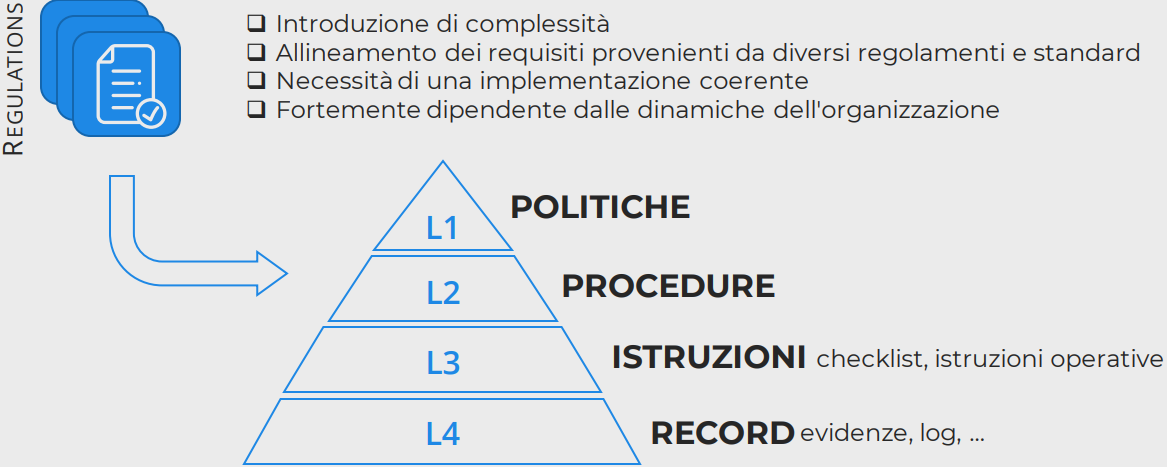
\includegraphics[keepaspectratio]{images/image18.png}}}

{}

{Esistono diverse caratteristiche che bisogna seguire per creare le
nuove normative, e sono:}

\begin{itemize}
\tightlist
\item
  {Proporzionalità}{~}{{[}+ IMPORTANTE{]}}{: la sicurezza non deve mai
  essere non sostenibile da una azienda;}
\item
  {Prevenzione}{: le norme devono prevenire gli incidenti e cercare di
  arrivare preparati in caso di attacco sapendo già le azioni da fare;}
\item
  {Condivisione}{: cioè riuscire a condividere con tutti le metodologie
  di attacchi e come proteggersi;}
\item
  {Uniformità}{: far sì che le normative siano applicabili fra loro e
  che tutte siano consone fra loro.}
\end{itemize}

{}

\subsection{\texorpdfstring{{GDPR}}{GDPR}}\label{h.yhkvkrud8nop}

{Regolamentazione europea nata per tutelare gli utenti finali e i loro
dati, tutte le aziende che operano in territorio europeo (anche con sede
all'estero) devono sottostare al GDPR.}

{}

{Il }{GDPR}{~si applica ai dati personali di cittadini europei che
vengono trattati in maniera interamente o parzialmente automatizzata.}

{I dati coinvolti sono:}

{\pandocbounded{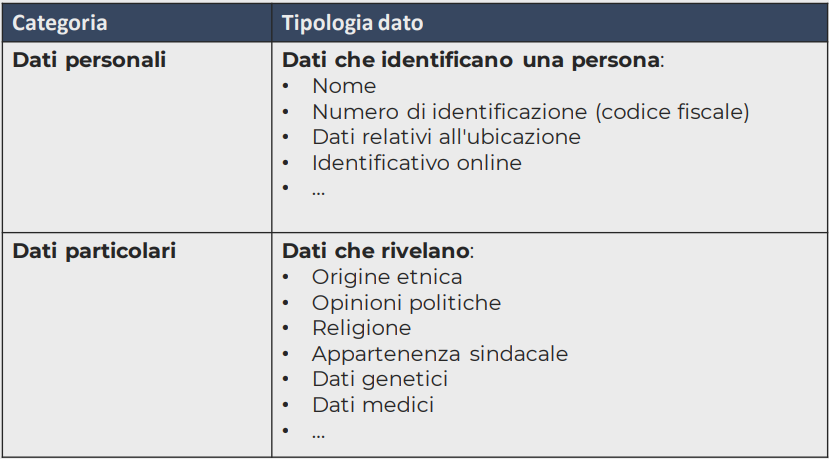
\includegraphics[keepaspectratio]{images/image36.png}}}

{}

{Nel GDPR si evidenziano anche alcuni attori:}

{\pandocbounded{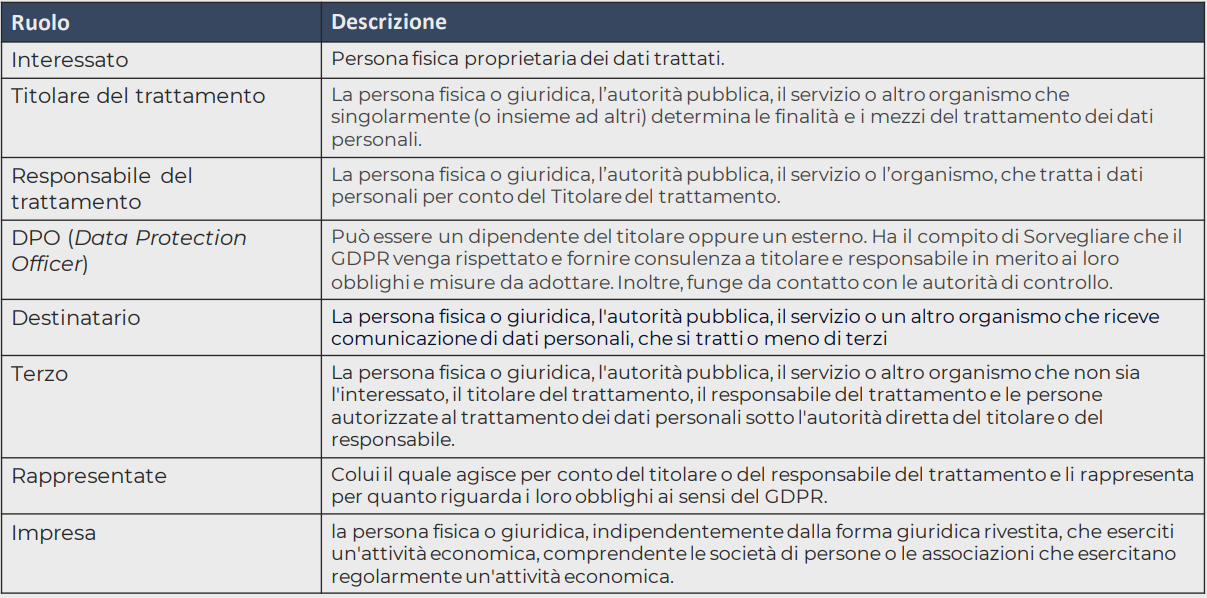
\includegraphics[keepaspectratio]{images/image110.png}}}

{}

{I diritti dell'interessato:}

{\pandocbounded{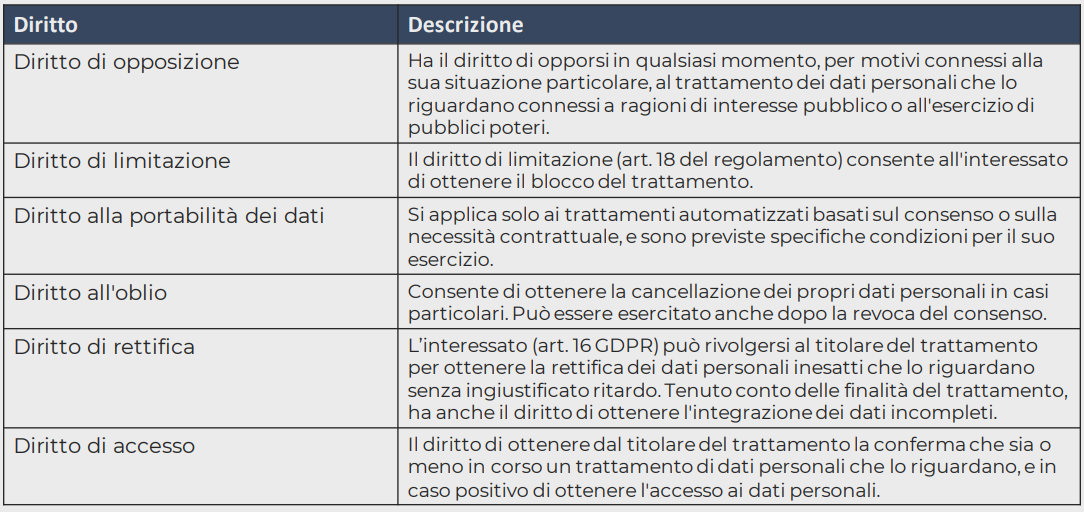
\includegraphics[keepaspectratio]{images/image69.png}}}

{Il diritto di portabilità dice che per esempio una banca quando
chiudete il conto per farlo in un'altra è obbligata a fare il passaggio
dei dati per voi.}

{}

{Il GDPR non impone normative tecniche precise ma è abbastanza generico
e astratto, ma impone misure di sicurezza per non cadere in sanzioni:}

{\pandocbounded{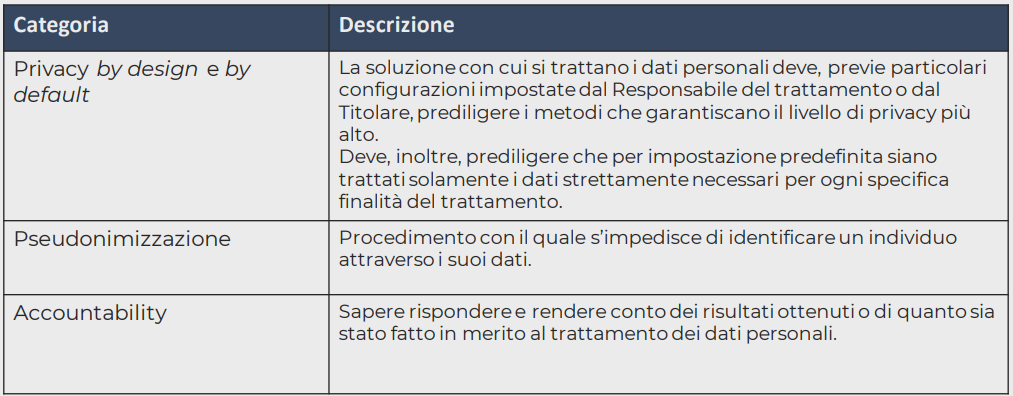
\includegraphics[keepaspectratio]{images/image47.png}}}

{alcune soluzioni reali invece per proteggere i dati sono:}

\begin{itemize}
\tightlist
\item
  {Anonimizzazione}{;}
\item
  {Separazione}{;}
\item
  {Conservazione cifrata e separata;}
\item
  {Cancellazione sicura e che avviene appena non più necessari}{;}
\item
  {Cifratura sia a riposo che quando trasmetti}{;}
\item
  {Applicare il principio del need-to-know}{;}
\item
  {Definire strategie di risposta agli incidenti e di prevenzione e
  gestione del rischio a livello aziendale}{;}
\item
  {~}{Richiedere e mantenere il minimo dei dati strettamente
  necessari}{.}
\end{itemize}

{}

{In caso non si rispettino le soluzioni riportate sopra si può intaccare
in un data breach, un data breach consiste in un evento per il quale si
può compromettere la riservatezza, l\textquotesingle integrità e la
disponibilità dei dati a perimetro. }

{Questa casistica può avvenire tramite alcuni di questi attacchi:}

\begin{itemize}
\tightlist
\item
  {comunicazione via email}{;}
\item
  {comunicazione fisica/di persona}{;}
\item
  {attacchi informatici fisici}{.}
\end{itemize}

{}

{In caso di attacchi il Titolare e/o il Responsabile sono tenuti a
notificarne l\textquotesingle avvenimento alle autorità entro 72 ore
tramite }{lesson learning}{~che riporta:}

\begin{itemize}
\tightlist
\item
  {la natura della violazione }
\item
  {nome e i dati di contatto del DPO }
\item
  {probabili conseguenze }
\item
  {misure adottate }
\end{itemize}

{ma va anche documentato ogni violazione ai dati personali e tenere
traccia delle comunicazioni tra le due figure.}

{}

{Il GDPR indica anche le varie responsabilità, infatti il testo dice:}

{}

{Chiunque subisca un danno materiale o immateriale causato da una
violazione del presente regolamento ha il diritto di ottenere un
risarcimento del danno dal }{titolare del trattamento}{~o dal
}{responsabile del trattamento}{.}

{}

{Il }{titolare }{coinvolto risponde per il danno cagionato dalle sua
azioni che violano il GDPR.}

{Se il }{responsabile }{non rispetta volutamente le indicazioni del
titolare sarà lui a rispondere al risarcimento.}

{}

{}

\subsection{\texorpdfstring{{PCI}}{PCI}}\label{h.mxf6ff3odjka}

{L'ente che ha redatto i vari standard è il PCI Council, opera a livello
globale a cui partecipano tutte le società che si occupano di
pagamenti.}

{}

{Va detto che in america è obbligatorio seguire le norme del PCI, in
europa no anche se fortemente consigliato visto che tutte le aziende che
non lo fanno probabilmente non riusciranno a stringere patti con altri
enti.}

{}

{Il suo scopo è guidare l'adozione di standard uniformi al livello di
sicurezza riguardo le informazioni e fornendo risorse per la messa in
sicurezza dell'ecosistema dei pagamenti.}

{I compiti principali sono:}

\begin{itemize}
\tightlist
\item
  {Definire standard di sicurezza per i pagamenti a livello globale }
\item
  {Validare e elencare prodotti e soluzioni che sono conformi con gli
  standard PCI (es. PCI SSC) e i relativi requisiti }
\item
  {Qualificare organizzazioni }
\item
  {Fornire un insieme di best practice per la sicurezza dei pagamenti}
\end{itemize}

{}

{Gli standard rilasciati dal PCI Council sono 7 e sono: }

{\pandocbounded{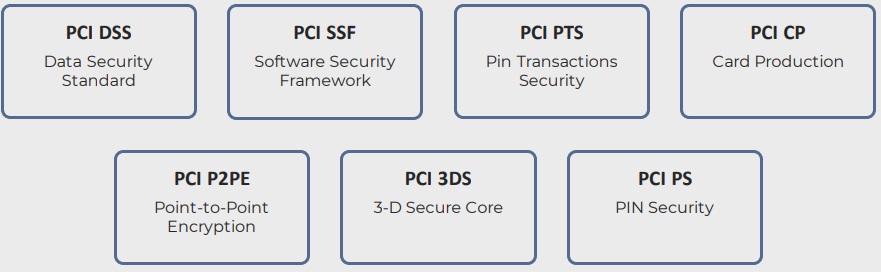
\includegraphics[keepaspectratio]{images/image24.png}}}

{}

{Sono presenti 8 principali ruoli definiti da PCI:}

{\pandocbounded{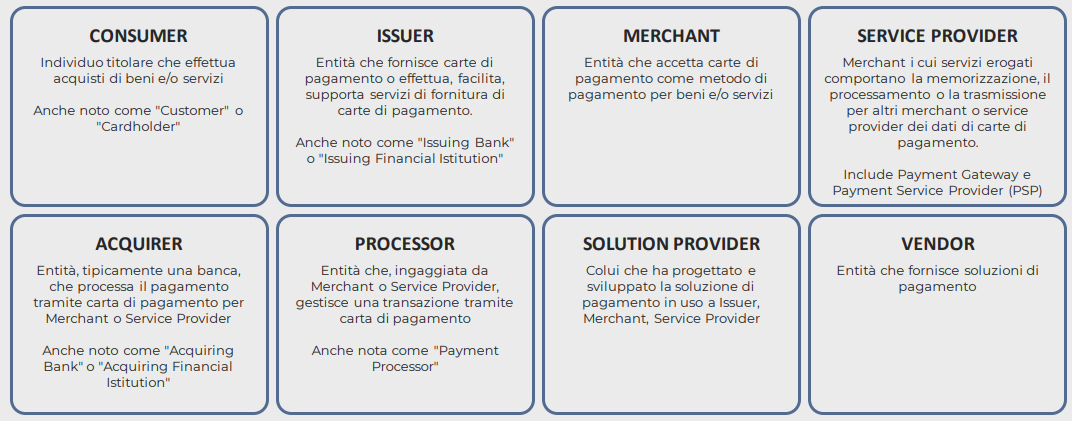
\includegraphics[keepaspectratio]{images/image38.png}}}

{}

{Ora possiamo vedere come i vari ruoli sono collocati nel processo di
pagamento:}

{\pandocbounded{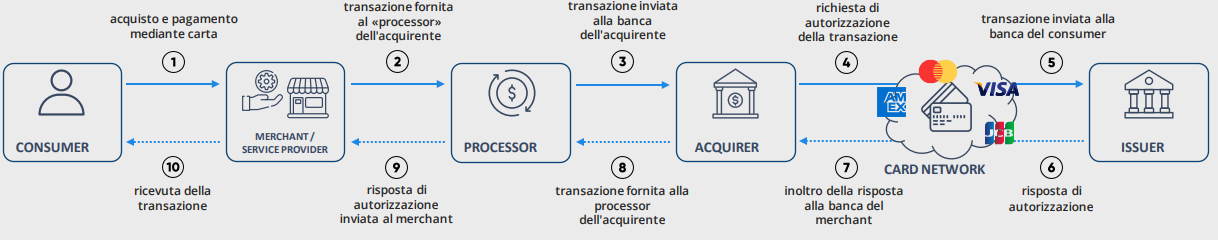
\includegraphics[keepaspectratio]{images/image121.png}}}

{il card network cambia in base alla carta.}

{}

{Per aderire al PCI è necessario attuare un processo continuo di
compliance e di sicurezza, strutturato secondo le seguenti fasi:}

{\pandocbounded{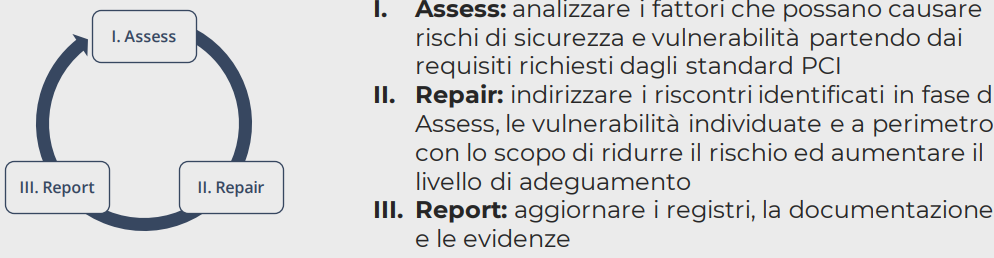
\includegraphics[keepaspectratio]{images/image39.png}}}

{I dati coinvolti dallo standard PCI sono detti account data, e sono
divisi fra cardholder data e sensitive authentication data:}

{\pandocbounded{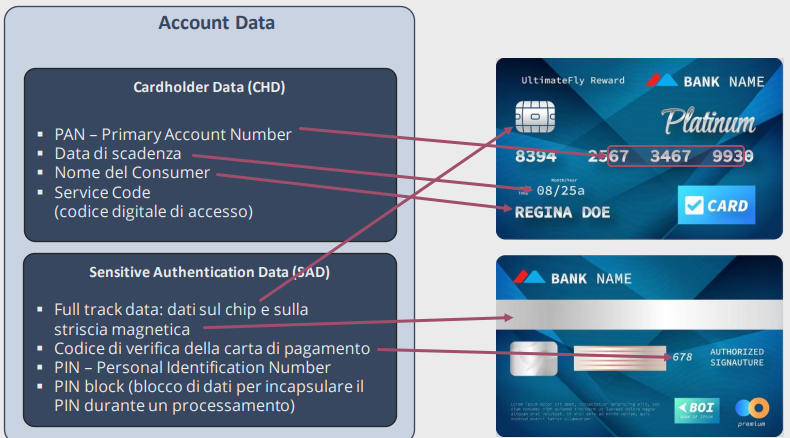
\includegraphics[keepaspectratio]{images/image113.png}}}

\subsubsection{\texorpdfstring{{PCI
SSF}}{PCI SSF}}\label{h.4bsj27at5uwt}

{Il PCI SSF (Secure Software Framework) è uno standard PCI che norma lo
sviluppo del software in maniera sicura. È composto da due parti, ognuna
delle quali si occupa di differenti aspetti applicativi: }

\begin{itemize}
\tightlist
\item
  {PCI Secure Software}
\item
  {PCI Secure Software Lifecycle}
\end{itemize}

{\pandocbounded{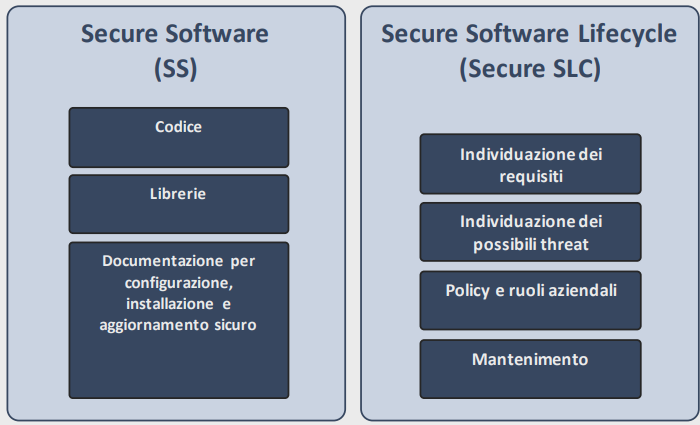
\includegraphics[keepaspectratio]{images/image115.png}}}

{}

{Seguendo il PCI SFF ti permettere di creare un secure payment
software:}

{\pandocbounded{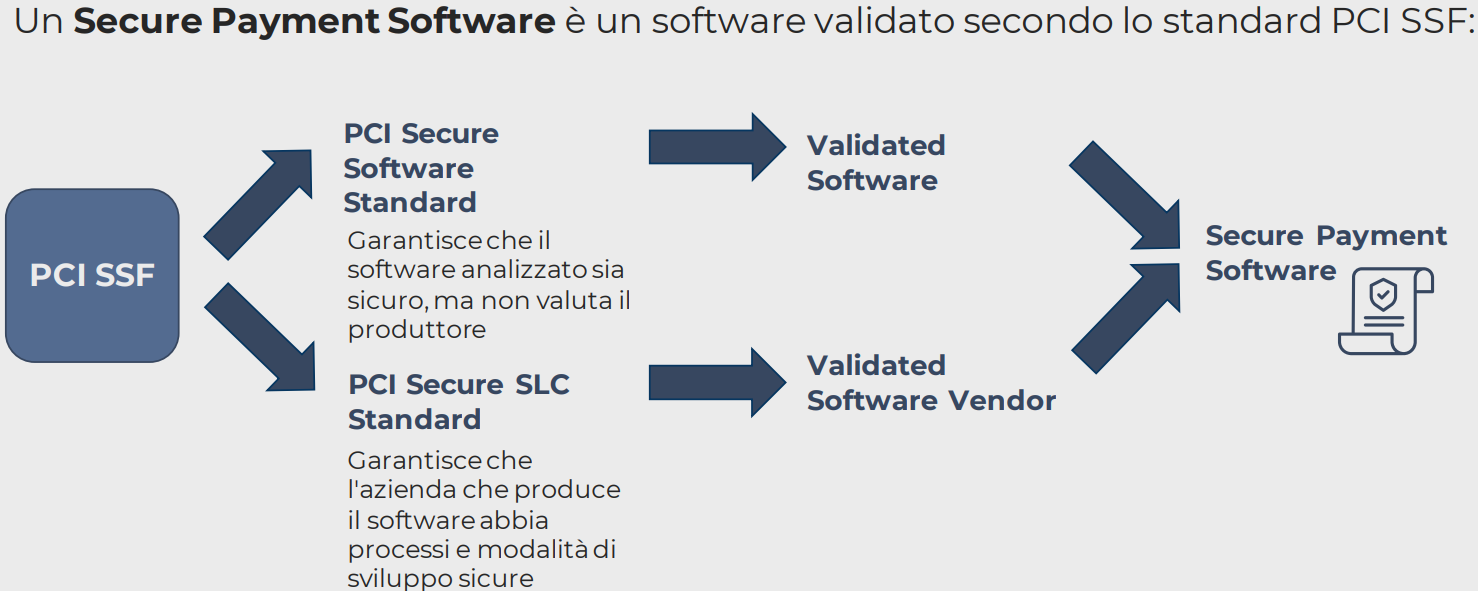
\includegraphics[keepaspectratio]{images/image59.png}}}

\subsubsection{\texorpdfstring{{PCI DSS}}{PCI DSS}}\label{h.kfjrowd3b53}

{\pandocbounded{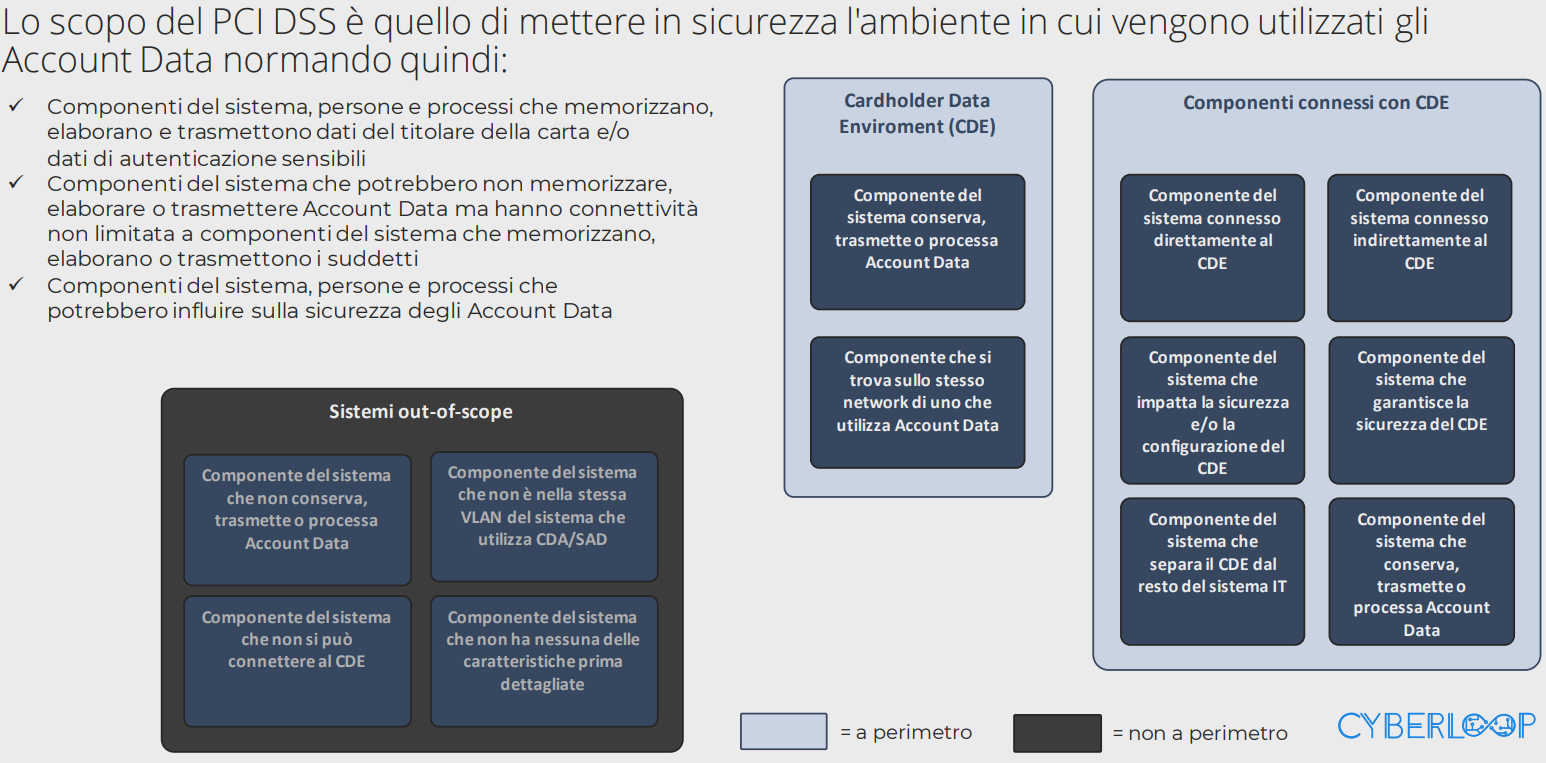
\includegraphics[keepaspectratio]{images/image68.png}}}

{Figure che il PCI DSS controlla:}

\begin{itemize}
\tightlist
\item
  {Coloro che lavorano sui dati}
\item
  {Coloro che non usano direttamente i dati ma ne hanno accesso}
\item
  {Coloro che potrebbero mettere a rischio i dati anche se fuori dal
  loro ambiente}
\end{itemize}

{}

{Lo standard PCI DSS migliora la sicurezza dei dati delle carte di
pagamento attraverso misure come la protezione dei dati dei titolari di
carta, il controllo degli accessi, il monitoraggio e il test delle reti,
e la gestione delle vulnerabilità. Queste misure aiutano le
organizzazioni a proteggere le informazioni sensibili da accessi non
autorizzati e frodi.}

\subsection{\texorpdfstring{{Standard
ISO}}{Standard ISO}}\label{h.sudhoj76kdg1}

{ISO è un\textquotesingle organizzazione internazionale indipendente che
sviluppa e pubblica standard tecnici per prodotti, servizi e sistemi a
livello globale, al fine di garantire la qualità,
l\textquotesingle efficienza e la sicurezza; contribuendo a creare un
ambiente di fiducia e cooperazione facilitando il commercio.}

{}

{\pandocbounded{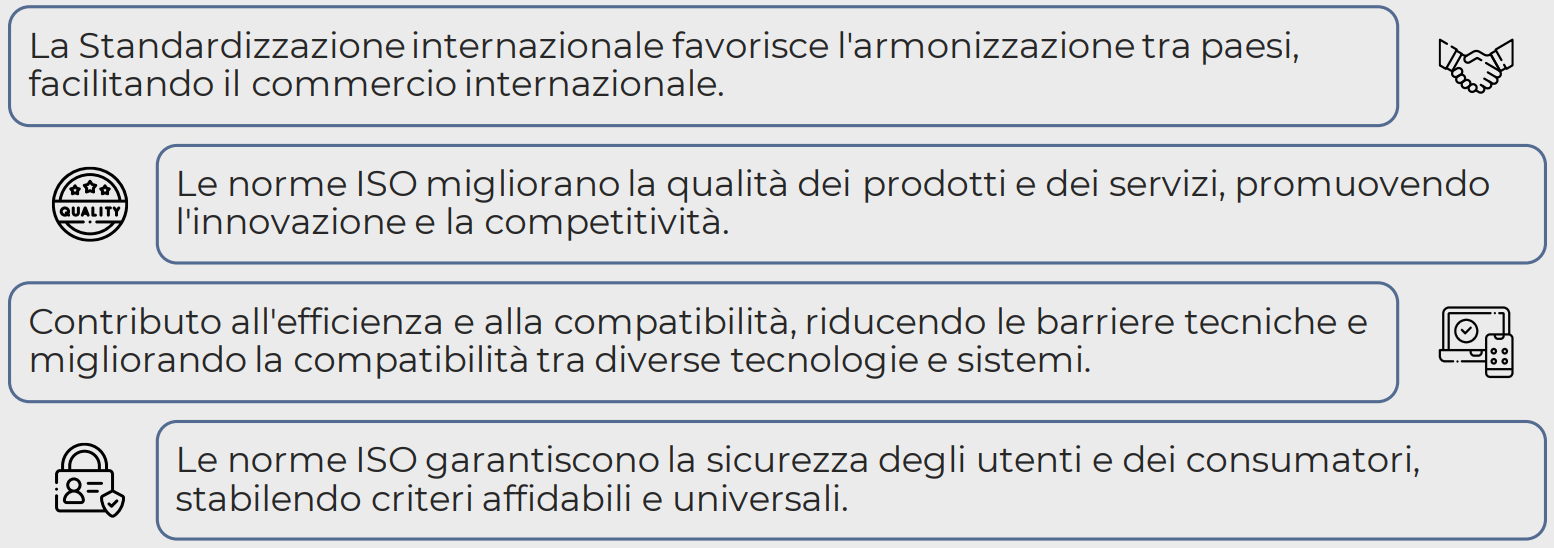
\includegraphics[keepaspectratio]{images/image21.png}}}

{}

{Una norma ISO è un documento tecnico che stabilisce: requisiti, linee
guida o specifiche per garantire la qualità,
l\textquotesingle affidabilità e la sicurezza di prodotti, servizi o
sistemi a livello internazionale. }

{Ogni norma è così strutturata: }{ISO 9001:2015 }{dove ogni elemento è:}

{\pandocbounded{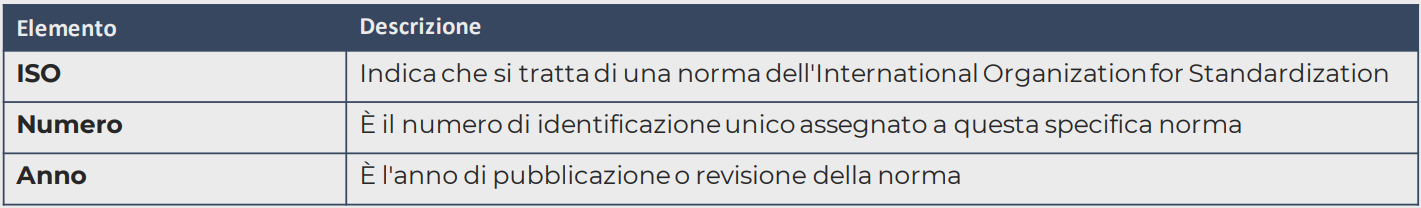
\includegraphics[keepaspectratio]{images/image33.png}}}

{}

{Le norme ISO sono cruciali nel commercio internazionale, poiché fungono
da linguaggio tecnico universale che supera barriere linguistiche e
culturali; agendo come un "passaporto commerciale" che semplifica gli
scambi internazionali. }

{}

{In sintesi, le norme ISO contribuiscono a creare un ambiente di fiducia
e cooperazione benefico per la comunità globale degli affari.}

{}

{Per garantire che le norma ISO vengano rispettate esistono due tipi di
audit:}

{\pandocbounded{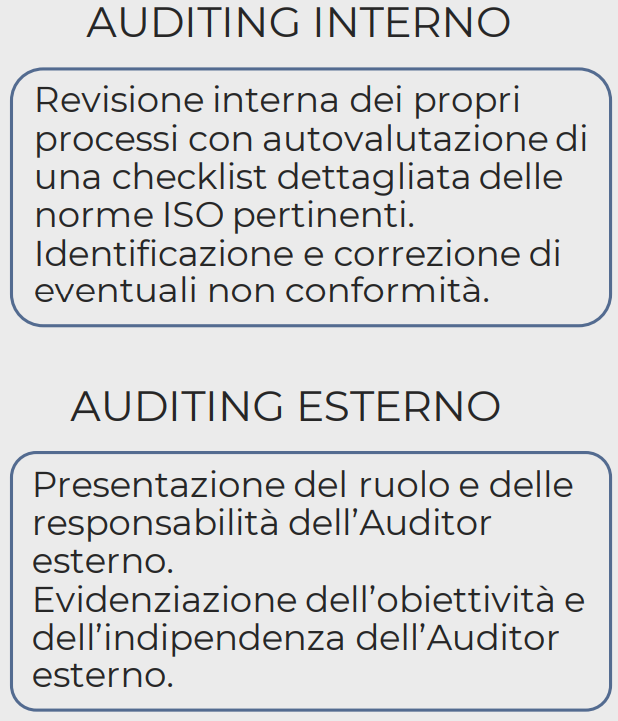
\includegraphics[keepaspectratio]{images/image16.png}}}

{Quello interno viene fatto in maniera autonoma per prepararsi a quello
esterno (come una simulazione d'esame) per poi passare a quello esterno
dove viene in azienda una figura incaricata dalla ISO. Se
}{l'auditor}{~alla fine del controllo pensa che tutto sia in regola
rilascia una certificazione.}

{Vediamo cos'è la certificazione:}

{\pandocbounded{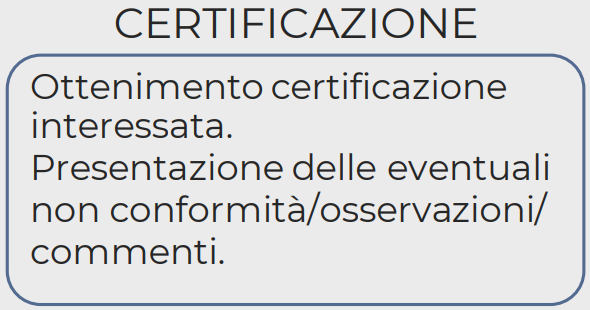
\includegraphics[keepaspectratio]{images/image99.png}}}

{}

{Ora vediamo alcune certificazioni ISO:}

{\pandocbounded{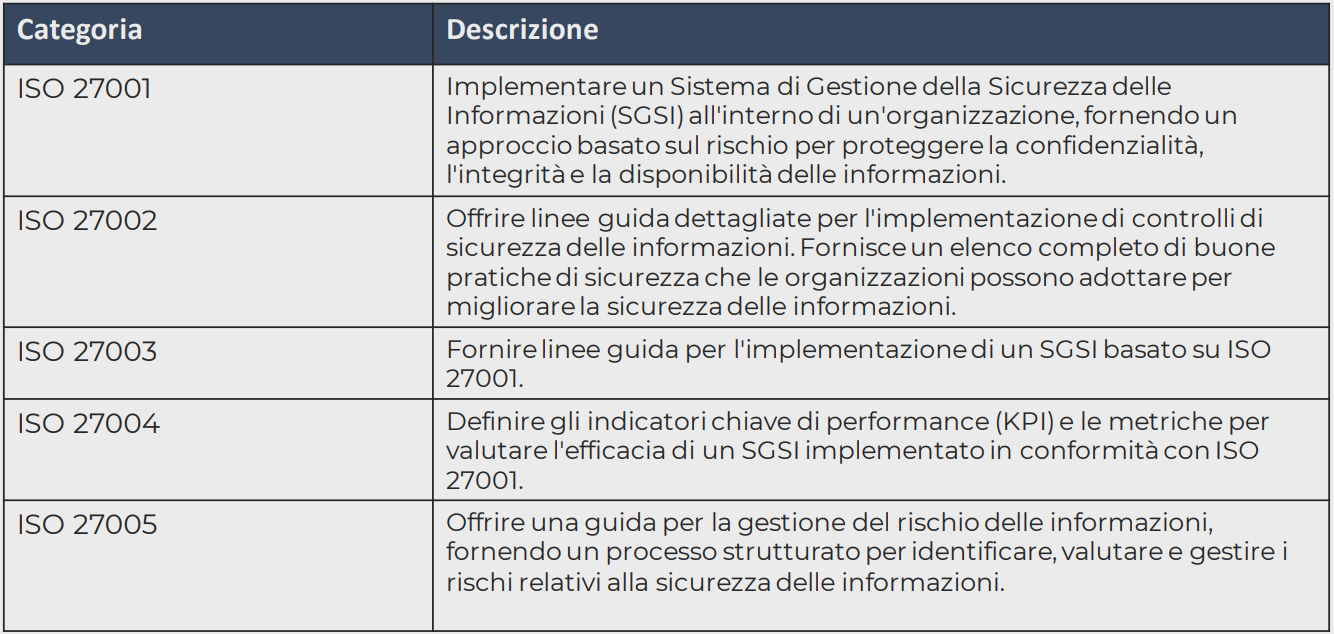
\includegraphics[keepaspectratio]{images/image93.png}}}

{Tutti questi standard fanno parte della famiglia degli ISO 27000 che
rappresenta un insieme di norme internazionali focalizzate sulla
sicurezza delle informazioni. Essa fornisce un quadro strategico e
operativo per sviluppare, implementare, monitorare e migliorare
continuamente i processi di gestione della sicurezza delle informazioni
all\textquotesingle interno di un\textquotesingle organizzazione.}

{}

{La famiglia ISO 27000 si concentra sul proteggere le informazioni da
minacce interne ed esterne, fornendo un approccio strutturato e basato
su best practice. }

{}

{Un'altra norma è la ISO 22301, dedicata al Business Continuity
Management (BCM), processo strategico che mira a identificare,
comprendere e mitigare i rischi che potrebbero minacciare la continuità
delle operazioni di un\textquotesingle organizzazione.}

{Per implementare la norma bisogna seguire principi fondamentali:}

{\pandocbounded{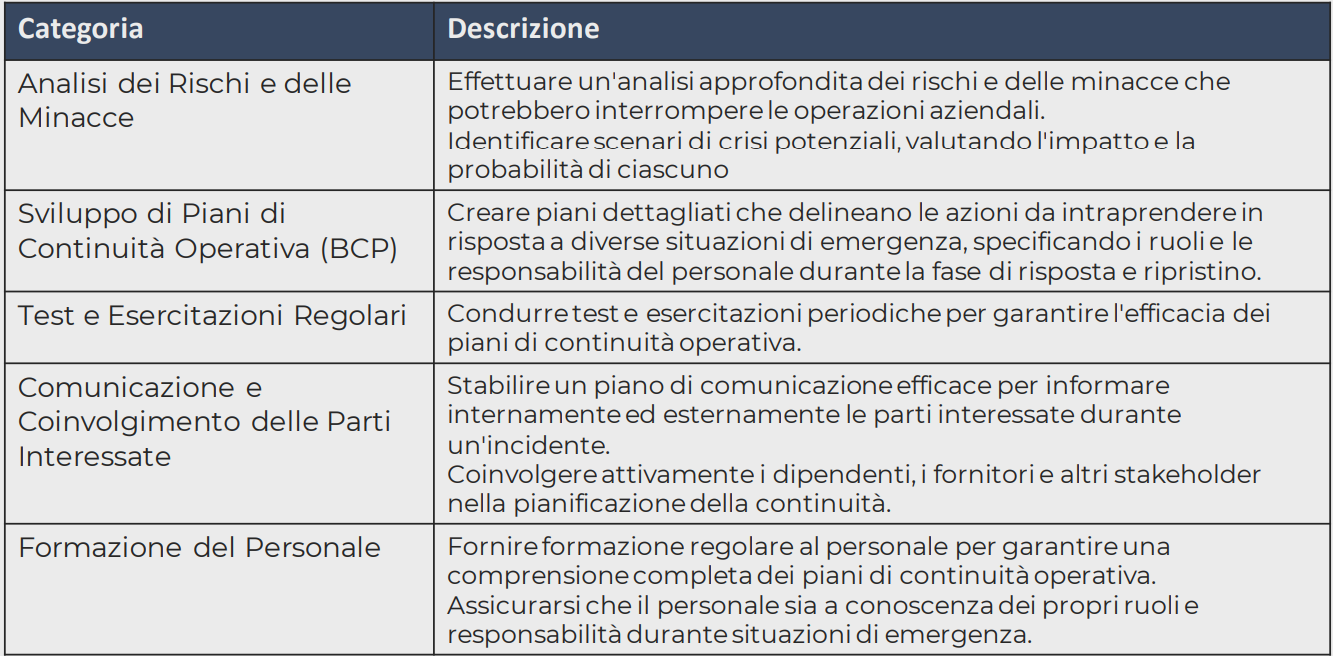
\includegraphics[keepaspectratio]{images/image54.png}}}

{Nel dettaglio la creazione di BCP è un processo essenziale per
garantire che un\textquotesingle organizzazione possa mantenere
operativi i suoi processi critici in situazioni di emergenza o crisi. }

\subsection{\texorpdfstring{{NIS2}}{NIS2}}\label{h.prv9opi5q8kc}

{Direttiva europea che aggiorna e amplia le misure di sicurezza per le
reti e i sistemi informativi degli operatori di servizi essenziali e dei
fornitori di servizi digitali, introducendo requisiti più rigorosi per
la gestione del rischio e la cooperazione tra gli Stati membri.}

{}

{Tra le principali novità proposte sono presenti:}

\begin{itemize}
\tightlist
\item
  {l\textquotesingle estensione del campo di applicazione a nuovi
  settori, come l\textquotesingle energia, i trasporti e la sanità }
\item
  {l\textquotesingle introduzione di obblighi aggiuntivi per gli
  operatori di servizi essenziali e i fornitori di servizi digitali.}
\end{itemize}

{}

{\pandocbounded{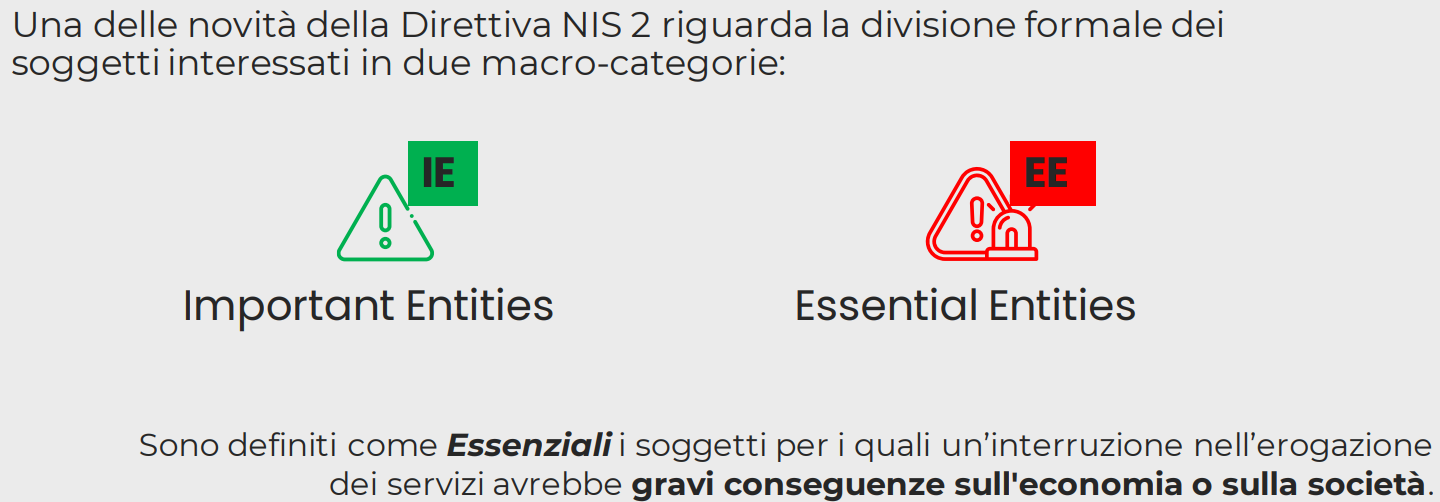
\includegraphics[keepaspectratio]{images/image104.png}}}{\pandocbounded{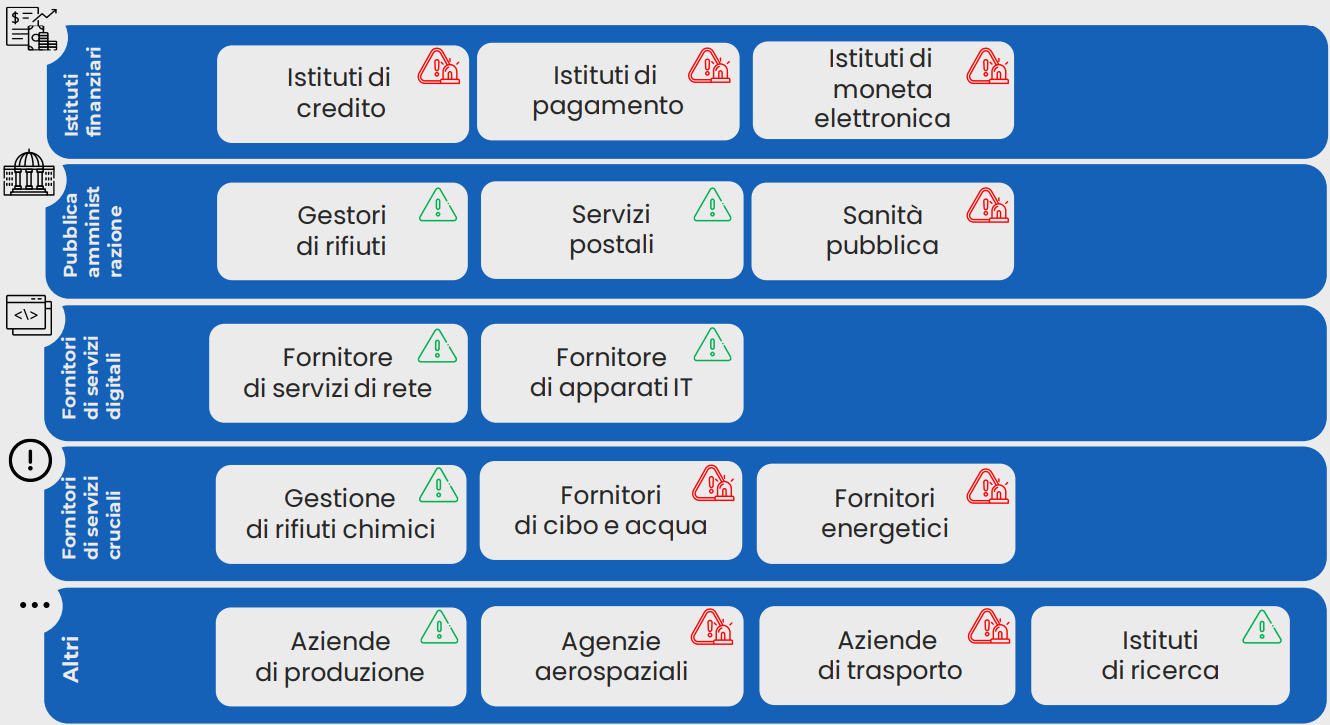
\includegraphics[keepaspectratio]{images/image60.png}}}

{}

{L'articolo 21 dice:}

{"Gli Stati membri provvedono affinché i soggetti essenziali e
importanti adottino misure tecniche, operative e organizzative adeguate
e proporzionate per gestire i rischi posti alla sicurezza dei sistemi
informatici e di rete che tali soggetti utilizzano nelle loro attività o
nella fornitura dei loro servizi, nonché per prevenire o ridurre al
minimo l\textquotesingle impatto degli incidenti per i destinatari dei
loro servizi e per altri servizi."}

{}

{Sostanzialmente tutti i soggetti indicati sopra devono prendere misure
per evitare rischi, queste misure sono definite e spiegate sempre
nell'articolo 21. Ecco alcuni esempi:}

\begin{itemize}
\tightlist
\item
  {Misura 3: continuità operativa, disaster recovery, ecc;}
\item
  {Misura 4: sicurezza della supply chain (catena di collaborazione fra
  aziende);}
\item
  {Misura 8: Crittografia e cifratura;}
\item
  {Misura 9: sicurezza risorse umane con controllo degli accessi e
  gestione utenti attivi (account di persone che non lavorano più li).}
\end{itemize}

{}

{}

{Un piano di adeguamento viene fatto per rendere conforme
un\textquotesingle azienda al NIS2, le fasi sono 4, nel dettaglio:}

\begin{enumerate}
\tightlist
\item
  {Analisi}{: Per far si che la sicurezza si adatti all'azienda si fanno
  delle }{interviste e valutazioni}{, è necessaria assoluta
  collaborazione fra tutti i soggetti per definire un piano di
  adeguamento efficace.}
\end{enumerate}

{}

\begin{enumerate}
\setcounter{enumi}{1}
\tightlist
\item
  {Definizione}{: }{Si definisce il piano completo tenendo in
  considerazione le criticità per il business individuate nelle fasi
  precedenti}{, prioritizzando, così, le attività (es: definizione dei
  ruoli, definizione di KPI di sicurezza cioè un indice per diverse
  casistiche come il numero di attacchi ricevuti).}
\end{enumerate}

{Il NIS2 impone che anche aziende partner abbiamo lo stesso livello di
sicurezza. }

{}

\begin{enumerate}
\setcounter{enumi}{2}
\tightlist
\item
  {Implementazione:}{~si va ad }{implementare tutto quello concordato
  precedentemente}{, per farlo dobbiamo capire quanto c'è di differenza
  tra dove siamo ora e dove vogliamo arrivare, questo spazio si dice gap
  e può essere:}
\end{enumerate}

\begin{itemize}
\tightlist
\item
  {Gap Tecnologico}{: comporta la necessità, comunemente, di aggiornare
  il sistema IT dal punto di vista sia infrastrutturale sia software.}
\item
  {Gap Formativo}{: è un grosso ostacolo per la corretta messa in atto
  del piano definito, pertanto è necessaria una formazione adeguata al
  ruolo che si ricopre.}
\end{itemize}

{}

\begin{enumerate}
\setcounter{enumi}{3}
\tightlist
\item
  {Monitoraggio}{: }{controllo che tutto sia rispettato}{, effettuare
  esami o simulazioni di attacco per vedere se i dipendenti sono
  preparati.}
\end{enumerate}

{}

{Per vedere gli impatti andare nelle slides:}

{~Laboratorio di sicurezza dei sistemi informatici e privacy - 01
Normative - V1R0.pdf }

{\href{https://www.google.com/url?q=https://liveunibo.sharepoint.com/:b:/s/LoPTSI_SedediImola/ET-eiun98a9BjHi7_UkTr2UBPhpsrulx9aFysJbld1LSZg?e\%3DEHG2ot&sa=D&source=editors&ust=1734628852089079&usg=AOvVaw0eUInyO2oXFn7RG-sdHFkp}{Slides}}

{da pagina 82 a 90}

\subsection{\texorpdfstring{{Regolamento
DORA}}{Regolamento DORA}}\label{h.2z3cfhhuhtjw}

{Il Digital Operation Resilience Act (DORA), pacchetto europeo per la
digitalizzazione del settore finanziario, }{mira a garantire adeguati
meccanismi di salvaguardia in caso di attacchi informatici}{~e a
consolidare i requisiti per la }{prevenzione del rischio ICT nel settore
finanziario}

{}

{Pone particolare attenzione a cinque aree di sicurezza:}

\begin{itemize}
\tightlist
\item
  {Gestione del rischio ICT }
\item
  {Gestione del rischio ICT nei rapporti con terze parti }
\item
  {Governo della}{~condivisione di informazioni tra entità finanziarie }
\item
  {Formulazione di reportistica legata a importanti incidenti ICT}
\item
  {Modalità di test per la verifica della resilienza digitale}
\end{itemize}

{}

{\pandocbounded{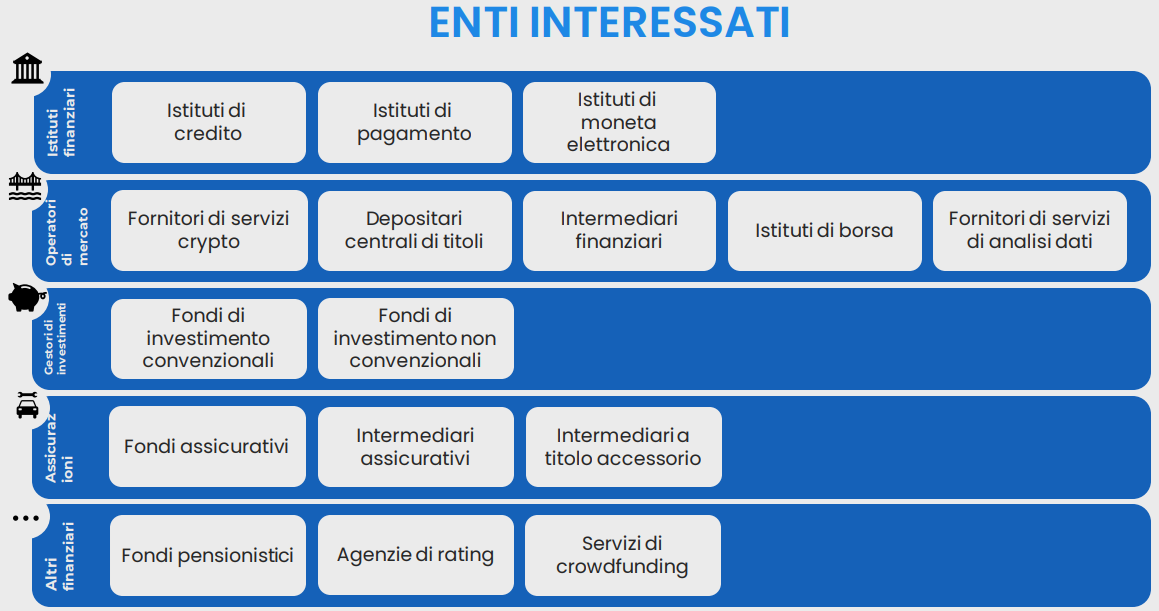
\includegraphics[keepaspectratio]{images/image53.png}}}

{}

{Il DORA è nato proprio per creare una regolamentazione a parte per
questo genere di enti per via della complessità di gestione e di
protezione.}

{}

{Questa normativa non sostituisce altre normative preesistenti come NIS2
ma le integra, infatti il DORA è maggiormente orientato alla assicurarsi
la presenza di strategie, framework (modalità di lavoro che facilità) e
processi di governo.}

{}

{}

{}

{\pandocbounded{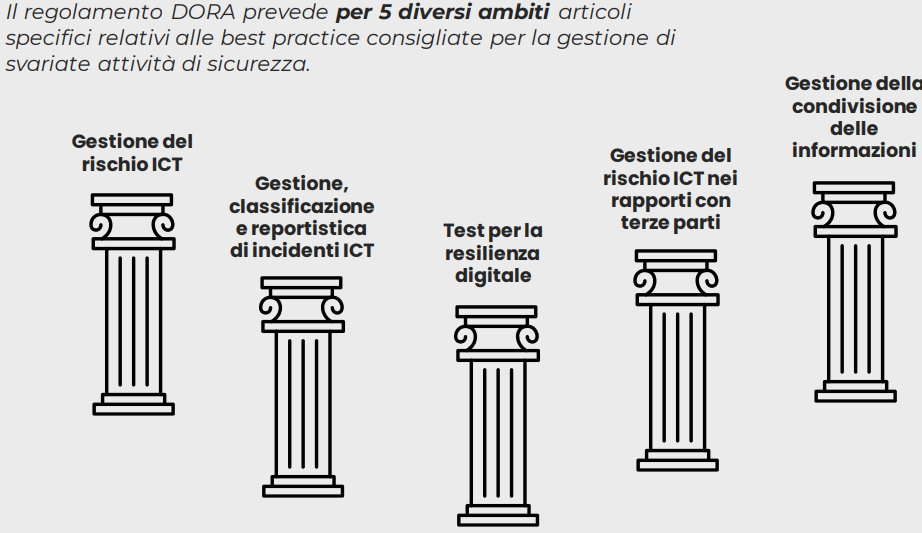
\includegraphics[keepaspectratio]{images/image80.png}}}{\pandocbounded{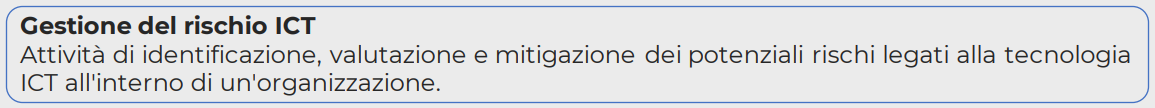
\includegraphics[keepaspectratio]{images/image101.png}}}{\pandocbounded{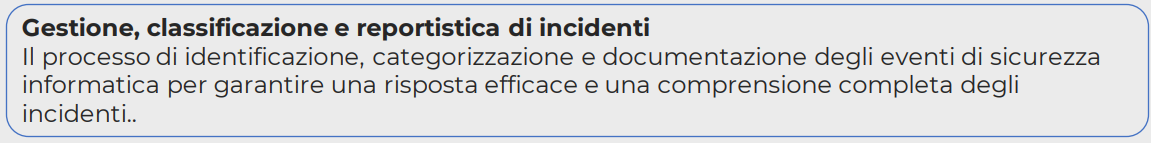
\includegraphics[keepaspectratio]{images/image45.png}}}{\pandocbounded{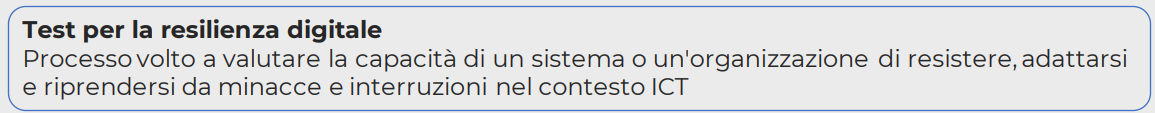
\includegraphics[keepaspectratio]{images/image76.png}}}{\pandocbounded{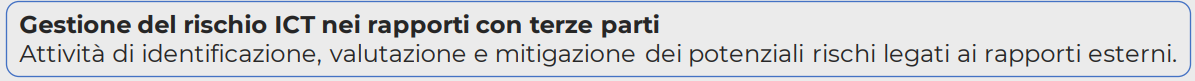
\includegraphics[keepaspectratio]{images/image41.png}}}{\pandocbounded{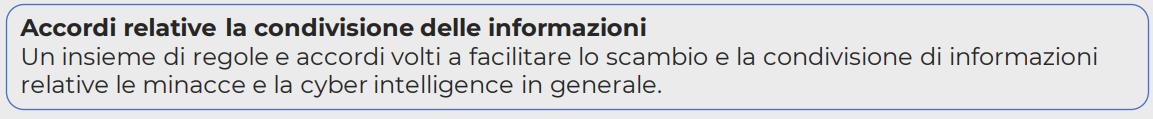
\includegraphics[keepaspectratio]{images/image88.png}}}

{}

{\pandocbounded{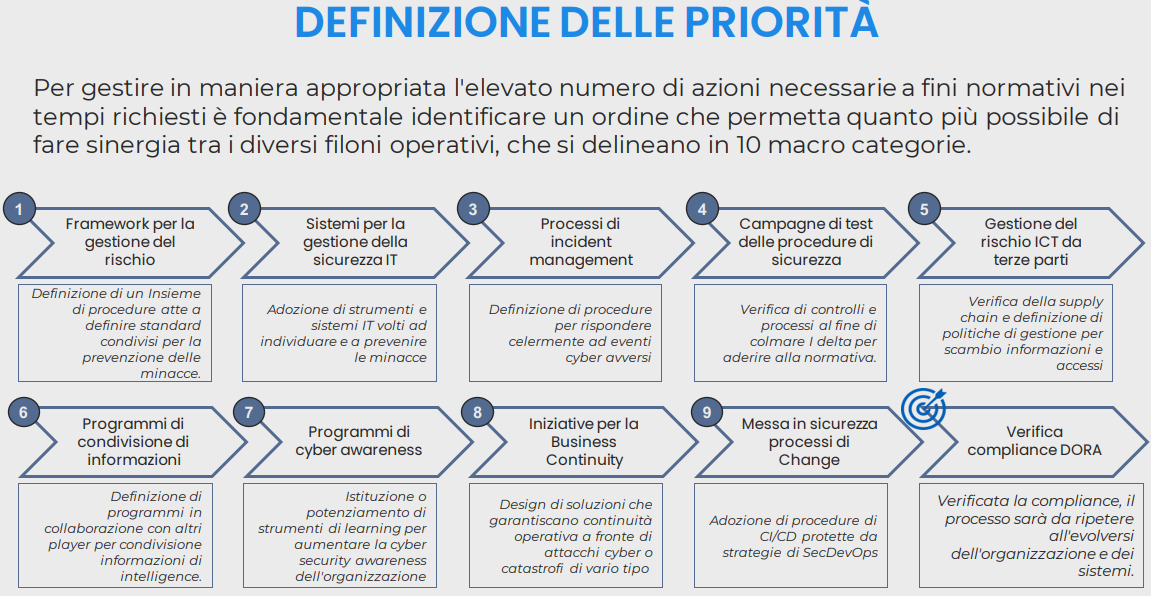
\includegraphics[keepaspectratio]{images/image73.png}}}

{}

{}

\section{\texorpdfstring{{Active directory
security}}{Active directory security}}\label{h.c1qub11isjm}

{Active Directory è un sistema server centralizzato, fondato sui
concetti di dominio e di directory, ovvero un insieme di servizi di
rete, meglio noti come directory service, gestiti da un domain
controller. Tale sistema, inoltre, definisce la modalità con cui vengono
assegnate agli utenti tutte le risorse di rete attraverso i concetti di:
account utente, account computer, cartelle condivise,.. secondo
l\textquotesingle assegnazione da parte
dell\textquotesingle amministratore di sistema di Group Policy.}

{}

{Active Directory Service è un\textquotesingle infrastruttura
informativa condivisa per gestire elementi e risorse di rete in ambiente
Windows, tra le principali caratteristiche vi sono le seguenti: }

\begin{itemize}
\tightlist
\item
  {Erogazione di un archivio centrale per l\textquotesingle identità e
  le informazioni sull\textquotesingle account }
\item
  {Assegnazione di un identificatore univoco a ciascuno degli oggetti}
\item
  {Mappatura dei nomi delle risorse di rete ai loro rispettivi indirizzi
  di rete}
\item
  {~Inclusione dei disposizioni di controllo
  dell\textquotesingle accesso, limitando la disponibilità delle
  informazioni della directory agli utenti autorizzati}
\end{itemize}

\subsection{\texorpdfstring{{Architettura}}{Architettura}}\label{h.5fn5o7cyexdf}

{Fisicamente, il sistema Active Directory è costituito da uno o più
Windows Server che eseguono un servizio chiamato Controller di dominio.
}

{Un Directory Service è un servizio che archivia e organizza gli oggetti
in un archivio dati centralizzato e gerarchico: }

\begin{itemize}
\tightlist
\item
  {un oggetto directory è un oggetto che contiene uno o più attributi }
\item
  {gli oggetti sono identificati da un nome univoco, possono essere
  creati, aggiornati ed eliminati nella directory }
\item
  {I client possono recuperare il contenuto degli oggetti directory
  leggendo gli attributi di un oggetto specifico o eseguendo query per
  qualsiasi oggetto che corrisponda ai criteri specificati dal client}
\end{itemize}

\subsection{\texorpdfstring{{Directory
tree}}{Directory tree}}\label{h.2cvn0rcw1jb4}

{Un concetto centrale nel servizio è la directory tree che possiede le
seguenti caratteristiche: }

\begin{enumerate}
\tightlist
\item
  {Ogni oggetto ha un solo padre (tranne la radice
  dell\textquotesingle albero, il domain controller); }
\item
  {Ogni oggetto può avere zero o più oggetti }{figlio}{, dove a ciascuno
  viene assegnato un nome (RDN) univoco tra i fratelli; }
\item
  {Ogni oggetto della directory può essere identificato in modo univoco
  da tutti gli oggetti del servizio di directory dal suo nome distinto
  (DN), che si forma }{concatenandolo
  con}{~}{l\textquotesingle RDN}{~dell\textquotesingle oggetto. }
\end{enumerate}

\subsection{\texorpdfstring{{Dominio}}{Dominio}}\label{h.uzsslk8dfc2q}

{Un dominio è un insieme di utenti e computer che condividono una
namespace e un\textquotesingle infrastruttura di gestione comune. Tra le
caratteristiche della strutture vi è:}

\begin{itemize}
\tightlist
\item
  {la presenza di almeno un computer membro dell\textquotesingle insieme
  che funge da Domain Controller (DC) che ospita un elenco per
  identificare tutti i membri del dominio }
\item
  {la fruizione da parte del dominio di diversi servizi ai suoi
  }{client,}{~principalmente relativi alla sicurezza e alla gestione }
\item
  {l' attuazione da parte del DC dell' autenticazione dei membri,
  creando un\textquotesingle unità di fiducia per i suoi membri }
\item
  {la condivisione del proprio identificativo tra tutti i membri }
\end{itemize}

\subsection{\texorpdfstring{{Sicurezza}}{Sicurezza}}\label{h.c5edo6xmc1ab}

{Esistono due oggetti fondamentali:}

\begin{itemize}
\tightlist
\item
  {Security Principal: è in identità associata ad un utente umano o ad
  un programma che può essere autenticato, tale identità deve possedere
  minimo due attributi: un nome e un id che lo identificano in modo
  univoco rendendolo significativo per il sistema.}
\item
  {Security Identifier (SID): È l'id per poter identificare il security
  principal ed è quello che viene controllato per accedere agli oggetti.
  Spesso il SID corrisponde ad un utente umano ma può anche essere un pc
  o un servizio}
\end{itemize}

\subsubsection{\texorpdfstring{{Autenticazione/Autorizzazione}}{Autenticazione/Autorizzazione}}\label{h.9hwc1lanagzu}

{Tutta l'infrastruttura permette agli utenti di effettuare l'accesso
alle informazioni richieste mediante un' autenticazione e un'
autorizzazione:}

\begin{itemize}
\tightlist
\item
  {~I security principals del dominio sono tutti disponibili nel domain
  controller }
\item
  {Il dominio funge da fonte primaria di identità per i clienti del
  dominio }
\item
  {Il dominio, attraverso i protocolli di sicurezza pertinenti, fornisce
  la base per l\textquotesingle autenticazione
  all\textquotesingle interno di esso }
\item
  {Durante il processo di autenticazione, il dominio fornisce
  informazioni di autorizzazione sotto forma di identità aggiuntive che
  rappresentano gruppi, consentendo di prendere decisioni di
  autorizzazione.}
\end{itemize}

\subsubsection{\texorpdfstring{{LDAP}}{LDAP}}\label{h.9yklstq49j64}

{LDAP (Lightweight Directory Access Protocol) è un protocollo
multipiattaforma utilizzato per : }

\begin{itemize}
\tightlist
\item
  {autenticazione ai servizi di directory }
\item
  {comunicazione tra l\textquotesingle applicazione e i server dei
  servizi di directory che memorizzano e condividono informazioni su
  utenti, password e account di computer.}
\end{itemize}

{~A causa dell\textquotesingle architettura di Active Directory, una
volta violato un computer collegato a un dominio,
l\textquotesingle attaccante può essere in grado di mappare la rete,
individuare gli account e le risorse sensibili e stimare le
vulnerabilità. Tale processo è reso possibile attraverso
l'interrogazione del DC utilizzando il protocollo LDAP.}

{}

{Il protocollo consente diversi tipi di autenticazione (RFC 2829), per
esempio:}

\begin{itemize}
\tightlist
\item
  {Autenticazione anonima usata per disabilitare o aggiungere
  restrizioni di controllo degli accessi }
\item
  {Autenticazione nome/password (non sicura e non adatta se si vuole
  diritto di riservatezza) }
\item
  {Autenticazione mediante un digest (non espone la password in chiaro
  ma la password deve essere salvata in chiaro e precalcolato il digest
  lato server) ~}
\item
  {Autenticazione client basata su certificati}
\end{itemize}

\subsection{\texorpdfstring{{Connessioni tra
domini}}{Connessioni tra domini}}\label{h.j5z4w5uqkw1l}

{Ne esistono di diversi tipi:}

\begin{itemize}
\tightlist
\item
  {Unidirezionali}{: solo un dominio dei due della connessione, A e B,
  può accedere all'altro dominio; A accede a B ma non il contrario.}
\end{itemize}

{}

\begin{itemize}
\tightlist
\item
  {Bidirezionale}{: Il dominio A si fida del dominio B e il dominio B si
  fida del dominio A. Questa configurazione significa che le richieste
  di autenticazione possono essere tra i due domini in entrambe le
  direzioni. Alcune relazioni bidirezionali possono essere di due tipi
  (transitive }{o intransitive)}{~a seconda del tipo di fiducia che si
  sta creando }
\end{itemize}

{}

\begin{itemize}
\tightlist
\item
  {Transitivo}{: può essere utilizzato per estendere le relazioni di
  fiducia con altri domini; se B si fida di C allora anche A può
  accedere a C perché si fida di B }
\end{itemize}

{}

\begin{itemize}
\tightlist
\item
  {Intransitiva}{: può essere utilizzata per negare le relazioni di
  fiducia con altri domini}
\end{itemize}

\subsection{\texorpdfstring{{Strumenti di
sicurezza}}{Strumenti di sicurezza}}\label{h.luhz00iqftqx}

\subsubsection{\texorpdfstring{{GPO}}{GPO}}\label{h.6nl9uwg4kdp0}

{Un Group Policy Object (GPO) è un gruppo di impostazioni create
utilizzando la Microsoft Management Console (MMC). Le GPO possono essere
associate a uno o più contenitori di Active Directory, compresi siti,
domini o unità organizzative (UO). I Group Policy Object , se utilizzati
correttamente, consentono di aumentare la sicurezza dei computer degli
utenti, di difendersi dalle minacce interne e dagli attacchi esterni e,
in parte, di controllare ciò che gli utenti possono o non possono fare
su un sistema informatico.}

{}

\subsubsection{\texorpdfstring{{ACL}}{ACL}}\label{h.a7hs27gvjnk8}

{Access Control Lists (ACLs) sono le impostazioni che definiscono le
autorizzazioni in Active Directory. }

{Ciascuna di esse deve definire: }

\begin{itemize}
\tightlist
\item
  {chi può accedere }
\item
  {a quale oggetto si può accedere }
\item
  {il tipo di accesso (ACE) Ogni ACE si riferisce al security principal
  (Utenti, Gruppi e Processi) e definisce i diritti di accesso
  all\textquotesingle oggetto (consentito o negato) per quel security
  principal. Inoltre le ACL sono molto flessibili e possono essere
  aggiunte altre ACE in base alle necessità.}
\end{itemize}

{\pandocbounded{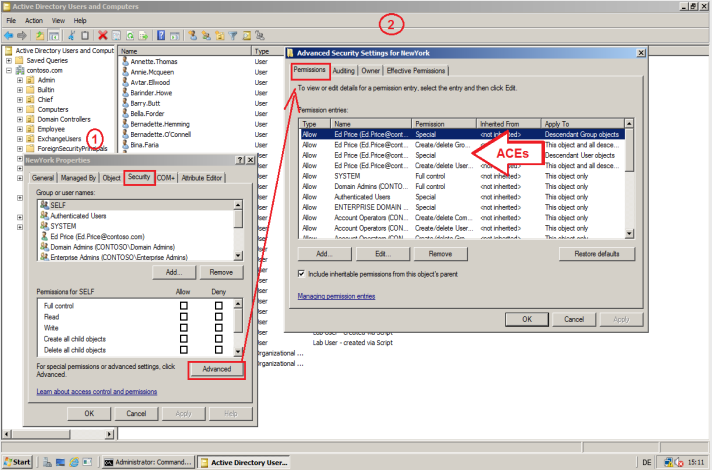
\includegraphics[keepaspectratio]{images/image108.png}}}

{}

{Un tipico ACE contiene le seguenti informazioni: }

\begin{enumerate}
\tightlist
\item
  {Un identificatore di sicurezza (SID), unico in tutto il dominio }
\item
  {Una maschera di accesso(32 bit) che definisce le operazioni
  consentite o negate }
\item
  {Un flag che indica il tipo di ACE ( per consentire, per negare o di
  controllo di sistema) }
\item
  {Un insieme di flag che determinano se i contenitori o gli oggetti
  figli possono ereditare l'ACE del loro genitore }
\end{enumerate}

\paragraph{\texorpdfstring{{Come
funziona}}{Come funziona}}\label{h.k8i73ag2mgjo}

{Quando un mandante di sicurezza invia una Richiesta di accesso per un
oggetto, il SID della richiesta viene confrontato con
l\textquotesingle Elenco di controllo degli accessi. }

{Se il SID corrisponde al SID presente nell\textquotesingle ACL, al
mandante di sicurezza viene concesso l\textquotesingle accesso
all\textquotesingle oggetto in base ai diritti predefiniti (es. lettura,
scrittura, modifica, cancellazione, ecc.). }

{Esistono comunemente due tipi di ACL:}

\begin{enumerate}
\tightlist
\item
  {~Discretionary access control list }{(DACL)}{~che definisce i
  principi di sicurezza che vengono concessi o negati. }
\item
  {System access control list (SACL) che garantisce agli admin il
  privilegio di registrare i log e i tentativi di accesso agli oggetti
  protetti}
\end{enumerate}

\subsection{\texorpdfstring{{Aggiungere un
PC}}{Aggiungere un PC}}\label{h.esbzs95cto1y}

{Quando un pc è aggiunto a dominio cosa succede?}

\begin{enumerate}
\tightlist
\item
  {~Gli account utente del dominio diventano utenti validi del sistema e
  possono accedervi (a meno che non si applicano restrizioni). }
\item
  {Gli amministratori del dominio acquisiscono diritti amministrativi
  sul sistema. }
\item
  {Il computer stesso ottiene un account nel dominio e lo utilizza per
  autenticarsi. }
\item
  {Il nome del computer viene registrato nel DNS del dominio. }
\item
  {Le Group Policy definite nel dominio e indirizzate ai computer
  influiscono sul sistema. }
\item
  {Le Group Policy definite nel dominio e destinate agli utenti
  influiscono su qualsiasi utente del dominio che accede al computer. }
\end{enumerate}

\subsection{\texorpdfstring{{NTLM}}{NTLM}}\label{h.jhpn0g28git9}

{Microsoft all' interno della propria architettura, dal 2008, ha creato
un protocollo di autenticazione, denominato NT LAN Manager (NTLM), che
consente l'autenticazione reciproca di computer e server diversi.}

{}

{Il protocollo prevede l'autenticazione di un client mediante un nome
utente e una password associata attraverso uno scambio di informazioni
tra il dispositivo dell'utente e un server, il quale conosce i dati di
login e quindi può controllare l'accesso e autorizzarlo. }

{\pandocbounded{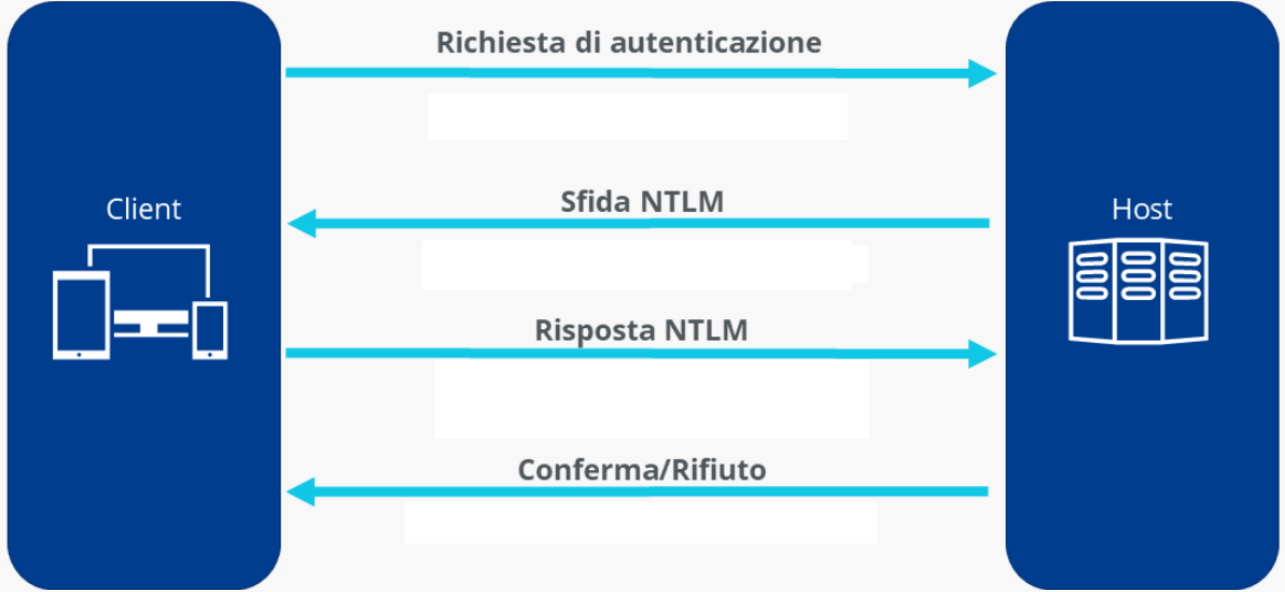
\includegraphics[keepaspectratio]{images/image102.png}}}

\subsubsection{\texorpdfstring{{Vantaggi}}{Vantaggi}}\label{h.cqzcwpdg5pjn}

{Un vantaggio di NTLM è che per l'autenticazione non bisogna inviare
sulla rete password non protette. La trasmissione dal client al server
avviene unicamente sotto forma di valore hash. Questo garantisce
certamente un maggiore livello di sicurezza.}

\subsubsection{\texorpdfstring{{Svantaggi}}{Svantaggi}}\label{h.uysbcrecuf65}

{Se il valore hash dovesse venir intercettato, può venir meno la
sicurezza promessa dal sistema. Infatti la password è crittografata
tramite MD4, un metodo crittografico considerato ormai poco sicuro in
quanto con i pc esistenti oggi tali valori hash possono essere
}{decodificati}{~abbastanza facilmente attraverso un attacco brute
force}

\subsection{\texorpdfstring{{KERBEROS}}{KERBEROS}}\label{h.9kd4k9ac59hc}

{Kerberos, è un servizio di autenticazione che, consente autenticarsi
attraverso una rete insicura in maniera sicura, si assegna una chiave
unica a ciascun utente che si collega alla rete e incorporando poi
queste chiavi nei messaggi inviati dagli utenti (chiave simmetrica) e
per la verifica delle identità, si utilizzano delle codifiche
crittografate e una terza entità, responsabile della validazione
dell'autenticazione. }

{}

{Il servizio è un progetto open source del Kerberos Consortium ed è la
tecnologia di autorizzazione standard di Microsoft Windows introdotta
già nelle prime apparecchiature di Windows 2000 in sostituzione di NTLM.
Kerberos gestisce l'autenticazione Single }{Sing}{~On gestendo le
credenziali in tutta la foresta ogni volta che si cerca di accedere alle
risorse, dopo l'accesso iniziale al dominio tramite Winlogon.}

\subsubsection{\texorpdfstring{{Funzionamento}}{Funzionamento}}\label{h.bvnu1qjltmau}

\paragraph{\texorpdfstring{{Step 1}}{Step 1}}\label{h.p927xx2qfydu}

{Client invia una richiesta (krb\_as\_req) all'AS chiedendo un Ticket
per accedere all'App Server. Tale richiesta è strutturata in questo
modo: }

\begin{itemize}
\tightlist
\item
  {Timestamp (cifrato con user psw) }
\item
  {Username }
\item
  {Numero }{Causale}{~scelto dall'utente }{(user\_nonce)}{~}
\item
  {Nome del servizio richiesto(SPN) }
\end{itemize}

{\pandocbounded{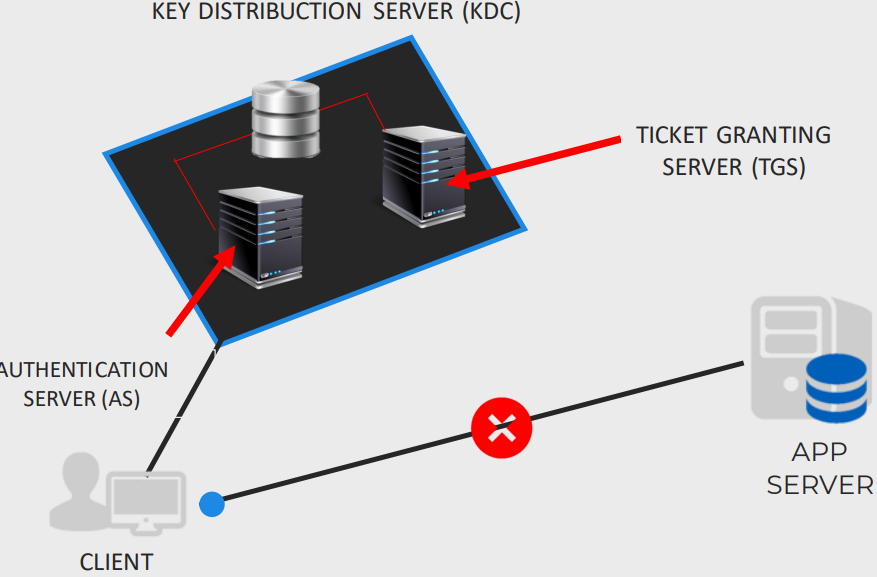
\includegraphics[keepaspectratio]{images/image43.png}}}

\paragraph{\texorpdfstring{{Step 2}}{Step 2}}\label{h.r85ttr597fdv}

{Arrivata la richiesta all'AS recupera la password del client nel Db
utilizzando lo username e }{decifra}{~l'intero msg verificando la sua
identità. Ed invia al client una risposta (KRB\_AS\_REP) che contiene: }

\begin{enumerate}
\tightlist
\item
  {Username client in chiaro }
\item
  {II TGT (Ticket Granting Ticket) cifrato con una secret key }
\item
  {User data AS cifrato con la user psw }
\end{enumerate}

{\pandocbounded{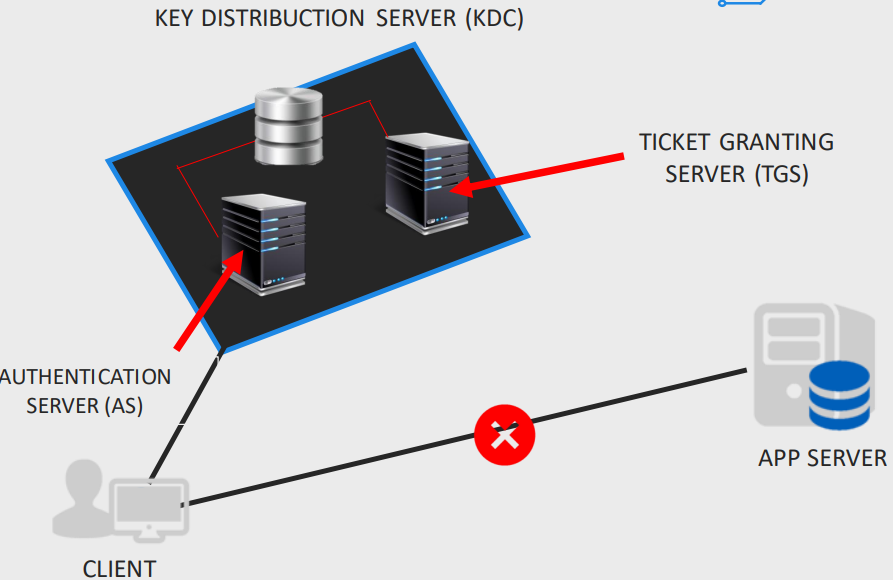
\includegraphics[keepaspectratio]{images/image61.png}}}

{Il TGT è formato da:}

\begin{itemize}
\tightlist
\item
  {Username client }
\item
  {Session key - Data di scadenza del TGT }
\item
  {PAC }{(Priviledge}{~Attribute Certificate) contenente le informazioni
  utili sui privilegi dell'utente }
\end{itemize}

{}

{User Data AS invece contiene: }

\begin{itemize}
\tightlist
\item
  {Session key }
\item
  {Data di scadenza del TGT }
\item
  {User nonce }
\end{itemize}

\paragraph{\texorpdfstring{{Step 3}}{Step 3}}\label{h.spuxtu1emcr6}

{Il }{client}{~avendo ricevuto il TGT procede inviando la richiesta
(KRB\_TGS\_REQ ) di accesso al servizio al TGS. }

{Tale richiesta sarà formata da:}

\begin{enumerate}
\tightlist
\item
  {~Username e timestamp cifrato con la session key }
\item
  {Il TGT così com è perchè non conosce la chiave per decifrarlo }
\item
  {User nonce }
\item
  {Nome del servizio richiesto(SPN)}
\end{enumerate}

\paragraph{\texorpdfstring{{Step 4}}{Step 4}}\label{h.u3bklls3fwgq}

{Il TGS ricevute le informazioni invia una risposta (KRB\_TGS\_REP ) al
}{Client}{~}{contenente:}

\begin{itemize}
\tightlist
\item
  {Username in chiaro }
\item
  {Il Ticket Granting Service cifrato con un'altra secret key }
\item
  {User Data TGS cifrate con la session key }
\end{itemize}

{Il Ticket Granting Service è formato da:}

\begin{itemize}
\tightlist
\item
  {~Username client - Service Session key }
\item
  {Data di scadenza del Ticket - PAC User Data TGS invece contiene: }
\item
  {Service Session key }
\item
  {Data di scadenza del Ticket }
\item
  {User nonce }
\end{itemize}

{}

{Il Client ricevuto Il Ticket Granting Service e interpretando la
service session key invia all'App Server la richiesta di accesso alla
risorsa (KRB\_AP\_REQ) che contiene:}

\begin{itemize}
\tightlist
\item
  {Ticket granting service che non può decifrare non conoscendo la
  chiave di decifratura }
\item
  {Username e Timestamp cifrate con la service session key}
\end{itemize}

{\pandocbounded{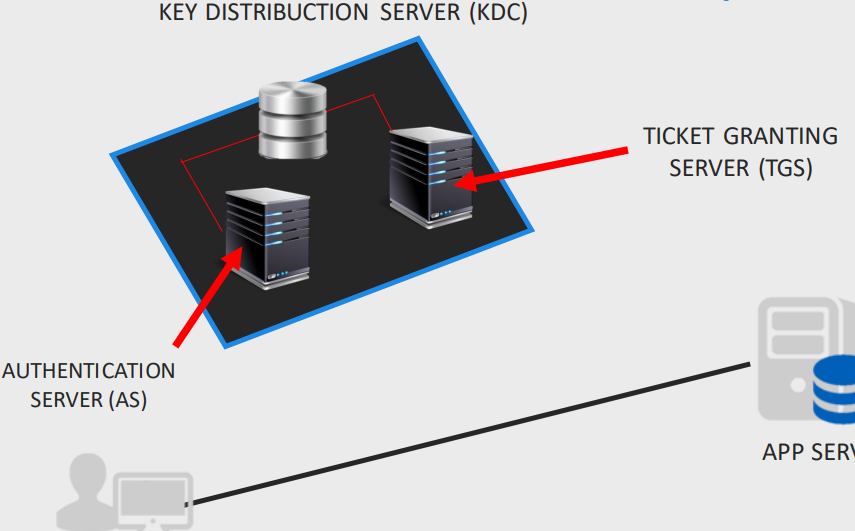
\includegraphics[keepaspectratio]{images/image119.png}}}

\paragraph{\texorpdfstring{{Step 5}}{Step 5}}\label{h.x4kkqztdewdi}

{L'App Server verifica il contenuto del Ticket Granting Service (più
precisamente interpreta il PAC) potendo decifrare entrambi in quanto è a
conoscenza di tutte le Secret Key essendo esse condivisa con il KDC. }

{E in caso di risposta affermativa dà il permesso al client di
utilizzare il servizio.}

{\pandocbounded{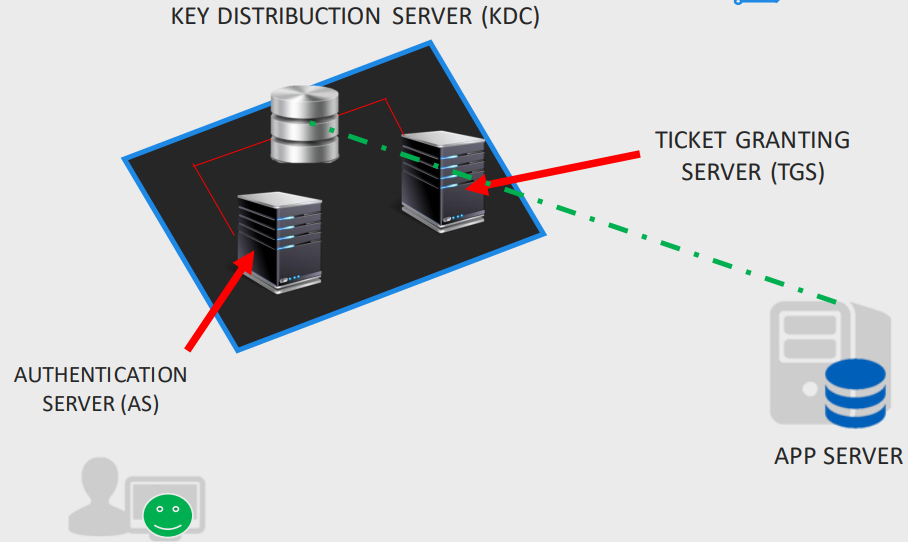
\includegraphics[keepaspectratio]{images/image25.png}}}

{}

{Per ricordare:}

{Key Distribution Center (KDC)}{~è la terza entità che verifica
l'identità e rilascia i TGT.}

{Comprende il TGS e AS.}

{}

{Ticket Granting Ticket (TGT) }{è il ticket che serve per accedere al
TGS e dimostrare che si è identificati.}

{}

{Ticket Granting }{Service}{~(TGS) }{convalida il TGT e rilascia un
ticket per accedere ad un servizio.}

\subsubsection{\texorpdfstring{{Vantaggi}}{Vantaggi}}\label{h.ybpr8qnnh74q}

\begin{itemize}
\tightlist
\item
  {Password}{~non vengono mai inviate in rete in formato testuale. }
\item
  {Le ``chiavi segrete'' sono trasmesse nel sistema solo in forma
  criptata. }
\item
  {Tracciamento di chi ha }{richiesto}{~che cosa e quando molto semplice
  }
\item
  {Il servizio permette inoltre agli utenti e ai sistemi di servizio di
  autenticarsi a vicenda. }
\item
  {A ogni passo del processo di autenticazione, sia gli utenti che i
  sistemi server sanno di avere a che fare con una controparte
  autentica.}
\end{itemize}

\subsubsection{\texorpdfstring{{Svantaggi}}{Svantaggi}}\label{h.d1ir5egkocqq}

\begin{itemize}
\tightlist
\item
  {Kerberoasting}{~}
\item
  {Golden Ticket e Silver Ticket }
\item
  {Le versioni più vecchie possono ancora essere utilizzate con la
  crittografia DES. }
\item
  {Replay attacks }
\end{itemize}

\subsection{\texorpdfstring{{Kerberoasting}}{Kerberoasting}}\label{h.vr59dm2w2e8}

{Kerberoasting}{~ci permette di decifrare le password degli account di
servizio per accedere a un dominio Active Directory come qualsiasi
utente autenticato.}

{Per farlo chiediamo al TGS ticket service (all'interno dell'Active
directory) per gli account di servizio specificando il loro valore SPN.
Quindi possiamo forzare questi ticket fino a quando non vengono violati,
senza alcun rischio di rilevamento o blocco
dell\textquotesingle account, ottenendo la password
dell\textquotesingle account.}

{}

{\href{https://www.google.com/url?q=https://virtuale.unibo.it/pluginfile.php/2023963/mod_resource/content/1/Laboratorio\%2520di\%2520sicurezza\%2520dei\%2520sistemi\%2520informatici\%2520e\%2520privacy\%2520-\%252002\%2520Active\%2520Directory\%2520Security\%2520-\%2520V1R0.pdf&sa=D&source=editors&ust=1734628852099535&usg=AOvVaw35pStrAiFzG1MzxltoITjS}{QUI
{[}37 - 41{]}}}

\subsection{\texorpdfstring{{Silver
Ticket}}{Silver Ticket}}\label{h.t2ow9l4zg9y1}

{Attacco che comporta la compromissione delle credenziali e
l\textquotesingle abuso del design del protocollo Kerberos. }

{Consente a un utente malintenzionato di falsificare i TGS per servizi
specifici. I Tickets sono crittografati con l\textquotesingle hash della
password per il servizio; pertanto, se un attaccante ruba
l\textquotesingle hash per un account di servizio, può creare TGS Ticket
per quel servizio. }

{}

{\href{https://www.google.com/url?q=https://virtuale.unibo.it/pluginfile.php/2023963/mod_resource/content/1/Laboratorio\%2520di\%2520sicurezza\%2520dei\%2520sistemi\%2520informatici\%2520e\%2520privacy\%2520-\%252002\%2520Active\%2520Directory\%2520Security\%2520-\%2520V1R0.pdf&sa=D&source=editors&ust=1734628852100089&usg=AOvVaw2uFr1HvAavHHCWtBTru8Pu}{QUI
{[}42 - 45{]}}}

\subsection{\texorpdfstring{{Golden
Ticket}}{Golden Ticket}}\label{h.4war67e8lxp9}

{Un Golden Ticket in Active Directory garantisce al beneficiario un
accesso illimitato alla risorsa tramite compromissione del protocollo
Kerberos.}

{}

{Avviene quando un attaccante compromette l\textquotesingle hash della
password KRBTGT, nota solo al Key Distribution Center (KDC), e la
utilizza per emettere i biglietti Kerberos riuscendo ad accedere a
qualsiasi risorsa desiderata.}

{}

{\href{https://www.google.com/url?q=https://virtuale.unibo.it/pluginfile.php/2023963/mod_resource/content/1/Laboratorio\%2520di\%2520sicurezza\%2520dei\%2520sistemi\%2520informatici\%2520e\%2520privacy\%2520-\%252002\%2520Active\%2520Directory\%2520Security\%2520-\%2520V1R0.pdf&sa=D&source=editors&ust=1734628852100528&usg=AOvVaw3wfNTIGS7jZbAknvTFwWZT}{QUI
{[}46 - 51{]}}}

{}

{La differenza principale tra un silver ticket e un golden ticket sta
nel livello di accesso che concedono a un utente non autorizzato.}

\begin{itemize}
\tightlist
\item
  {Golden Ticket}{: ticket di autenticazione Kerberos contraffatto che
  concede all\textquotesingle utente l\textquotesingle{}}{accesso a
  qualsiasi servizio nel dominio}{. Viene creato falsificando un
  Ticket-Granting Ticket (TGT), che è il ticket iniziale che un utente
  ottiene dal Kerberos Authentication Server (KDC) dopo
  l\textquotesingle autenticazione. Un golden ticket è come una chiave
  passepartout che apre qualsiasi porta nel dominio.}
\end{itemize}

{}

\begin{itemize}
\tightlist
\item
  {Silver Ticket}{: ticket di autenticazione Kerberos contraffatto che
  concede all\textquotesingle utente l\textquotesingle accesso }{solo a
  un servizio specifico nel dominio}{. Viene creato falsificando un
  Ticket-Granting }{Service}{~(TGS) ticket, che è il ticket che un
  utente ottiene dal KDC per accedere a un servizio specifico. Un silver
  ticket è come una chiave contraffatta che apre solo una porta
  specifica nel dominio.}
\end{itemize}

{}

\section{\texorpdfstring{{Sicurezza applicativi
web}}{Sicurezza applicativi web}}\label{h.dx6gakjh42r2}

{\pandocbounded{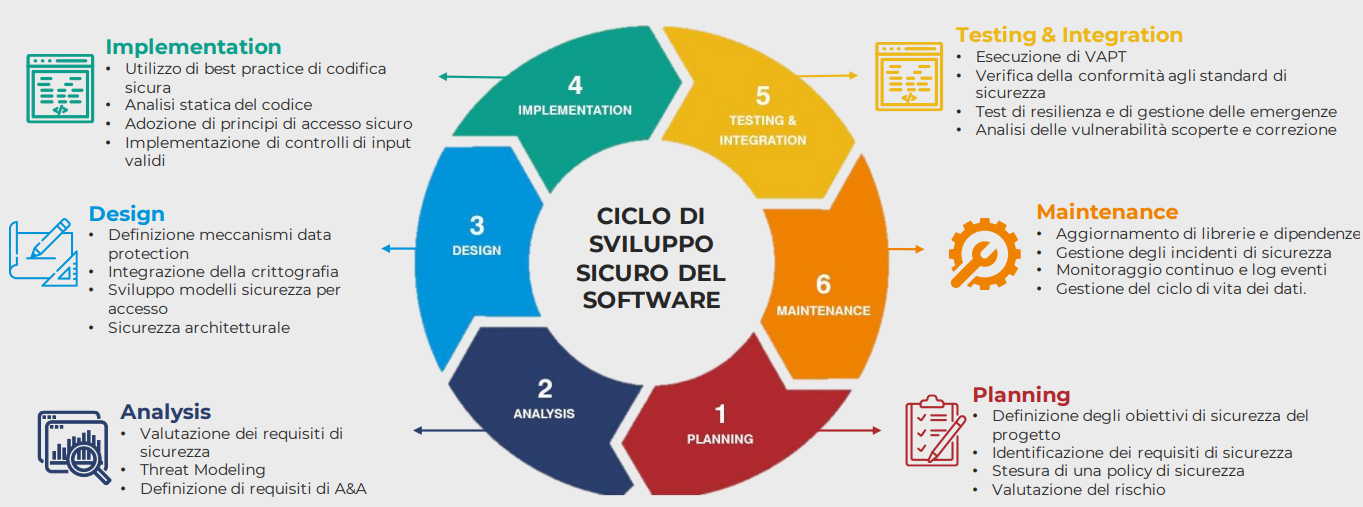
\includegraphics[keepaspectratio]{images/image105.png}}}

{La sicurezza va valutata in ogni fase non solo nell'implementazione.}

\subsection{\texorpdfstring{{Standard}}{Standard}}\label{h.ruwx391qdpb2}

{Ora vediamo una carrellata di standard di riferimento:}

\begin{itemize}
\tightlist
\item
  {CERT Secure Coding Standard}{: sviluppato appunto dal CERT e fra i
  vari principi si occupa di:}
\end{itemize}

\begin{itemize}
\tightlist
\item
  {prevenzione delle vulnerabilità;}
\item
  {input validation (per }{evitare}{~SQL injection) quindi controllo
  dell'input client/server side;}
\item
  {sicurezza comunicazioni;}
\end{itemize}

\begin{itemize}
\tightlist
\item
  {SSDF - Secure Software Development Framework}{: del NIST è un quadro
  di riferimento completo per garantire la sicurezza del software
  durante tutto il ciclo di sviluppo mostrato sopra, con enfasi sulla
  fase di progettazione;}
\item
  {PCI DSS - Payment Card Industry Data Security}{: che dice come il
  software deve essere gestito per garantire un pagamento in rete
  sicuro;}
\item
  {OWASP Application Security verification Standard}{: è un }{framework
  + standard}{~di sicurezza progettato per valutare delle applicazioni
  web e dei servizi web.}
\end{itemize}

\subsection{\texorpdfstring{{Best
practice}}{Best practice}}\label{h.5q5oypnm3p8m}

\subsubsection{\texorpdfstring{{Deny by
default}}{Deny by default}}\label{h.tqnw2pq3lpoq}

{Per accedere ad una determinata risorsa devi essere in whitelist,
quindi di base nessuno può accedere ed è il gestore che da il permesso a
ciascun individuo.}

\subsubsection{\texorpdfstring{{Least privilege
principle}}{Least privilege principle}}\label{h.mq3savs7b3ws}

{Si riducono al minimo i privilegi di ogni utente per evitare che chi
non di dovere vada ad accedere a parti sensibili.}

\subsubsection{\texorpdfstring{{Defense in
Depth}}{Defense in Depth}}\label{h.wb61oa88bus0}

{Il principio è di mettere una sicurezza in più livelli in modo da
fermare un malintenzionato molto prima}

{\pandocbounded{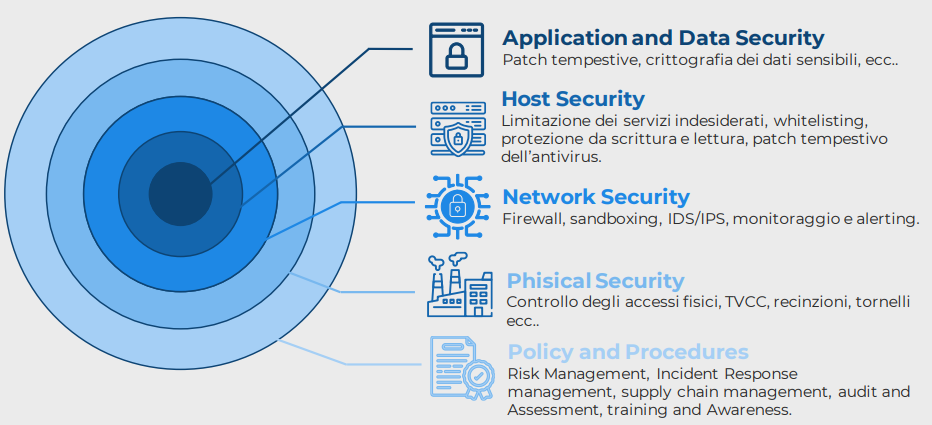
\includegraphics[keepaspectratio]{images/image35.png}}}

\subsubsection{\texorpdfstring{{Validate
input}}{Validate input}}\label{h.lpp5rzin7zu6}

{Consiste nel verificare e garantire che i dati inseriti in
un\textquotesingle applicazione rispettino determinati criteri e
regole.}

{La mancanza di una corretta validazione dell\textquotesingle input può
portare a vulnerabilità di sicurezza, quali attacchi di injection, e
compromettere l\textquotesingle integrità e la funzionalità
dell\textquotesingle applicazione. }

{}

{Contiene la data sanitization.}

\subsubsection{\texorpdfstring{{Compiler
Warnings}}{Compiler Warnings}}\label{h.6641qng6302v}

{I "compiler warnings" sono avvertimenti emessi durante la compilazione
del codice per segnalare possibili problemi o pratiche di programmazione
rischiose. }

{Fondamentali per garantire la sicurezza del software, spesso questi
messaggi identificano potenziali vulnerabilità, come
l\textquotesingle uso di variabili non inizializzate o conversioni di
tipo insicure, che potrebbero essere sfruttate in attacchi informatici.
}

\subsubsection{\texorpdfstring{{KISS}}{KISS}}\label{h.2lhn1uftxvo9}

{Acronimo che sta per ``Keep It Simple, Stupid'' che promuove la
scrittura di codice semplice e diretto senza complessità non
necessaria.}

\subsubsection{\texorpdfstring{{Data
Sanitization}}{Data Sanitization}}\label{h.f03jvneprplf}

{Pulizia e validazione di dati per prevenire attacchi informatici.}

{Questo implica l\textquotesingle uso di tecniche come
l\textquotesingle escape dei caratteri speciali, la validazione dei
formati, il filtraggio dei caratteri pericolosi e
l\textquotesingle implementazione di query parametrizzate nei database.}

\subsection{\texorpdfstring{{OWASP
}{TOP10}}{OWASP TOP10}}\label{h.ndnn9nbby4sx}

{Comunità dedicata a indirizzare le organizzazioni nel sviluppare,
acquistare e mantenere applicazioni e API affidabili e sicure. }

{Tutti gli strumenti, i documenti, i video, le presentazioni e i
capitoli di OWASP sono gratuiti e aperti a chiunque sia interessato a
migliorare la sicurezza delle applicazioni. }

{La fondazione OWASP è l\textquotesingle ente no-profit che garantisce
il successo a lungo termine del progetto}

{}

{Nel 2021 OWASP ha stilato una top 10 dei rischi di sicurezza più
problematici}

{\pandocbounded{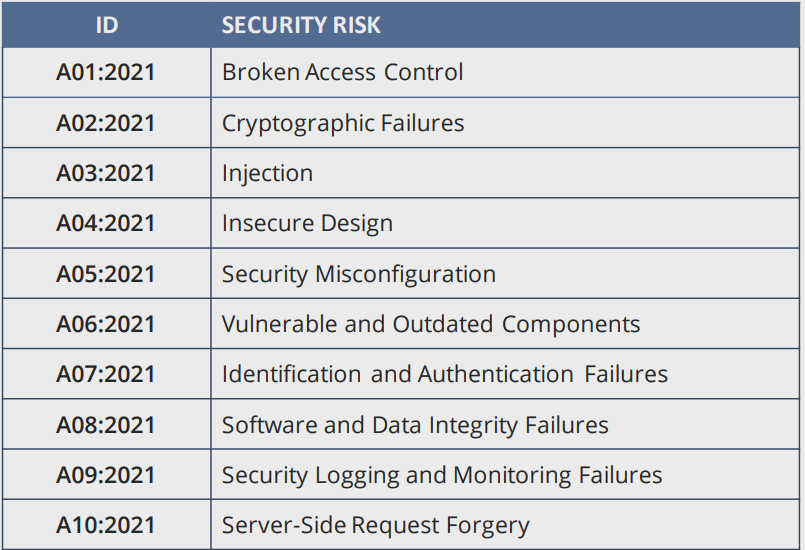
\includegraphics[keepaspectratio]{images/image12.png}}}

\subsubsection{\texorpdfstring{{Broken Access
Control}}{Broken Access Control}}\label{h.h24np3y3z3yy}

{Il Broken Access Control si contestualizza all\textquotesingle interno
del processo di verifica dell\textquotesingle identità e della liceità
delle richieste, denominato controllo degli accessi e si concretizza
nella sua elusione o, comunque, nella modifica dei controlli
inizialmente implementati.}

{}

{\pandocbounded{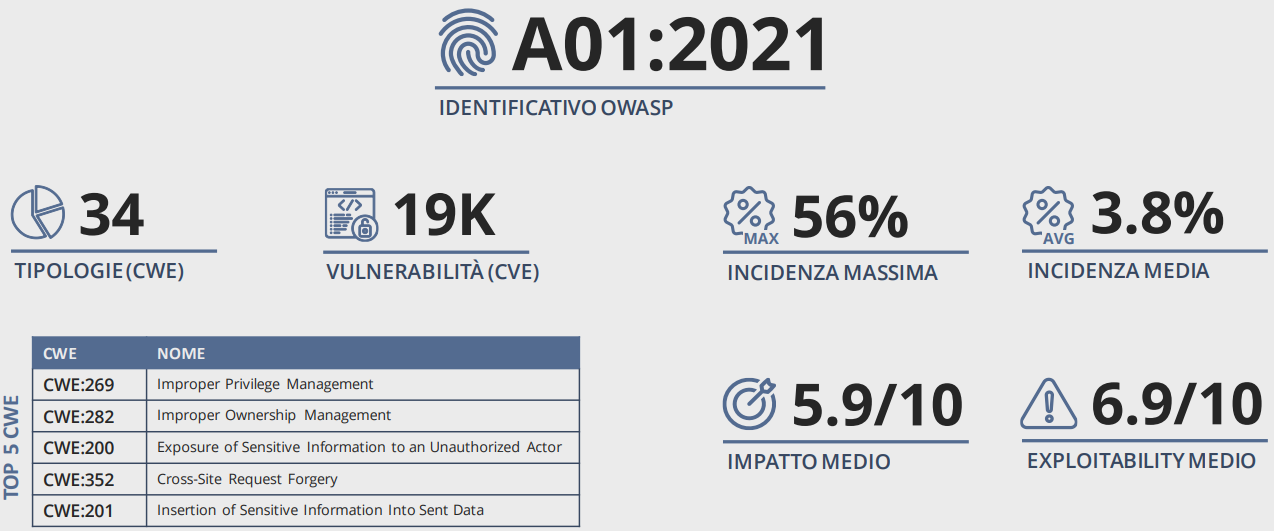
\includegraphics[keepaspectratio]{images/image85.png}}}

{Le tipologie }{CWE}{~sono le categorie di vulnerabilità CVE trovati.}

{L'incidenza indica quanti applicativi (nel pool analizzato) sono
vulnerabili a questa falla.}

{L'impatto medio delle vulnerabilità sull'applicativo.}

{L'exploitability}{~medio è quanto è facile sfruttare le vulnerabilità.}

{}

{Alcune nozioni per capire meglio la vulnerabilità:}

{\pandocbounded{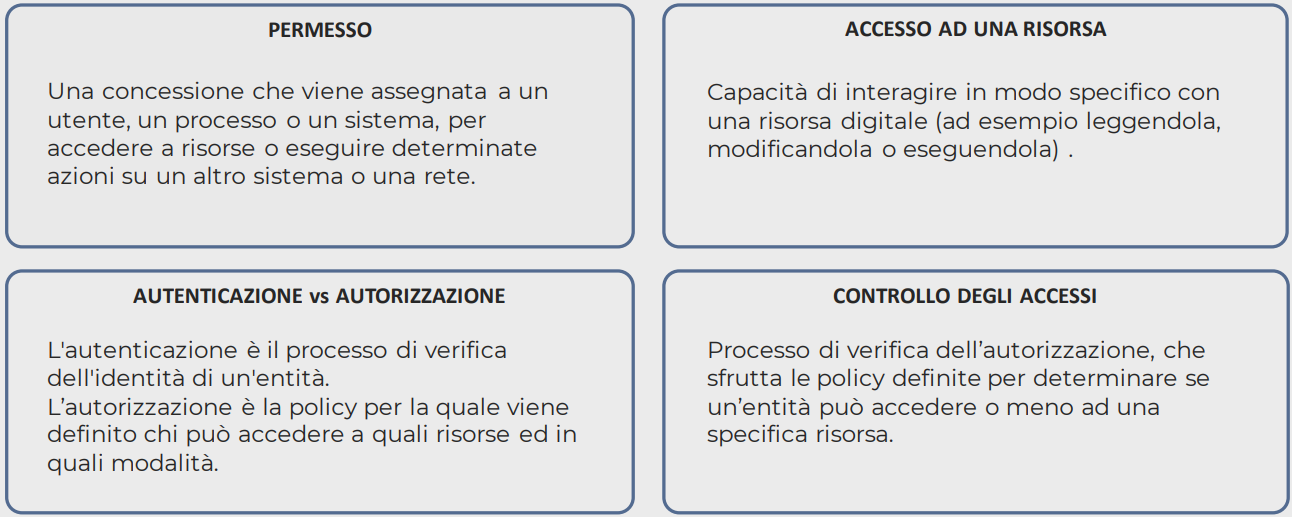
\includegraphics[keepaspectratio]{images/image19.png}}}

{Il controllo degli accessi serve a garantire che gli utenti rispettino
le regole stabilite, impedendo loro di compiere azioni non
consentite.Quando ci sono problemi con questo tipo di controllo, possono
verificarsi situazioni indesiderate come la divulgazione non autorizzata
di informazioni, la manipolazione o la distruzione dei dati, oppure
l\textquotesingle esecuzione di funzioni aziendali al di là dei permessi
dell\textquotesingle utente. Bisogna stare attenti che le risorse che
difendiamo non siano accessibili da altri canali rendendo inutile il
controllo}

{}

{}

{}

{La definizione formale è:}

{Il Broken Access Control è una categoria di vulnerabilità ampiamente
riscontrata in sistemi software, includendo anche applicativi Web, che
consiste in problemi legati ai permessi di accesso, aventi impatto sulla
sicurezza di sistemi, processi e informazioni. }

{}

{Nella tabella le principali contromisure riguardo broken access
control:}

{\pandocbounded{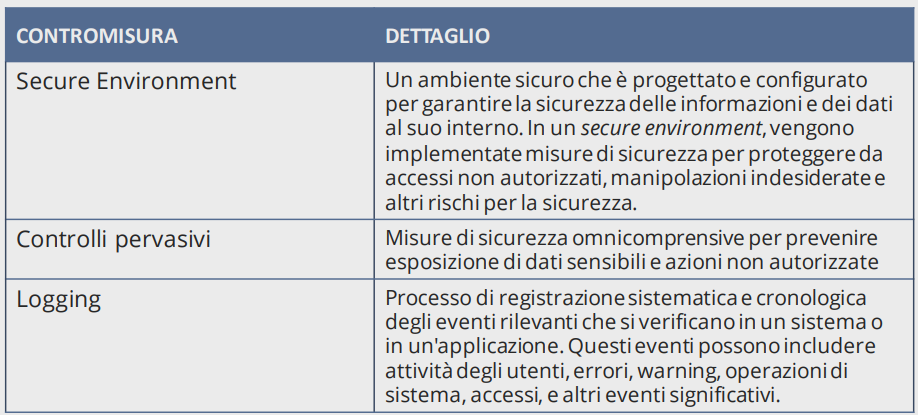
\includegraphics[keepaspectratio]{images/image81.png}}}{\pandocbounded{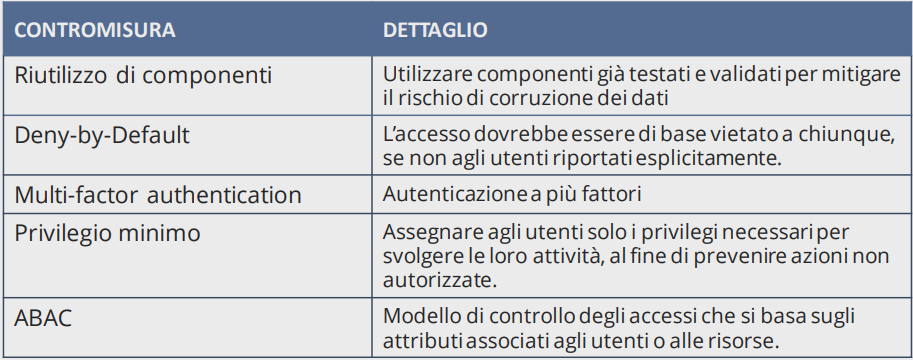
\includegraphics[keepaspectratio]{images/image11.png}}}

{\pandocbounded{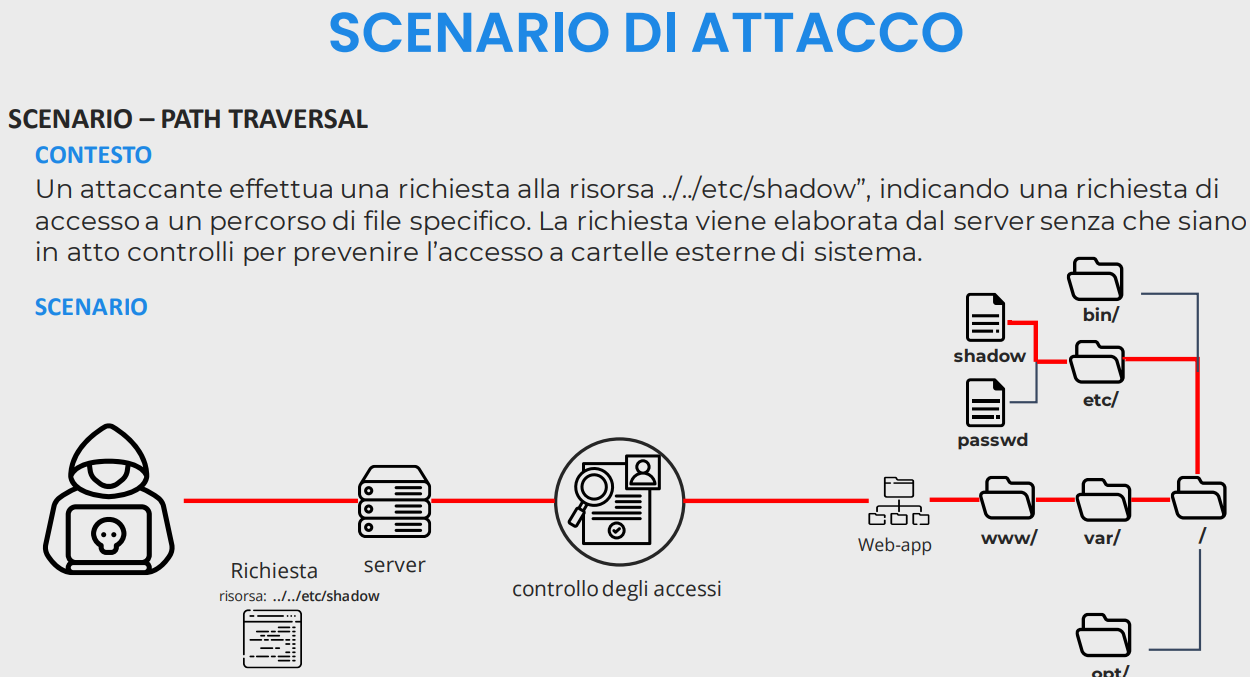
\includegraphics[keepaspectratio]{images/image30.png}}}

{In conclusione:}

{}

{Il Broken Access Control è, ad oggi, un rischio significativo. }

{}

{Per evitarlo, è cruciale seguire best practice di sicurezza durante
l\textquotesingle intero ciclo di vita del software, comprese le fasi di
analisi, progettazione e implementazione. }

{È essenziale applicare principi come il privilegio minimo e
implementare un sistema solido di controllo degli accessi basato su
profili autorizzativi. }

{}

{L\textquotesingle identificazione e l\textquotesingle autenticazione
sicure sono misure fondamentali per garantire
l\textquotesingle efficacia dei processi autorizzativi. Validazioni
robuste, eseguite sia lato client sia lato server, verificate ad ogni
richiesta, risultano fondamentali.}

\subsubsection{\texorpdfstring{{Cryptographic
failures}}{Cryptographic failures}}\label{h.w9ku64qfskat}

{I dati sensibili potrebbero essere esposti in diversi modi, tra questi
spiccano implementazioni crittografiche errate in modo parziale o
totale. }

{Errori legati alla crittografia spesso portano, infatti,
all\textquotesingle esposizione di dati sensibili o addirittura alla
compromissione del sistema, sia al momento della memorizzazione delle
informazioni, sia al momento dell'invio.}

{\pandocbounded{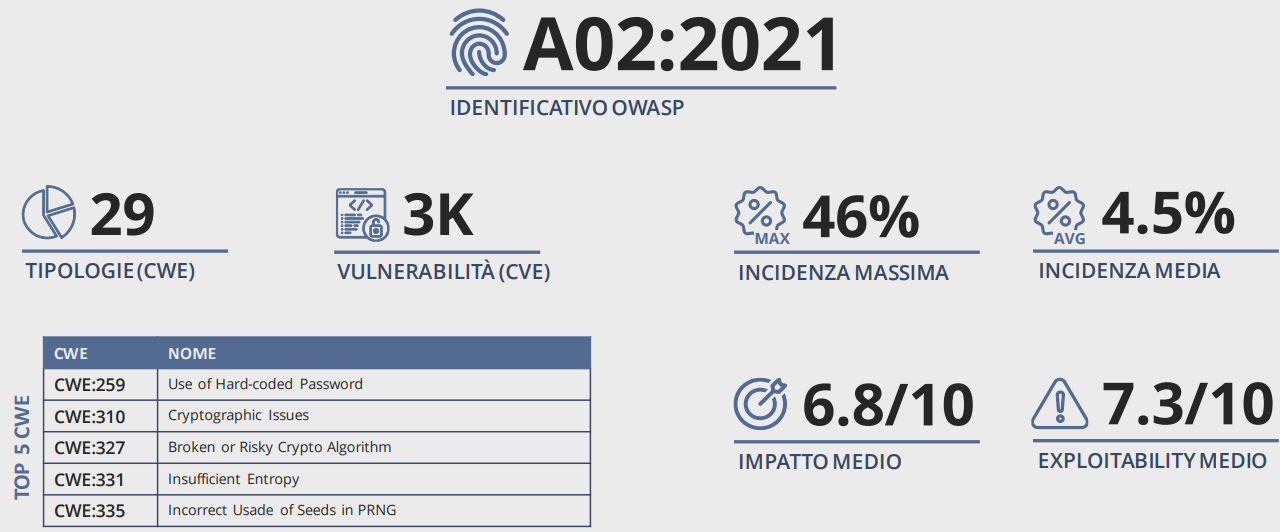
\includegraphics[keepaspectratio]{images/image82.png}}}

{}

{Alcune nozioni per capire meglio la vulnerabilità:}

{\pandocbounded{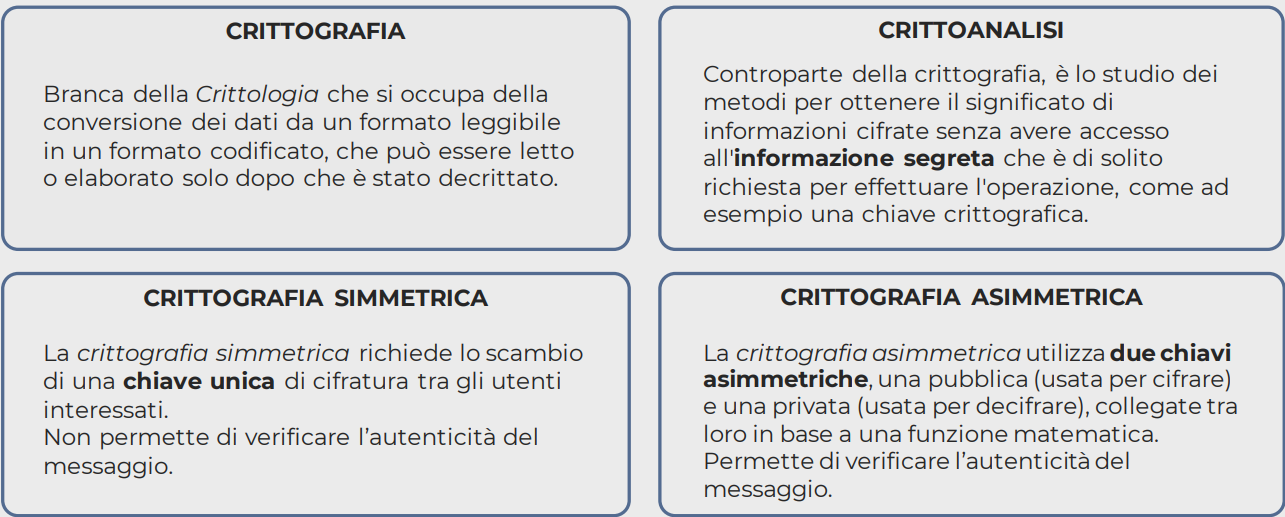
\includegraphics[keepaspectratio]{images/image20.png}}}

{}

{La definizione è:}

{Il Cryptographic Failures è una categoria di debolezze ampiamente
riscontrata in sistemi software, includendo anche applicativi web, che
consiste in problemi nella progettazione,
nell\textquotesingle implementazione o nell'uso di algoritmi e
protocolli crittografici, che causano impatti nella sicurezza di
sistemi, processi e informazioni.}

{}

{Il Cryptographic Failures di OWASP fornisce una guida dettagliata sugli
errori crittografici più comuni e pericolosi che possono verificarsi
nell\textquotesingle implementazione di funzionalità crittografiche
all\textquotesingle interno di un\textquotesingle applicazione, i
principali sono:}

\begin{itemize}
\tightlist
\item
  {~Algoritmi crittografici deboli o insicuri: l\textquotesingle uso di
  algoritmi crittografici deboli o obsoleti può compromettere la
  sicurezza di un sistema. Ad esempio, l\textquotesingle impiego di
  algoritmi come DES o MD5 è considerato insicuro. }
\end{itemize}

{}

\begin{itemize}
\tightlist
\item
  {Problemi nella generazione e gestione delle chiavi: errori nella
  generazione, gestione o protezione delle chiavi crittografiche possono
  portare a vulnerabilità significative. }
\end{itemize}

{}

\begin{itemize}
\tightlist
\item
  {Utilizzo improprio della crittografia: implementazione erronea della
  crittografia, come l\textquotesingle uso di modalità insicure o la
  mancata applicazione di funzioni di hashing, può compromettere la
  protezione dei dati. }
\end{itemize}

{}

\begin{itemize}
\tightlist
\item
  {Mancanza di controllo dell'integrità dei dati: assenza di meccanismi
  per verificare l\textquotesingle integrità dei dati crittografati può
  consentire attacchi di manipolazione. }
\end{itemize}

{}

\begin{itemize}
\tightlist
\item
  {Problemi di implementazione del protocollo: errori
  nell\textquotesingle implementazione di protocolli crittografici, come
  TLS/SSL, possono portare all'esposizione totale di dati sensibili.}
\end{itemize}

{}

{Nella tabella le principali contromisure riguardo cryptographic
failures:}

{\pandocbounded{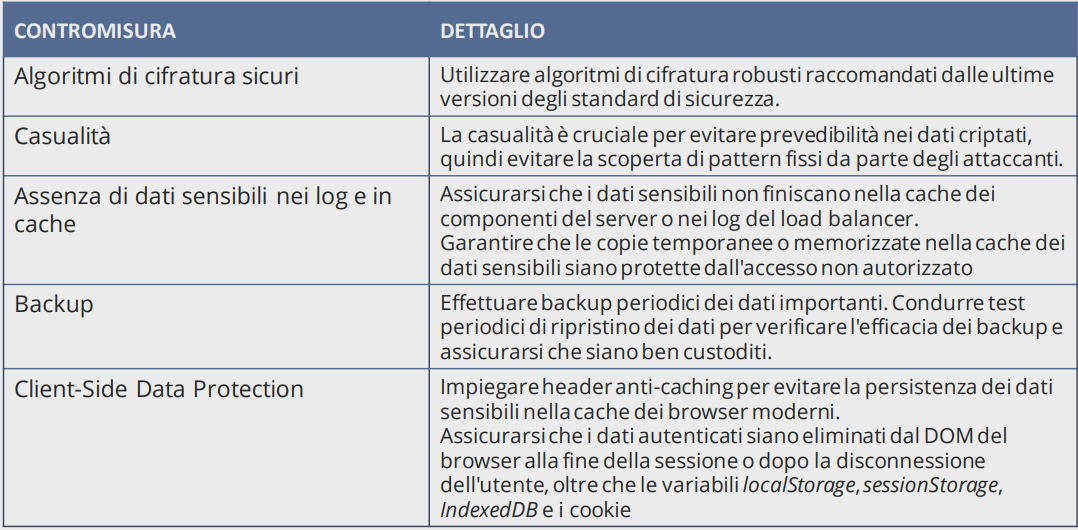
\includegraphics[keepaspectratio]{images/image51.png}}}

{\pandocbounded{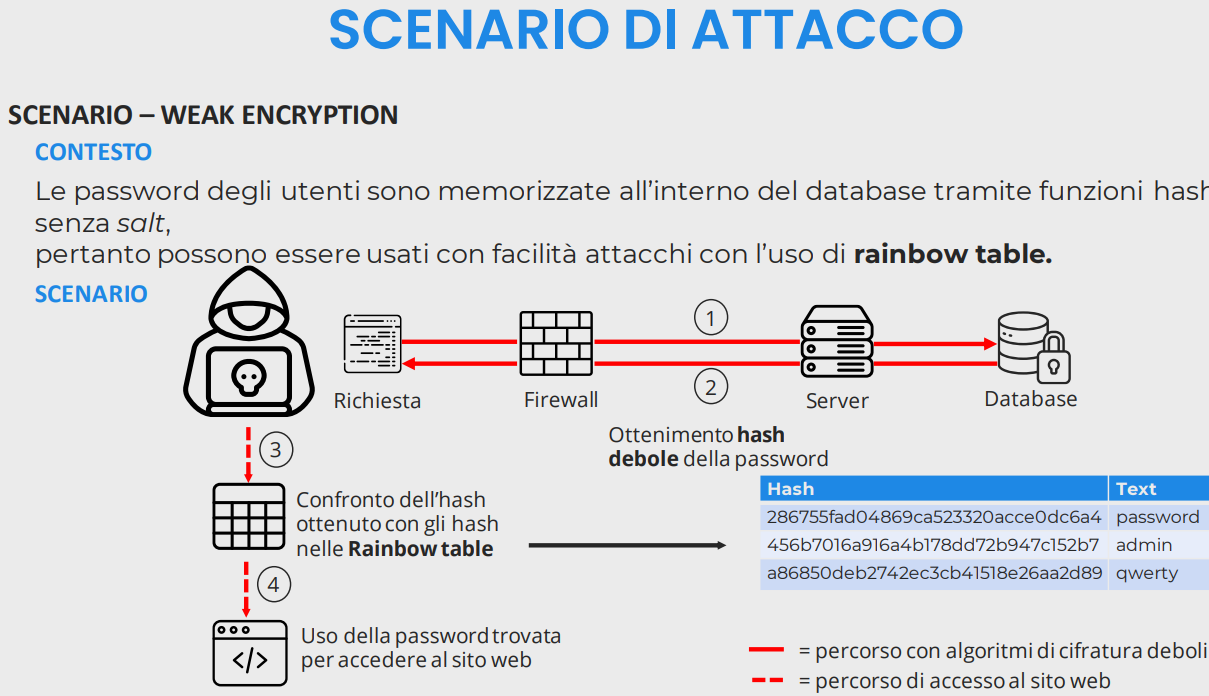
\includegraphics[keepaspectratio]{images/image103.png}}}

{}

{In conclusione:}

{}

{Il Cryptographic Failures rappresenta una delle minacce più rilevanti e
pervasive nell\textquotesingle ambito della sicurezza delle applicazioni
Web. La crittografia svolge un ruolo cruciale nella protezione dei dati
sensibili e nella garanzia dell\textquotesingle integrità delle
comunicazioni, ma errori nella sua implementazione possono comportare
gravi conseguenze. }

{}

{Il Cryptographic Failures può mettere a rischio la confidenzialità dei
dati e la sicurezza delle applicazioni. }

\subsubsection{\texorpdfstring{{Injection}}{Injection}}\label{h.wxfqtl7d7b7x}

{Le vulnerabilità di tipo injection vedono la loro causa primaria nella
gestione }{incorretta}{~dei dati di input. }

{Gli attacchi di tipo injection si differenziano in base alla tecnologia
colpita e alle modalità di esecuzione dell'attacco (SQL injection, OS
command injection, Cross Site Scripting (XSS)). }

{\pandocbounded{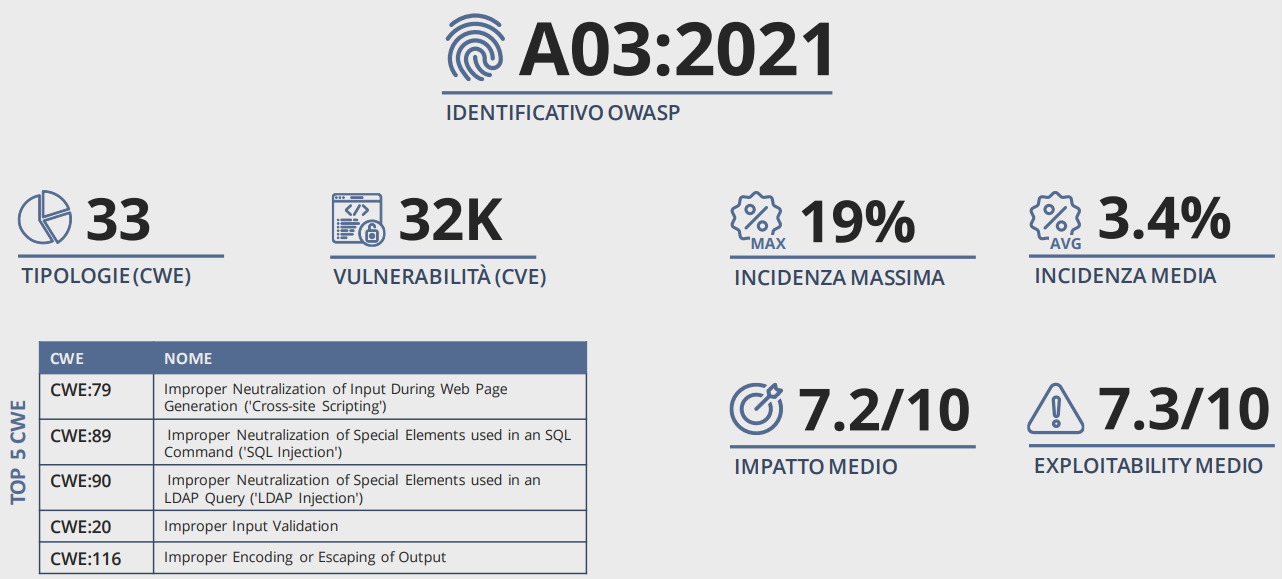
\includegraphics[keepaspectratio]{images/image89.png}}}

{}

{Alcune nozioni per capire meglio la vulnerabilità:}

{\pandocbounded{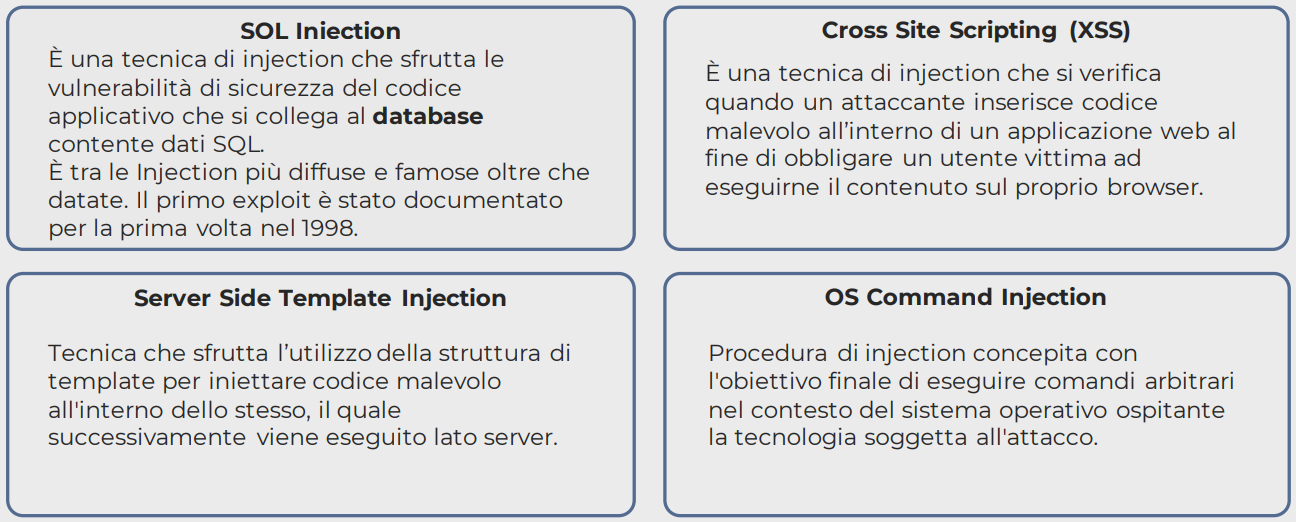
\includegraphics[keepaspectratio]{images/image7.png}}}

{}

{La definizione è:}

{L\textquotesingle Injection è una tecnica di attacco informatico che
consiste nell'inserimento di codice malevolo in un'applicazione, in un
processo in esecuzione o in un database, al fine di modificarne il
comportamento previsto.}

{}

{}

{Gli attacchi di tipo injection, variegati e strettamente legati alla
tecnologia coinvolta, condividono il concetto fondamentale: manipolare
la logica di esecuzione dell\textquotesingle applicativo attraverso
l\textquotesingle inserimento di input controllato
dall\textquotesingle utente malintenzionato.}

{}

{Ad esempio, i buffer overflow sfruttano l\textquotesingle inserimento
di una quantità eccessiva di dati per sovrascrivere parti del codice,
potenzialmente compromettendo il servizio e permettendo
l\textquotesingle esecuzione di codice malevolo. La radice del problema
risiede nella mancanza di controlli sull\textquotesingle input; è
essenziale verificarne la conformità alle aspettative e considerare non
valido l\textquotesingle input non conforme.}

{}

{}

{}

{}

{}

{}

{Nella tabella le principali contromisure riguardo injection:}

{\pandocbounded{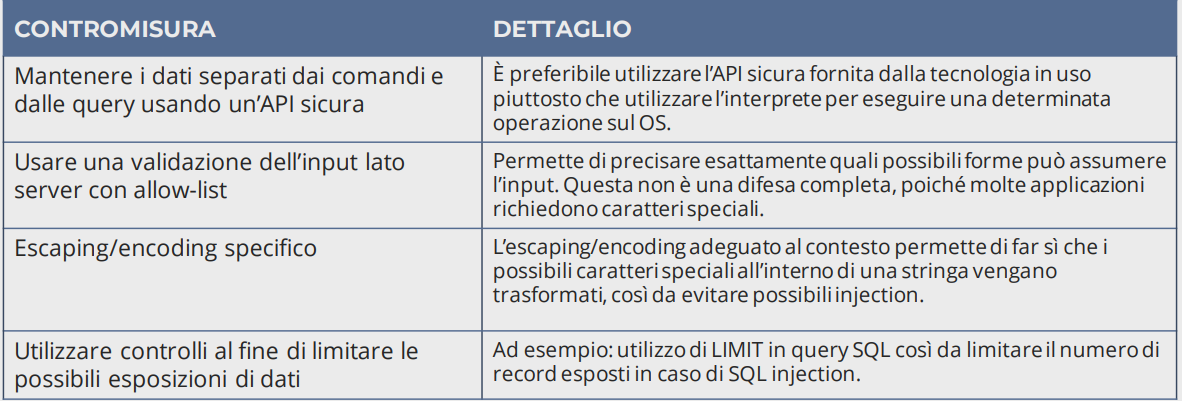
\includegraphics[keepaspectratio]{images/image91.png}}}

{}

{\pandocbounded{\includegraphics[keepaspectratio]{images/image95.png}}}

\subsubsection{\texorpdfstring{{Insecure
design}}{Insecure design}}\label{h.9eummayphlf9}

{Si concentra sui rischi associati ai difetti di progettazione e
architetturali. In particolare, questa categoria si dedica al threat
modeling, all\textquotesingle utilizzo di design-pattern sicuri e alle
scelte architetturali. }

{Uno dei fattori che contribuisce all'insecure design è la mancanza di
un profilo di rischio a livello di business, che comporta una carenza di
conoscenza dei livelli di sicurezza necessari. }

{Un design insicuro rimane vulnerabile anche in assenza di bug, poiché
per sua natura manca delle protezioni necessarie a livello progettuale.
Le conseguenze di una possibile falla nel design dipendono fortemente
dall\textquotesingle origine del problema, ovvero dalla mancanza a
livello progettuale. Tali conseguenze possono tradursi in ingenti
perdite economiche, poiché risolvere una lacuna a livello progettuale
richiede uno sforzo significativo.}

{\pandocbounded{\includegraphics[keepaspectratio]{images/image66.png}}}

{}

{Alcune nozioni per capire meglio la vulnerabilità:}

{\pandocbounded{\includegraphics[keepaspectratio]{images/image84.png}}}

{}

{La definizione è:}

{L\textquotesingle Insecure Design si riferisce a un approccio di
progettazione che presenta vulnerabilità e lacune nella sicurezza di un
sistema, applicazione o prodotto. Questo tipo di design manca di
controlli e misure di sicurezza efficaci, aumentando il rischio di
esposizione a minacce informatiche e violazioni della sicurezza.}

{}

{Nella tabella le principali contromisure riguardo insecure design:}

{\pandocbounded{\includegraphics[keepaspectratio]{images/image50.png}}}

{\pandocbounded{\includegraphics[keepaspectratio]{images/image106.png}}}

\subsubsection{\texorpdfstring{{Security
misconfiguration}}{Security misconfiguration}}\label{h.cuc39lb8grzg}

{la Security Misconfiguration, circa il 90\% di applicazioni testate
sono risultate vulnerabili ad essa. Non sorprende vedere questa
categoria così rilevante, essendo i software sempre più configurabili e,
spesso, lasciati dall'utente allo stato di default.}

{\pandocbounded{\includegraphics[keepaspectratio]{images/image15.png}}}

{\pandocbounded{\includegraphics[keepaspectratio]{images/image78.png}}}

{}

{La definizione è:}

{La Security Misconfiguration è una categoria di vulnerabilità che si
verifica quando un\textquotesingle applicazione, un server o qualsiasi
componente di un sistema è configurato in modo errato, lasciando aperte
vulnerabilità che potrebbero essere sfruttate dagli aggressori.}

{}

{Tali configurazioni di sicurezza errate possono manifestarsi in vari
modi, ad esempio: }

\begin{itemize}
\tightlist
\item
  {Permissive Configurations: Assegnare permessi eccessivi o non
  necessari a utenti, processi o risorse, consentendo
  l\textquotesingle accesso non autorizzato o il potenziale sfruttamento
  di vulnerabilità. }
\item
  {Insecure Defaults: Utilizzare impostazioni di default che sono
  intrinsecamente insicure. Ciò potrebbe includere password deboli,
  configurazioni di crittografia insoddisfacenti o altre scelte di
  configurazione che rendono il sistema vulnerabile. }
\item
  {Exposed Sensitive Information: Rivelare informazioni sensibili o
  dettagli implementativi nel codice, nei file di configurazione o
  altrove. Queste informazioni potrebbero essere sfruttate dagli
  aggressori per pianificare e condurre attacchi più mirati.}
\end{itemize}

{}

{Nella tabella le principali contromisure riguardo la security
misconfiguration:}

{\pandocbounded{\includegraphics[keepaspectratio]{images/image117.png}}}

{\pandocbounded{\includegraphics[keepaspectratio]{images/image97.png}}}

{}

{La Security Misconfiguration è una delle principali minacce alla
sicurezza delle applicazioni Web e dei sistemi in generale. Gli
attaccanti possono sfruttare configurazioni errate per ottenere accesso
non autorizzato, eseguire attacchi di traversing directory, scoprire
informazioni sensibili e altro ancora.}

{~È essenziale eseguire regolarmente audit di sicurezza e revisioni
delle configurazioni per identificare e correggere eventuali
vulnerabilità di configurazione.}

{}

\subsubsection{\texorpdfstring{{Vulnerable and outdated
components}}{Vulnerable and outdated components}}\label{h.z8cnea69mh4u}

{La categoria Vulnerable and Outdated Components di OWASP riguarda una
problematica nota, per la quale risulta complesso effettuare dei test
mirati e, }{pertanto calcolarne}{~il rischio.}

{}

{È infatti l'unica categoria per cui non è associato nessun Common
Vulnerability and Exposure (CVE).}

{\pandocbounded{\includegraphics[keepaspectratio]{images/image118.png}}}

{}

{\pandocbounded{\includegraphics[keepaspectratio]{images/image116.png}}}

{}

{La definizione è: }

{Il Vulnerable and Outdated Components è una minaccia alla sicurezza che
si verifica quando un\textquotesingle applicazione utilizza componenti
software, come librerie o framework, che contengono vulnerabilità di
sicurezza note o sono datati e non più supportati. }

{}

{Si vuole sottolineare, inoltre, che le applicazioni spesso dipendono da
componenti di terze parti per funzionare in modo efficiente. Tali
componenti potrebbero contenere vulnerabilità di sicurezza o potrebbero
essere obsolete. In tal caso, possono costituire una potenziale via di
accesso per gli attaccanti. Gli aggressori possono sfruttare le
vulnerabilità nelle versioni obsolete o noti problemi di sicurezza nelle
componenti utilizzate per compromettere l\textquotesingle applicazione
e, in ultima analisi, il sistema sottostante.}

{}

{Il Vulnerable and Outdated Components di OWASP si presenta se: }

\begin{itemize}
\tightlist
\item
  {Non si conoscono le versioni di tutti i componenti utilizzati (sia
  lato client che lato server). Questo include i componenti utilizzati
  direttamente così come le dipendenze annidate. }
\item
  {Se il software è vulnerabile, non supportato o non aggiornato. Questo
  include i sistemi operativi, i server web, i database management
  system (DBMS), le applicazioni, API e tutti i componenti, ambienti di
  esecuzione e librerie. }
\item
  {In caso non venissero effettuate scansioni periodiche di sicurezza e
  non si }{consultassero}{~i bollettini di sicurezza relativi ai
  componenti utilizzati. }
\item
  {In caso non fosse previsto un piano efficace di patch management
  relativamente alla piattaforma sottostante, i framework, e le
  dipendenze in modo tempestivo e basato sul rischio. }
\item
  {In assenza di test di specifici per verificare la non regressione del
  software a seguito di aggiornamenti di librerie.}
\end{itemize}

{}

{Nella tabella alcune contromisure:}

{\pandocbounded{\includegraphics[keepaspectratio]{images/image63.png}}}

\subsubsection{\texorpdfstring{{Identification and authentication
failures}}{Identification and authentication failures}}\label{h.442xo4lr9yda}

{Precedentemente denominata Broken Authentication. Questo termine si
riferisce a una serie di vulnerabilità e inefficienze che possono
emergere nei processi di identificazione e autenticazione, i quali sono
fondamentali per garantire l\textquotesingle accesso sicuro e
autorizzato ai sistemi e alle applicazioni.}

{\pandocbounded{\includegraphics[keepaspectratio]{images/image94.png}}}

{\pandocbounded{\includegraphics[keepaspectratio]{images/image2.png}}}

{}

{La definizione è: }

{Identification and Authentication Failures riguarda situazioni in cui i
meccanismi di autenticazione e identificazione di
un\textquotesingle applicazione non sono implementati in modo sicuro o
sono vulnerabili. Questo può includere problemi come la gestione
inadeguata delle sessioni, l\textquotesingle uso debole di password, la
mancanza di controlli di autenticazione multi-fattore, errori nelle
risposte di autenticazione e altri problemi legati
all\textquotesingle identificazione e alla verifica delle identità degli
utenti. }

{}

{Nella tabella alcune contromisure:}

{\pandocbounded{\includegraphics[keepaspectratio]{images/image107.png}}}

{\pandocbounded{\includegraphics[keepaspectratio]{images/image5.png}}}

\subsubsection{\texorpdfstring{{Software and data integrity
failures}}{Software and data integrity failures}}\label{h.en7rhlw4us9i}

{Si focalizza sulle relazioni di fiducia senza verifiche di integrità in
contesti di aggiornamento software, gestione di dati critici e CI/CD
pipelines.}

{\pandocbounded{\includegraphics[keepaspectratio]{images/image8.png}}}

{\pandocbounded{\includegraphics[keepaspectratio]{images/image22.png}}}

{}

{La definizione è:}

{La classe di vulnerabilità Software and Data Integrity Failures secondo
i dati forniti è caratterizzata da situazioni in cui il codice e
l\textquotesingle infrastruttura non proteggono adeguatamente contro
violazioni dell\textquotesingle integrità del software e dei dati. }

{}

{Queste vulnerabilità possono derivare da pratiche come
l\textquotesingle inclusione di funzionalità da fonti non attendibili,
la mancanza di verifica dell\textquotesingle integrità durante gli
aggiornamenti del software, e la presenza di vulnerabilità di
deserializzazione non sicura.}

{}

{Nella tabella alcune contromisure:}

{\pandocbounded{\includegraphics[keepaspectratio]{images/image65.png}}}

{\pandocbounded{\includegraphics[keepaspectratio]{images/image42.png}}}

{\pandocbounded{\includegraphics[keepaspectratio]{images/image98.png}}}

{}

{La gestione delle vulnerabilità di software e integrità dei dati
richiede un approccio strategico. L\textquotesingle implementazione di
firme digitali, controlli di accesso e la verifica delle dipendenze sono
essenziali per mitigare rischi come l\textquotesingle esecuzione di
codice malevolo o la compromissione dei dati. }

{}

{Processi di revisione e monitoraggio continuo sono fondamentali per
individuare e correggere potenziali vulnerabilità.
L\textquotesingle adozione di pratiche sicure nella catena di
distribuzione del software, inclusa la protezione delle pipeline CI/CD,
contribuisce a prevenire accessi non autorizzati e modifiche
indesiderate. }

{}

{Mantenere le librerie e i framework aggiornati è cruciale per
beneficiare delle ultime correzioni di sicurezza. In sintesi, un
approccio completo e proattivo è essenziale per garantire la robustezza
e l\textquotesingle integrità dei sistemi software.}

\subsubsection{\texorpdfstring{{Security logging and monitoring
failures}}{Security logging and monitoring failures}}\label{h.oe6qe7emt25v}

{Una delle principali sfide nella sicurezza delle applicazioni riguarda
l'insufficienza o la totale mancanza di logging e monitoraggio.}

{}

{\pandocbounded{\includegraphics[keepaspectratio]{images/image37.png}}}

{\pandocbounded{\includegraphics[keepaspectratio]{images/image46.png}}}

{}

{La definizione è:}

{I Security Logging and Monitoring Failures si presentano quando non
viene svolto in maniera efficace un monitoraggio di attività sospette o
potenzialmente dannose. Le applicazioni sicure, infatti, devono essere
in grado di registrare in modo adeguato le attività rilevanti, come gli
eventi di sicurezza, gli accessi, le modifiche e altri comportamenti
significativi.}

{}

{Nella tabella alcune contromisure:}

{\pandocbounded{\includegraphics[keepaspectratio]{images/image29.png}}}

{\pandocbounded{\includegraphics[keepaspectratio]{images/image49.png}}}

\subsubsection{\texorpdfstring{{Server-side request
forgery}}{Server-side request forgery}}\label{h.3n5noylw9cwc}

{\pandocbounded{\includegraphics[keepaspectratio]{images/image70.png}}}

{\pandocbounded{\includegraphics[keepaspectratio]{images/image77.png}}}{~}

{}

{La definizione è:}

{Il Server-Side Request Forgery (SSRF) è un vettore di attacco che
sfrutta un\textquotesingle applicazione per interagire con la rete
interna/esterna o la macchina stessa. Si manifesta attraverso
l\textquotesingle errata gestione degli URL. Questo può coinvolgere
immagini su server esterni, Web Hook personalizzati e richieste interne
per interagire con altri servizi.}

{}

{Il flusso comune di SSRF coinvolge la prima richiesta, spesso HTTP,
seguita da una seconda richiesta che può utilizzare diversi protocolli e
schemi. }

{}

{A seconda delle funzionalità e dei requisiti
dell\textquotesingle applicazione, SSRF può verificarsi in due casi
principali: }

\begin{itemize}
\tightlist
\item
  {Vincolo di Dominio/IP Identificato e Fidato:}
\item
  {~l\textquotesingle applicazione può inviare richieste solo a }{domini
  o}{~ IP identificati e fidati. o Libero Accesso a IP o domini esterni:
  l\textquotesingle applicazione può inviare richieste a qualsiasi
  indirizzo IP o nome di dominio esterno.}
\end{itemize}

{}

{Nella tabella alcune contromisure:}

{\pandocbounded{\includegraphics[keepaspectratio]{images/image34.png}}}{\pandocbounded{\includegraphics[keepaspectratio]{images/image28.png}}}{\pandocbounded{\includegraphics[keepaspectratio]{images/image10.png}}}

{La gestione efficace delle vulnerabilità SSRF richiede una strategia
bilanciata, adottando una doppia strategia. }

{A livello di rete, implementare regole firewall "deny by default" e
suddividere le reti per limitare l\textquotesingle accesso.}

{Sul fronte applicativo, usare le allow list per ridurre il rischio. In
scenari di comunicazione con risorse specifiche, le allow list sono
efficaci. Un'alternativa alle allow list sono i token di sicurezza,
poiché garantiscono un altro livello di sicurezza. }

{La consapevolezza del personale è cruciale, evita input URL completi e
garantisce la conformità ai protocolli. Un approccio integrato tra rete
e applicazione è essenziale per difendersi da minacce SSRF.}

{}

\section{\texorpdfstring{{Crittografia}}{Crittografia}}\label{h.okwuc08rzwsk}

{}

{Disciplina che racchiude i principi/mezzo per trasformare i dati al
fine di nasconderne il contenuto e impedirne l'uso e modifiche non
autorizzate.}

{}

{Garantisce:}

\begin{itemize}
\tightlist
\item
  {confidenzialità: i dati non vengono visti da chi non autorizzato;}
\item
  {integrità: i dati non vengono alterati;}
\item
  {autenticità: si è certi che i dati provengono davvero dalla fonte.}
\end{itemize}

{}

{Alcune terminologie:}

\begin{itemize}
\tightlist
\item
  {Messaggio in chiaro: il messaggio di partenza che si vuole proteggere
  con cifratura }
\item
  {Messaggio cifrato: output di un algoritmo di crittografia, appare con
  una serie di cifre casuali. }
\item
  {Chiave: Un parametro utilizzato da un algoritmo per effettuare
  un'operazione crittografica (es. cifratura di un messaggio in chiaro o
  decifratura di un messaggio cifrato). È detta pubblica se è possibile
  }{divulgarla}{~pubblicamente senza compromettere la sicurezza dei dati
  cifrati, privata altrimenti. }
\item
  {Schema crittografico: insieme di trasformazioni specificate senza
  ambiguità che richiede la collaborazione di due o più parti al fine di
  ottenere un servizio (crittografico).}
\item
  {Security strength: numero, indicato in bit, che indica la quantità di
  lavoro necessaria per violare un algoritmo crittografico; se il suo
  valore è S bit sono necessari
  }\pandocbounded{\includegraphics[keepaspectratio]{images/image1.png}}{~operazioni.}
\item
  {Criptoperiodo:}{~L\textquotesingle arco di tempo in cui una
  determinata chiave è autorizzata all\textquotesingle uso o in cui le
  chiavi di un determinato sistema possono rimanere in vigore.}
\end{itemize}

{}

\subsection{\texorpdfstring{{Algoritmi a chiave
simmetrica}}{Algoritmi a chiave simmetrica}}\label{h.dxm6rxsrlgeo}

{Classe di algoritmi dove viene definita e usata una sola chiave per
cifrare e decifrare, è necessario condividerla fra attori della
comunicazione.}

{}

{Vantaggi:}

\begin{itemize}
\tightlist
\item
  {Alta efficienza in termini di costo computazionale }
\item
  {Accelerazione hardware presente all'interno della maggior parte delle
  CPU moderne }
\item
  {Le quantità di dati cifrabili con una chiave sono molto ampie}
\end{itemize}

{}

{Svantaggi:}

\begin{itemize}
\tightlist
\item
  {Soffrono del problema dello scambio della chiave: per iniziare una
  comunicazione sicura, è necessario avere a disposizione una chiave
  condivisa con la controparte}
\end{itemize}

\subsubsection{\texorpdfstring{{Cifratura a
blocchi}}{Cifratura a blocchi}}\label{h.baertcvofajh}

{L'algoritmo divide i dati da cifrare in blocchi di dimensione fissa,
successivamente con la chiave }{cifriamo}{~e }{decifriamo}{~ciascun
blocco.}

\subsubsection{\texorpdfstring{{Cifratura a
flusso}}{Cifratura a flusso}}\label{h.sunf8sbf0qit}

{Tramite la chiave simmetrica generiamo un flusso di bit pseudo-casuali,
ogni bit del messaggio in chiaro verrà messo a XOR con il flusso appena
ottenuto. Per decifrare facciamo le stesse operazioni.}

{Un problema è che un malintenzionato potrebbe modificare il messaggio
originale andando a cambiare un simbolo del testo cifrato.}

\subsubsection{\texorpdfstring{{Operazioni cifrari a
blocchi}}{Operazioni cifrari a blocchi}}\label{h.7etjxbh3dk0z}

{Prima di vedere le operazioni vediamo due definizioni:}

\begin{itemize}
\tightlist
\item
  {Nonce: valore che deve essere utilizzato una volta sola. Deve essere
  diverso per ogni comunicazione, tuttavia non ha altri tipi di
  requisiti.}
\item
  {Initialization Vector: deve essere casuale e non deve avere nessun
  tipo di legame con gli IV utilizzati in comunicazioni passate.}
\item
  {}
\end{itemize}

{Per esempio, se un cifrario richiede l'utilizzo di un Nonce, potremo
generare un valore casuale per la prima comunicazione e incrementarlo di
un valore fisso per tutte le comunicazioni successive. Questo non
sarebbe possibile con un cifrario che richiede l'utilizzo di un IV,
perciò }{sarebbe necessario}{~generare una valore casuale ad ogni nuova
comunicazione, altrimenti il livello di sicurezza offerto dall'algoritmo
sarebbe compromesso.}

\paragraph{\texorpdfstring{{ECB}}{ECB}}\label{h.6rg8411n8yec}

{Electronic Code Block, ogni blocco viene cifrato con la stessa chiave,
avendo poi più blocchi cifrati uguali, per questo non si consiglia di
utilizzare la stessa chiave per ogni blocco rendendo il cifrario debola
ad attacchi basati su crittoanalisi.}

\paragraph{\texorpdfstring{{CBC}}{CBC}}\label{h.c9cmus9b9kcm}

{Cipher Block Chaining, il primo blocco in chiaro viene messo a XOR con
un initialization vector, ottenendo un blocco cifrato che verrà messo a
XOR con il prossimo in chiaro e così via.}

\paragraph{\texorpdfstring{{CFB}}{CFB}}\label{h.pyl1pqjj9lj}

{Cipher Feedback Mode, si genera un cifrario a blocchi (creato da chiave
e initialization vector) che si mette a XOR con il primo blocco in
chiaro ottenendo un blocco cifrato, successivamente si rigenera il
cifrario a blocchi con il blocco appena creato e la chiave, che verrà
messo a XOR con il prossimo blocco non cifrato, e così via.}

{\pandocbounded{\includegraphics[keepaspectratio]{images/image26.png}}}

\paragraph{\texorpdfstring{{OFB}}{OFB}}\label{h.7g11no4z8vco}

{Output Feedback Mode, come il precedente ma invece di utilizzare il
blocco cifrato per creare un altro cifrario a blocchi ma utilizziamo il
cifrario appena utilizzato con la chiave per crearne uno nuovo.}

{In questo modo non propaghiamo errori in un bit su tutto il messaggio.}

{\pandocbounded{\includegraphics[keepaspectratio]{images/image90.png}}}

\paragraph{\texorpdfstring{{CTR}}{CTR}}\label{h.xz8bhsiicrjt}

{Counter mode, utilizziamo un nonce, uguale per tutti i blocchi, e un
contatore unico per ciascun blocco.}

{Il nonce e il contatore vengono cifrati con il cifrario a blocchi;
l'output viene messo a XOR con il blocco in chiaro per generare il
blocco cifrato. }

{Il vantaggio che questa modalità offre è la possibilità di
parallelizzare completamente la cifratura dei vari blocchi in quanto non
c'è nessuna dipendenza fra i diversi blocchi.}

\subsubsection{\texorpdfstring{{Data at rest e data in
transit}}{Data at rest e data in transit}}\label{h.vmdnvi8h44n9}

{Data at rest intende le info. memorizzate su un dispositivo o database,
i data in transit intende i dati mentre sono trasmessi.}

\subsubsection{\texorpdfstring{{XTS}}{XTS}}\label{h.93k4gc9o7tk}

{Modalità per proteggere specificamente i dati }{at rest.}

{Utilizza due chiavi:}

\begin{itemize}
\tightlist
\item
  {principale: uguale per tutti i dati;}
\item
  {specifica: per ogni blocco (si utilizza il numero di settore).}
\end{itemize}

{}

\subsubsection{\texorpdfstring{{Authenticated
Encryption}}{Authenticated Encryption}}\label{h.j6l6hnrqxqnx}

{Fornisce una classe di algoritmi detta Authenticated Encryption with
Associated Data (AEAD). La parte del nome Associated Data fa riferimento
alla possibilità di includere nel messaggio una parte di dati che non
verranno cifrati.}

{}

{Tramite funzioni MAC (per garantire autenticità) e algoritmi con chiave
simmetrica garantisce confidenzialità e autenticità.}

{}

{Gli algoritmi sono:}

\begin{itemize}
\tightlist
\item
  {AES-GCM}
\item
  {AES-CCM}
\item
  {ChaCHa 20-Poly 1305}
\end{itemize}

\subsubsection{\texorpdfstring{{DES,
}{TDES,}{~}{2TDES}}{DES, TDES,~2TDES}}\label{h.afvyw0ll4ey1}

{Data Encryption Standard, utilizza una cifratura a 56 bit, al giorno
d'oggi non è sicura.}

{}

{Triple DES, utilizza tre chiavi a 56 bit ed agno blocco viene applicato
un algoritmo di DES di cifratura utilizzando la prima chiave,
l'algoritmo di decifrazione DES usando la seconda chiave, l'algoritmo di
cifratura DES usando la terza chiave.}

{}

{Nella cifratura }{2TDES}{~viene eseguita la stessa procedura di TDES ma
la prima e la terza chiave utilizzate sono la stessa, risultando in una
chiave di lunghezza effettiva di }{112bit.}

\subsubsection{\texorpdfstring{{RC4}}{RC4}}\label{h.r4p8girtqukl}

{Nonostante sia usato nell'active directory non è più consigliato da
usare.}

\subsubsection{\texorpdfstring{{AES}}{AES}}\label{h.43fmfqryogku}

{Insieme di algoritmi, ad oggi è il cifrario a blocchi più utilizzato.}

{Ha tre versioni (AES-128,AES-192,AES-256) e ciascuna delle tre versioni
fornisce un livello di security strength pari alla lunghezza della
chiave.}

\subsubsection{\texorpdfstring{{ChaCHa 20-Poly
1305}}{ChaCHa 20-Poly 1305}}\label{h.jebp9712ao7w}

{Si tratta di uno schema }{AEAD}{~basato sul cifrario a flusso
}{ChaCha20}{~e la funzione }{Poly1305.}{~}

{}

{Il ~NIST non ha fornito alcuna indicazione sulla sua sicurezza,
riconosciuto }{dall'IETF}{~ed è stato indicato come unico altro
utilizzabile all'interno del protocollo TLS 1.3 }

{}

{Questo cifrario risulta più efficiente in termine di costo
computazionale su quei sistemi che non forniscono accelerazione hardware
per AES, ad esempio alcuni microprocessori utilizzati in ambito embedded
e IoT. }

\subsection{\texorpdfstring{{Algoritmi a chiave
asimmetrica}}{Algoritmi a chiave asimmetrica}}\label{h.3tln7xajl0nk}

{Si utilizzano due chiavi diverse, una per cifrare e una per decifrare.
Una delle due chiavi è pubblica ed è condivisibile su un canale pubblico
senza problemi; l'altra è privata non deve essere condivisa con nessuno
ed è legata matematicamente alla prima.}

{}

{Questi algoritmi garantiscono confidenzialità/ integrità. Infatti il
mittente dovrà usare la chiave pubblica del destinatario per cifrare il
messaggio. In questo modo, solo il legittimo possessore della chiave
privata correlata matematicamente con la chiave pubblica utilizzata sarà
in grado di decifrare il messaggio ricevuto. }

{\pandocbounded{\includegraphics[keepaspectratio]{images/image92.png}}}

{}

{Per garantire l'autenticazione il mittente utilizzerà la propria chiave
privata per cifrare il messaggio (o digest ottenuto da una funzione
hash). Dopodiché invierà il messaggio, la firma ottenuta e la propria
chiave pubblica. In questo modo il ricevente potrà usare la chiave
pubblica per decifrare la firma, confrontarla con il messaggio ricevuto
e, se questa corrisponde, saprà che l'unica persona in grado di generare
quella firma è il legittimo detentore della chiave privata associata
alla chiave pubblica che ha ricevuto. Questo processo è utilizzato per
la firma digitale.}

{\pandocbounded{\includegraphics[keepaspectratio]{images/image86.png}}}

{}

{Vantaggi:}

\begin{itemize}
\tightlist
\item
  {~È possibile inviare la chiave pubblica su un canale insicuro, per
  cui non presenta il problema dello scambio della chiave }
\end{itemize}

{}

{Svantaggi:}

\begin{itemize}
\tightlist
\item
  {Sono più costosi a livello computazionale rispetto agli algoritmi a
  chiave simmetrica }
\item
  {La quantità di dati che è possibile cifrare è limitata dalla
  grandezza della chiave }
\end{itemize}

\subsubsection{\texorpdfstring{{RSA}}{RSA}}\label{h.38j66kulszu6}

{Basato sulla complessità computazionale del problema di fattorizzazione
dei numeri primi, garantisce confidenzialità durante la trasmissione e
autenticazione di documenti o dati tramite firma digitale.}

\subsubsection{\texorpdfstring{{DSA}}{DSA}}\label{h.1k930vatga2}

{Si basa sulla complessità computazionale del problema logaritmo
discreto. A differenza di RSA, non viene utilizzato per la trasmissione
di chiavi su canali insicuri ma solamente per le sue applicazioni in
ambito di autenticazione e firma digitale. }

\subsubsection{\texorpdfstring{{ECDSA}}{ECDSA}}\label{h.bjr8ot96b60t}

{Elliptic Curve Digital Signature Algorithm, si basa sulle proprietà
delle curve ellittiche su campi finiti. Come DSA, è un algoritmo
specifico per la firma digitale e viene usato solo in ambito di
autenticazione e firma digitale.}

{}

{Prima abbiamo parlato di curve ellittiche, la crittografia con queste
curve (ECC) è un approccio alla crittografia a chiave pubblica basato
sulla struttura algebrica delle curve ellittiche su campi finiti.
L\textquotesingle ECC consente chiavi più piccole rispetto alla
crittografia a chiave pubblica tradizionale, consentendo di aumentare il
livello di sicurezza senza aumentare eccessivamente il costo
computazionale.}

\subsubsection{\texorpdfstring{{Key transport e
agreement}}{Key transport e agreement}}\label{h.46a9zjfw506c}

{Si può utilizzare un algoritmo a chiave asimmetrica per cifrare una
chiave condivisa, che verrà poi utilizzata per cifrare il resto della
comunicazione con un cifrario a chiave simmetrica. }

{In questo modo otteniamo: }

\begin{itemize}
\tightlist
\item
  {L'alta efficienza computazionale di un algoritmo a chiave simmetrica}
\item
  {La possibilità di cifrare grandi quantità di dati con una stessa
  chiave }
\item
  {La possibilità di scambiare la chiave su un canale insicuro}
\end{itemize}

{}

{Quando la chiave viene simmetrica viene generata da una delle due parti
e trasmessa si dice key transport, se entrambe le arti contribuiscono in
egual modo alla generazione si parla di key agreement.}

{}

{Il key agreement è più sicuro perché permette l'implementazione di
proprietà perfect forward secrecy (anche alla compromissione di una
chiave in futuro i messaggi passati non sono intaccati).}

\subsubsection{\texorpdfstring{{Diffie-Hellman}}{Diffie-Hellman}}\label{h.dh2to3r1l1xp}

{Permette a due controparti di una comunicazione, entrambe in possesso
di una coppia di chiavi pubbliche e private, di stabilire un segreto
condiviso attraverso una rete insicura. }

{La versione di DH chiamata }{Ephimeral}{~}{(DHE)}{~implementa la
perfect forward secrecy generando una coppia di chiavi pubblica e
privata nuova per ogni nuova comunicazione. Esiste anche una versione
del protocollo basata sull\textquotesingle algebra delle curve
ellittiche, chiamata ECDH o ECDHE.}

{}

{Immune agli attacchi "Man in the Middle" dopo la generazione delle
chiavi. Tuttavia, è vulnerabile se un agente terzo falsifica le
informazioni pubbliche all\textquotesingle inizio e inganna le due
controparti. }

\subsubsection{\texorpdfstring{{Funzioni di
hash}}{Funzioni di hash}}\label{h.p46dj27pgj9g}

{Una funzione di hash è unidirezionale e restituisce un output di
lunghezza fissa ed è chiamato per l'appunto digest. Quindi anche ad un
cambio minimale dell'input con lunghezza variabile ottengo un output
completamente diverso. }

{Come già detto le funzioni di hash sono unidirezionali, quindi non è
possibile risalire agli input partendo dal }{digest.}

{}

{Per essere conforme nell'ambito crittografico la funzione di hash deve
avere le seguenti caratteristiche:}

\begin{itemize}
\tightlist
\item
  {Resistenza alla preimmagine: cioè deve essere difficile a livello
  computazionale risalire ad un input.}
\item
  {Resistenza alla seconda preimmagine: difficile trovare un secondo
  input che produca lo stesso hash.}
\item
  {Resistenza alla collisione: improbabile avere due input che formino
  lo stesso hash.}
\end{itemize}

{}

{Le funzioni di hash vengono utilizzate per verificare l'integrità del
messaggio, infatti ricevuto un messaggio e il suo hash il destinatario
calcolerà l'hash a sua volta con la stessa funzione e la confronta con
quella ricevuta.}

{Oltre a ciò garantisce l\textquotesingle autenticazione, (Message
Authentication Code), cioè l'input della funzione hash richiede, oltre
al messaggio, anche una chiave segreta e condivisa fra mittente e
destinatario, dopodiché il procedimento rimane uguale a quello per
verificare l'integrità.}

{L'hash può tornare utile per salvare password in un database,
rendendole criptate in caso di furto di dati e anche per firma
digitale.}

\paragraph{\texorpdfstring{{MD4/MD5}}{MD4/MD5}}\label{h.a2dzw263uiuw}

{Producono un output di 128bit. A causa delle vulnerabilità riscontrate
nel corso degli anni, MD4 e MD5 non sono più considerati sicuri per
l'ambito della crittografia. }

{Ancora presenti in sistemi active directory con protocollo NTLM}

\paragraph{\texorpdfstring{{SHA-1}}{SHA-1}}\label{h.ij2x69r55mz3}

{Produce un output di }{160bit.}{~Al giorno d'oggi il livello di
sicurezza garantito da questa funzione non è più considerato adatto
all'ambito della crittografia, pertanto non dovrebbe essere utilizzato
per nuove applicazioni.}

\paragraph{\texorpdfstring{{SHA-2}}{SHA-2}}\label{h.welsc1ywiyj7}

{Indica un insieme di funzioni che sono considerate sicure, la funzione
più utilizzata fra queste è }{SHA-256,}{~che come indicato dal nome
produce un output di 256 bit.}

{}

{Alcune versioni erano vulnerabili ad attacchi di tipo }{length
extension}{, un attacco mirato a sistemi che firmano un dato aggiungendo
un segreto e poi calcolando l'hash di segreto + messaggio.}

{L'attacco può essere utilizzato su funzioni hash come MD5 e SHA-1, che
per via del loro funzionamento interno, dividono l'input in blocchi e
combinano l'output del blocco precedente con il blocco corrente per
produrre il nuovo output. }

{L'attacco permetterà quindi di aggiungere dati arbitrari al messaggio
in chiaro e di calcolare un nuovo MAC valido utilizzando l'hash
intercettato, anche senza essere a conoscenza del segreto utilizzato. }

{Questo tipo di attacco riduce il livello di sicurezza di alcune
funzioni della famiglia SHA-2, infatti sono stati introdotti gli
algoritmi SHA-512/224 e SHA-512/256 che, attraverso il troncamento
annullano l'efficacia dell'attacco.}

\paragraph{\texorpdfstring{{SHA-3}}{SHA-3}}\label{h.uzrkvr6fjirg}

{Altra famiglia di funzioni, standardizzata nel 2015 dal NIST in seguito
ad un concorso indetto per identificare un algoritmo alternativo a
quello utilizzato nelle funzioni SHA-2, in modo da avere un sostituto
pronto qualora una nuova vulnerabilità compromettesse la sicurezza di
quest'ultimo.}

\subsubsection{\texorpdfstring{{Funzioni
MAC}}{Funzioni MAC}}\label{h.awuzcdfsa9q3}

\paragraph{\texorpdfstring{{HMAC}}{HMAC}}\label{h.h3bwqcphvckw}

{Keyed-Hash Message Authentication Code (HMAC) è un MAC che utilizza una
funzione hash e una chiave per produrre un digest che permetta di
garantire l'integrità e l'autenticità di un messaggio.}

\paragraph{\texorpdfstring{{CMAC}}{CMAC}}\label{h.5amglev0byb5}

{Cipher-block-chaining-based MAC, è un MAC standardizzato dal NIST che
usa alla sua base un algoritmo a blocchi come TDES o AES, secondo la
modalità di operazione CBC. La Security Strength dell'algoritmo MAC in
questo caso è considerata pari a quella del cifrario a blocchi
sottostante. }

\paragraph{\texorpdfstring{{KMAC}}{KMAC}}\label{h.mmmw4375tbiy}

{KMAC, è un MAC basato su SHA3. Prende il nome
dell\textquotesingle algoritmo alla base di }{SHA3}{~ovvero il Keccak;
può supportare un security strength fino a }{256bit,}{~a patto che sia
utilizzata una chiave di pari lunghezza. }

\paragraph{\texorpdfstring{{GMAC}}{GMAC}}\label{h.9b7uvth23sig}

{Galois MAC }{(GMAC)}{~come }{CMAC,}{~ma utilizza un cifrario a blocchi
in modalità GCM.}

{}

\subsection{\texorpdfstring{{Man in the
middle}}{Man in the middle}}\label{h.youamsebvdbm}

{Forma di attacco informatico in cui un aggressore intercetta e modifica
la comunicazione tra due parti, facendo in modo che entrambe credono di
comunicare direttamente tra loro quando in realtà tutte le informazioni
passano attraverso l\textquotesingle attaccante.}

{Per prevenire attacchi di questo tipo, è stata introdotta
l'autenticazione basata sui certificati.}

\subsection{\texorpdfstring{{Certificati}}{Certificati}}\label{h.35ir2di1v5oa}

{Documento digitale emesso da una Certificate Authority con una parte
pubblica e una parte privata. Non è possibile falsificare un certificato
in quanto non è in possesso della chiave privata che la CA ha utilizzato
per firmarlo.}

{}

{La parte pubblica contiene informazioni sull'ente a cui è stato
rilasciato il certificato e che è autorizzato ad utilizzarlo, come un
indirizzo internet per cui può essere utilizzato (es: *.google.it),
informazioni sull'ente che ha firmato e rilasciato il certificato, il
periodo di validità del certificato, la firma del certificato e la
chiave pubblica.}

{La parte }{privata la chiave}{~privata.}

\subsubsection{\texorpdfstring{{CA}}{CA}}\label{h.ffxzrw9q9me2}

{Certification Authority, cioè l'ente che firma i certificati e li rende
effettivamente validi.}

{Le CA accettate vengono configurate a livello di S.O. o a livello
applicazione (browser).}

\subsection{\texorpdfstring{{TLS}}{TLS}}\label{h.2crh50vabqhw}

{Il protocollo Transport Layer Security (TLS) è il protocollo utilizzato
durante le comunicazioni su internet per garantire Confidenzialità,
Integrità ed Autenticazione dei dati. }

{Utilizza una combinazione di tutte le tecnologie e gli algoritmi visti
durante questa lezione: }

\begin{itemize}
\tightlist
\item
  {Algoritmi di Key Exchange o Key Agreement per lo scambio della chiave
  }
\item
  {Algoritmi a chiave simmetrica per la cifratura della della
  comunicazione }
\item
  {Funzioni Hash e MAC per la verifica dell'integrità }
\item
  {Certificati e Firma Digitale per l'autenticazione della controparte }
\end{itemize}

{La scelta di quali algoritmi utilizzare per ciascuno scopo è negoziata
durante una fase iniziale detta di «handshake». }

\section{\texorpdfstring{{Sviluppo
sicuro}}{Sviluppo sicuro}}\label{h.qer33z8hl1ds}

{O secure coding, si riferisce alle pratiche di sviluppo per minimizzare
la presenza di vulnerabilità.}

{Lo scopo principale è la prevenzione in tutte le fasi di vita di un
software.}

{In ogni fase dello sviluppo ci sono dei piccoli passi da seguire:}

\begin{itemize}
\tightlist
\item
  {governance: bisogna redigere alcune regole che verranno seguite per
  tutto lo sviluppo;}
\item
  {design: fare valutazioni sui requisiti di sicurezza, come che
  protocolli usare. Si può usare il threat modeling, cioè l'insieme dei
  pericoli che potrebbero avvenire e eventuali soluzioni;}
\item
  {implementation: utilizzare le best practices dello sviluppo sicuro;}
\item
  {verification: verifichiamo tramite test il codice;}
\item
  {operation: gestione dell'applicativo in running e monitoraggio delle
  vulnerabilità.}
\end{itemize}

\subsection{\texorpdfstring{{Standard}}{Standard}}\label{h.517kgz1au4dw}

{Ora vedremo le principali organizzazioni di riferimento e relativi
standard.}

\subsubsection{\texorpdfstring{{NIST SP
}}{NIST SP }}\label{h.ilfsvy1f9zpn}

{Il NIST Special Publication (SP) 800-218, noto anche come Secure
Software Development Framework (SSDF) è stato concepito come un quadro
di riferimento completo per garantire la sicurezza del software durante
il ciclo di vita dello sviluppo.}

{}

{Le pratiche del framework sono divise in 4 gruppi:}

\begin{enumerate}
\tightlist
\item
  {Prepare the organization;}
\item
  {Protect the software;}
\item
  {Produce well-secured software;}
\item
  {Respond to vulnerabilities.}
\end{enumerate}

{\pandocbounded{\includegraphics[keepaspectratio]{images/image55.png}}}

{\pandocbounded{\includegraphics[keepaspectratio]{images/image79.png}}}

\subsubsection{\texorpdfstring{{PCI
DSS}}{PCI DSS}}\label{h.hllyp41zkcku}

{Il PCI DSS, acronimo di Payment Card Industry Data Security Standard, è
uno standard di sicurezza delle informazioni creato per garantire la
protezione dei dati delle carte di pagamento.}

{Composto da 12 requisiti che richiedono implementazione di processi,
criteri o soluzioni specifiche; l'unico riguardante lo sviluppo sicuro è
il 6.}

{Nello specifico il Requisito (6.5.3) dice:}

{Gli ambienti pre-produzione sono separati dagli ambienti di produzione
e la separazione è applicata tramite controllo degli accessi.}

{}

{Gli approcci definiti per procedure di test sono:}

\begin{itemize}
\tightlist
\item
  {6.5.3.a}{: Esaminare le politiche e le procedure per verificare che
  siano definiti processi per separare l\textquotesingle ambiente di
  pre-produzione dall\textquotesingle ambiente di produzione tramite
  controllo degli accessi}
\item
  {6.5.3.b}{: Esaminare la documentazione della rete e le configurazioni
  di sicurezza per verificare che l\textquotesingle ambiente di
  pre-produzione sia separato dall\textquotesingle ambiente/i di
  produzione. }
\item
  {6.5.3.c}{: Esaminare le configurazioni del controllo degli accessi
  per verificare che siano in atto controlli che garantiscano la
  separazione tra l\textquotesingle ambiente di pre-produzione e
  l\textquotesingle ambiente/i di produzione.}
\end{itemize}

\subsubsection{\texorpdfstring{{OWASP
ASVS}}{OWASP ASVS}}\label{h.t8fe0x6y8lh3}

{ASVS è un framework e standard di sicurezza progettato per valutare la
sicurezza delle applicazioni web e dei servizi web.}

{}

{Definisce tre livelli di verifica della sicurezza (più è alto il
livello più è alta la sicurezza):}

\begin{enumerate}
\tightlist
\item
  {destinato a livelli bassi e verificabile tramite penetration test}
\end{enumerate}

{}

\begin{enumerate}
\setcounter{enumi}{1}
\tightlist
\item
  {destinato ad applicazioni con dati sensibili: richiedono protezione
  ed è il livello, consigliato per la maggior parte delle app}
\end{enumerate}

{}

\begin{enumerate}
\setcounter{enumi}{2}
\tightlist
\item
  {destinato ad applicazioni più critiche che: }
\end{enumerate}

\begin{itemize}
\tightlist
\item
  {gestiscono transazioni ad alto valore,}
\item
  {contengono}{~dati medici sensibili,}
\item
  {richiedono il massimo livello di fiducia,}
\end{itemize}

{\pandocbounded{\includegraphics[keepaspectratio]{images/image64.png}}}

{\pandocbounded{\includegraphics[keepaspectratio]{images/image83.png}}}

\subsubsection{\texorpdfstring{{SEI CERT
SCS}}{SEI CERT SCS}}\label{h.r69ixquz9du7}

{Il SEI CERT Secure Coding Standard è un insieme di linee guida e
}{best}{, practice pratiche e efficaci, sviluppate dal Software
Engineering Institute (SEI) per promuovere:}

\begin{itemize}
\tightlist
\item
  {la scrittura di codice sicuro e affidabile}
\item
  {ridurre il rischio di vulnerabilità di sicurezza nel software}
\end{itemize}

\subsubsection{\texorpdfstring{{CIS
SCS}}{CIS SCS}}\label{h.baoqksd6uf77}

{Il CIS Secure Coding Standard è un insieme di linee guida e best
practice sviluppate dal Center for Internet Security (CIS) per
promuovere la scrittura di codice sicuro e resistente agli attacchi. }

{}

{Questo standard fornisce una serie di regole e raccomandazioni
progettate per ridurre il rischio di vulnerabilità di sicurezza nel
software durante tutte le fasi del ciclo di vita del software.}

\subsection{\texorpdfstring{{Principi di progettazione
sicura}}{Principi di progettazione sicura}}\label{h.jjfp3zh6kyhl}

\subsubsection{\texorpdfstring{{Shift
left}}{Shift left}}\label{h.lajlatoo10pr}

{Approccio che sposta l\textquotesingle attenzione sulla sicurezza fin
dalle prime fasi del ciclo di vita del software. }

{}

{Efficace nel garantire che la sicurezza sia presa in considerazione da
subito nella progettazione, riducendo così i costi e il rischio di
possibili violazioni.}

\subsubsection{\texorpdfstring{{Deny by
default}}{Deny by default}}\label{h.rv558efi4lte}

{L\textquotesingle idea chiave è che tutte le richieste di accesso o le
connessioni sono respinte automaticamente, a meno che non siano
esplicitamente autorizzate da regole specifiche. }

\subsubsection{\texorpdfstring{{Least
privilege}}{Least privilege}}\label{h.5hpl0ww07loz}

{Questo concetto si basa sull\textquotesingle idea di ridurre al minimo
i privilegi concessi a ciascun utente, processo o sistema, al fine di
mitigare il rischio di potenziali minacce alla sicurezza. }

\subsubsection{\texorpdfstring{{Defense in
depth}}{Defense in depth}}\label{h.hoa0fjsfxf26}

{Strategia che prevede la creazione di strati multipli di difese,
combinando misure tecniche, procedurali e fisiche per proteggere un
sistema da minacce esterne e interne. }

{}

{Si mira a ridurre la possibilità di un compromesso o di danni
attraverso la diversificazione delle difese lungo
l\textquotesingle intera infrastruttura.}

\subsection{\texorpdfstring{{Security by
design}}{Security by design}}\label{h.w281988hq56k}

{Approccio di sviluppo dove ~le misure di sicurezza sono integrate nella
progettazione e nell\textquotesingle architettura di un sistema fin
dall\textquotesingle inizio.}

{Essenziale per creare sistemi software robusti e resilienti, non
seguendo questo approccio si avranno applicazioni
}{vulnerable-by-design}{.}

{}

{Approccio a 6 step:}

{\pandocbounded{\includegraphics[keepaspectratio]{images/image17.png}}}

\subsection{\texorpdfstring{{Best practices di
sviluppo}}{Best practices di sviluppo}}\label{h.7cj008vvez0t}

\subsubsection{\texorpdfstring{{Validate
input}}{Validate input}}\label{h.j961gjnz81c0}

{Verificare e garantire che i dati inseriti in
un\textquotesingle applicazione rispettino determinati criteri e
regole.}

{}

{Prevenzione verso attacchi di injection}

\subsubsection{\texorpdfstring{{Compiler
warnings}}{Compiler warnings}}\label{h.a96ytsix3tqc}

{Avvertimenti emessi durante la compilazione del codice per segnalare
possibili problemi o pratiche di programmazione rischiose.}

\subsubsection{\texorpdfstring{{KISS}}{KISS}}\label{h.bzb0stxtahee}

{"Keep It Simple, Stupid" promuove la scrittura di codice semplice e
diretto, minimizzando la complessità non necessaria. }

\subsubsection{\texorpdfstring{{Data
sanitization}}{Data sanitization}}\label{h.q1nigs895ue0}

{La Data Sanitization è il processo di pulizia e validazione dei dati
per prevenire attacchi informatici come SQL injection e cross-site
scripting.}

{}

{Un esempio è la parametrizzazione delle query che consiste nel separare
i dati dalle istruzioni SQL.}

\subsection{\texorpdfstring{{Linee guida di programmazione
sicura}}{Linee guida di programmazione sicura}}\label{h.61h055chp5y7}

{Le linee guida possono essere generali o specifiche per }{l'OOP:}

\begin{itemize}
\tightlist
\item
  {generali da 39 a 68,}
\item
  {specifiche da 69 a 76,}
\end{itemize}

{\href{https://www.google.com/url?q=https://virtuale.unibo.it/pluginfile.php/2032357/mod_resource/content/1/Laboratorio\%2520di\%2520sicurezza\%2520dei\%2520sistemi\%2520informatici\%2520e\%2520privacy\%2520-\%252005\%2520Sviluppo\%2520sicuro\%2520-\%2520V1R0.pdf&sa=D&source=editors&ust=1734628852128080&usg=AOvVaw0jZ4aUXHH_05edNi7lKta4}{QUI}}

\section{\texorpdfstring{{SSDLC}}{SSDLC}}\label{h.2upp1hdeg1ec}

{Il ciclo di vita dello sviluppo del software (SDLC) è un processo
strutturato che consente lo sviluppo di software di alta qualità, a
basso costo e nel minor tempo possibile. Il Secure SDLC
}{(SSDLC)}{~integra la sicurezza nel processo.}

{\pandocbounded{\includegraphics[keepaspectratio]{images/image40.png}}}

{}

{Alcuni concetti del }{SSDLC}{~sono: Shift left, Defense in depth e
Security-by-design.}

\subsection{\texorpdfstring{{OWASP SAMM
V.2}}{OWASP SAMM V.2}}\label{h.9rgop751ip4o}

{Software Assurance Maturity Model, framework per il }{SSDLC}{.}

{}

{SAMM supporta l\textquotesingle intero ciclo di vita del software ed è
agnostico, pensato per essere evolutivo e guidato dal rischio, poiché
non esiste una singola ricetta che funzioni per tutte le
organizzazioni.}

{Lo standard è:}

\begin{itemize}
\tightlist
\item
  {Misurabile}
\item
  {Eseguibile}
\item
  {Versatile}
\end{itemize}

{}

{Basato su 15 pratiche di sicurezza raggruppate in 5 funzioni aziendali,
con ogni pratica che contiene un insieme di attività strutturate in 3
livelli di maturità, ogni livello indica la ``facilità''.}

{\pandocbounded{\includegraphics[keepaspectratio]{images/image96.png}}}

{Ogni }{funzione aziendale }{(fase del }{SSDLC)}{~è una categoria di
attività che qualsiasi organizzazione coinvolta nello sviluppo software
deve soddisfare in qualche misura. }

{}

{Ogni fase ha tre }{pratiche}{, cioè }{attività }{correlate alla
sicurezza che garantiscono garanzia per la funzione correlata.}

{}

{Le }{pratiche }{hanno }{attività}{, raggruppate e divise in due filoni
detti }{stream}{.}

{}

{Gli }{stream }{coprono diversi aspetti di una }{pratica }{e hanno i
propri obiettivi, allineando e collegando le attività nella pratica
attraverso i diversi livelli di }{maturità}{.}

{}

{I}{~livelli di maturità}{~sono come degli obiettivi, dove ogni livello
ha obiettivi progressivamente più sofisticati con attività specifiche e
metriche di successo più stringenti.}

{In generale i livelli rappresentano:}

\begin{itemize}
\tightlist
\item
  {0:}{~pratica non soddisfatta}
\item
  {1:}{~comprensione iniziale della pratica}
\item
  {2:}{~aumento dell'efficienza/efficacia della pratica}
\item
  {3: }{padronanza completa della pratica}
\end{itemize}

{~}

{\pandocbounded{\includegraphics[keepaspectratio]{images/image109.png}}}

{Le }{5 fasi}{~con le loro }{3 pratiche}{~con le rispettive }{attività
}{divise nei }{2 stream}

\subsection{\texorpdfstring{{Fasi / Funzioni
aziendali}}{Fasi / Funzioni aziendali}}\label{h.4lgr0n5odbkf}

\subsubsection{\texorpdfstring{{Governance}}{Governance}}\label{h.q093e9qi4xde}

{Concentrazione sui processi e sulle attività relative a come
un\textquotesingle organizzazione gestisce le attività complessive di
sviluppo software.}

{}

{Le "Practices" sono:}

\begin{itemize}
\tightlist
\item
  {Strategia e Metriche}{: costruisce un piano complessivo per le
  attività di sviluppo software sicuro.}
\end{itemize}

\begin{itemize}
\tightlist
\item
  {Stream A}{: }{create and promote}{~di una roadmap per la sicurezza
  delle applicazioni; per definire obiettivi e allineare le parti.}
\item
  {Stream B}{: }{misurare e migliorare}{~la roadmap misurando le
  prestazioni nell'organizzazione.}
\end{itemize}

{\pandocbounded{\includegraphics[keepaspectratio]{images/image72.png}}}

{}

\begin{itemize}
\tightlist
\item
  {Politiche e Conformità}{: guida il rispetto degli standard e delle
  normative. }
\end{itemize}

\begin{itemize}
\tightlist
\item
  {Stream A}{: }{policy \& standard}{~da gestire e fornire per
  l'integrazione nel SDLC.}
\item
  {Stream B}{: }{compliance management }{cioè individuare e fornire i
  requisiti di conformità per l\textquotesingle integrazione nel SDLC.}
\end{itemize}

{\pandocbounded{\includegraphics[keepaspectratio]{images/image87.png}}}

{}

\begin{itemize}
\tightlist
\item
  {Educazione e Orientamento}{: }{aumenta la conoscenza
  nell\textquotesingle organizzazione riguardo al software sicuro}{.}
\end{itemize}

\begin{itemize}
\tightlist
\item
  {Stream A}{: }{formazione e sensibilizzazione}{~sulla sicurezza del
  software tra gli stakeholder.}
\item
  {Stream B}{: }{organizzazione e cultura aziendale }{si concentrano
  sulla promozione della sicurezza delle applicazioni
  nell'organizzazione per il successo di un progetto SDLC}{.}
\end{itemize}

{\pandocbounded{\includegraphics[keepaspectratio]{images/image13.png}}}

\subsubsection{\texorpdfstring{{Design}}{Design}}\label{h.nrttrivn37fu}

{Riguarda i processi e le attività relativi a come
un\textquotesingle organizzazione definisce gli obiettivi e crea
software all\textquotesingle interno dei progetti di sviluppo.}

{}

{Le "Practices" sono:}

\begin{itemize}
\tightlist
\item
  {Valutazione delle minacce/Threat assessment:}{~concentrazione
  sull\textquotesingle identificazione delle potenziali minacce nelle
  applicazioni. }
\end{itemize}

\begin{itemize}
\tightlist
\item
  {Stream A}{: }{Application Risk Profile}{, identifica quali
  applicazioni possono rappresentare una minaccia per
  l\textquotesingle organizzazione se venissero attaccate o violante.}
\item
  {Stream B}{: }{Threat Modeling}{, supporto al team di sviluppo
  software al fine di capire quali rischi sussistano in ciò che sta
  venendo sviluppato, cosa potrebbe andare storto e come i rischi
  possano essere mitigati o risolti.}
\end{itemize}

{\pandocbounded{\includegraphics[keepaspectratio]{images/image52.png}}}

{}

\begin{itemize}
\tightlist
\item
  {Requisiti di sicurezza}{: concentrazione sulla definizione di
  requisiti di sicurezza appropriati per il software e per i fornitori
  di software. }
\end{itemize}

\begin{itemize}
\tightlist
\item
  {Stream A}{: }{Requisiti Software}{, specificano gli obiettivi e le
  aspettative per proteggere il servizio e i dati al centro
  dell\textquotesingle applicazione.}
\item
  {Stream B}{: }{Sicurezza del fornitore}{,}{~}{riguarda i requisiti
  relativi alle organizzazioni fornitrici all\textquotesingle interno
  del contesto di sviluppo dell\textquotesingle applicazione.}
\end{itemize}

{\pandocbounded{\includegraphics[keepaspectratio]{images/image44.png}}}

{}

\begin{itemize}
\tightlist
\item
  {Architettura della sicurezza}{: concentrazione sulla gestione dei
  rischi architetturali per la soluzione software.}
\end{itemize}

\begin{itemize}
\tightlist
\item
  {Stream A}{: }{Progettazione dell\textquotesingle Architettura}{, un
  buon design influenza significativamente la sicurezza}
\item
  {Stream B}{: }{Gestione della Tecnologia, }{comprende i framework e
  altre tecnologie usate che sono il pilastro di qualsiasi soluzione
  software e vanno esaminati per garantire sicurezza}
\end{itemize}

{\pandocbounded{\includegraphics[keepaspectratio]{images/image32.png}}}

\subsubsection{\texorpdfstring{{Implementation}}{Implementation}}\label{h.x0fktc9xw30f}

{Focalizzata sul modo in cui un\textquotesingle organizzazione
costruisce e distribuisce i componenti software e i relativi difetti.}

{}

{Le attività qui dentro impattano gli sviluppatori nella vita
quotidiana.}

{}

{Le "Practices" sono:}

\begin{itemize}
\tightlist
\item
  {Secure Build}{: creazione di un processo di compilazione ripetibile e
  che tiene conto della sicurezza delle dipendenze
  dell\textquotesingle applicazione. }
\end{itemize}

\begin{itemize}
\tightlist
\item
  {Stream A}{: }{Processo di Compilazione}{, se coerente garantisce che
  il software che stai distribuendo sia prevedibile e direttamente
  collegato al codice sorgente. }
\item
  {Stream B}{: }{Dipendenze Software}{, le attività in questo filone
  aiutano a creare una visione delle librerie esterne e assicurano che
  la loro robustezza sia adeguata dal punto di vista della sicurezza.}
\end{itemize}

{\pandocbounded{\includegraphics[keepaspectratio]{images/image3.png}}}

{}

\begin{itemize}
\tightlist
\item
  {Secure Deployment}{: si aumenta la sicurezza e
  }{l\textquotesingle integrità delle applicazioni sviluppate e delle
  distribuzioni software}{. }
\end{itemize}

\begin{itemize}
\tightlist
\item
  {Stream A}{:}{~}{Processo di Distribuzione}{, rimozione degli errori
  automatizzando il processo di distribuzione il più possibile e
  condizionando il successo ai risultati dei controlli integrati di
  verifica della sicurezza; favorisce la separazione dei compiti
  rendendo responsabili del rilascio persone adeguatamente formate e non
  sviluppatori.}
\item
  {Stream B}{: }{Gestione dei Segreti}{, protezione della privacy e
  dell\textquotesingle integrità dei dati sensibili necessari per il
  funzionamento delle applicazioni negli ambienti di
  produzione.}{\pandocbounded{\includegraphics[keepaspectratio]{images/image67.png}}}
\end{itemize}

{}

\begin{itemize}
\tightlist
\item
  {Defect Management}{: concentrazione sulla gestione dei difetti di
  sicurezza nel software e sulle metriche associate.}
\end{itemize}

\begin{itemize}
\tightlist
\item
  {Stream A}{: }{Tracciamento delle vulnerabilità}{, gestione della
  raccolta e il follow-up di tutti i potenziali problemi in un pezzo di
  software.}
\item
  {Stream B}{: }{Metriche e Feedback}{, traccia i difetti per guidare il
  miglioramento delle attività di sicurezza all\textquotesingle interno
  dell\textquotesingle organizzazione tramite feedback.}
\end{itemize}

{\pandocbounded{\includegraphics[keepaspectratio]{images/image56.png}}}

\subsubsection{\texorpdfstring{{Verification}}{Verification}}\label{h.5ezozur1fuin}

{Si concentra sul controllo e verifica degli artefatti prodotti durante
lo sviluppo del software; include test, attività di revisione e
valutazione.}

{}

{Le "Practices" sono:}

\begin{itemize}
\tightlist
\item
  {Valutazione dell\textquotesingle Architettura}{: convalida della
  sicurezza e della conformità dell\textquotesingle architettura del
  software e dell\textquotesingle infrastruttura di supporto. }
\end{itemize}

\begin{itemize}
\tightlist
\item
  {Stream A}{: }{Validazione dell\textquotesingle Architettura}{,
  verifica la sicurezza del software e dell\textquotesingle architettura
  di supporto, verificando che i componenti
  dell\textquotesingle architettura dell\textquotesingle applicazione e
  dell\textquotesingle infrastruttura soddisfino gli obiettivi e dei
  requisiti di sicurezza.}{~}
\item
  {Stream B}{:}{~}{Mitigazione dell\textquotesingle Architettura}{,
  garantisce che che tutte le minacce identificate durante la
  Valutazione delle Minacce siano adeguatamente mitigate.}
\end{itemize}

{\pandocbounded{\includegraphics[keepaspectratio]{images/image23.png}}}

{}

\begin{itemize}
\tightlist
\item
  {Testing guidato dai Requisiti}{: utilizzo di test di sicurezza
  positivi (verifica dei controlli) e negativi (test di abuso) basati
  sui requisiti (storie degli utenti). }
\end{itemize}

\begin{itemize}
\tightlist
\item
  {Stream A}{: }{Verifica dei Controlli}{, convalida che i controlli di
  sicurezza e i requisiti siano soddisfatti attraverso test}
\item
  {Stream B}{: }{Test di Misuse/Abuse}{,sfrutta il fuzzing, casi di uso
  improprio/abuso e l\textquotesingle identificazione di qualsiasi
  funzionalità o risorsa nel software che può essere abusata per
  individuare debolezze nelle funzionalità da attaccare in
  un\textquotesingle applicazione. }
\end{itemize}

{\pandocbounded{\includegraphics[keepaspectratio]{images/image100.png}}}

{}

\begin{itemize}
\tightlist
\item
  {Testing di Sicurezza}{: rilevazione e risoluzione di problemi base di
  sicurezza }{attraverso l\textquotesingle automazione}{, consentendo ai
  test manuali di concentrarsi su vettori di attacco più complessi in
  modo da }{scoprire vulnerabilità tecniche e nella logica aziendale}{.}
\end{itemize}

\begin{itemize}
\tightlist
\item
  {Stream A}{: }{Baseline Scalabile}{, uso di strumenti di test
  automatizzati specifici dell\textquotesingle applicazione che
  integrano la validazione della sicurezza nel processo di compilazione
  e distribuzione; }{si favorisce la larghezza}
\item
  {Stream B}{: }{Comprensione Approfondita}{, esecuzione di test di
  sicurezza manuali e complessi su componenti ad alto rischio;
  }{favorisce la profondità}{.}
\end{itemize}

{\pandocbounded{\includegraphics[keepaspectratio]{images/image27.png}}}

\paragraph{\texorpdfstring{{VAPT}}{VAPT}}\label{h.1g0oblmnhxnb}

{Vulnerability Assessment and Penetration Testing, }{è un processo
completo che identifica le potenziali vulnerabilità e che valuta la
capacità del sistema di resistere agli attacchi informatici, fornendo
così un quadro dettagliato e approfondito dello stato di sicurezza del
sistema stesso}

{}

{Usa due approcci distinti:}

\begin{itemize}
\tightlist
\item
  {Vulnerability Assessment}{: dedicato all'identificazione, alla
  quantificazione e alla classificazione delle vulnerabilità presenti
  nel sistema.}
\item
  {Penetration Testing}{: ``ethical hackers``, tentano di sfruttare le
  vulnerabilità identificate per penetrare nel sistema}
\end{itemize}

\subsubsection{\texorpdfstring{{Operations}}{Operations}}\label{h.di19qhkffp8e}

{Comprende attività necessarie per garantire che la riservatezza,
l\textquotesingle integrità e la disponibilità siano mantenute per tutta
la durata operativa di un\textquotesingle applicazione e dei dati
associati ad essa.}

{}

{Le "Practices" sono:}

\begin{itemize}
\tightlist
\item
  {Incident management}{: attività svolte per migliorare la capacità
  dell\textquotesingle organizzazione di individuare e rispondere agli
  incidenti di sicurezza.}{~}
\end{itemize}

\begin{itemize}
\tightlist
\item
  {Stream A}{: }{Rilevamento degli Incidenti}{, processo di determinare
  se un evento rilevante per la sicurezza identificato è effettivamente
  un incidente di sicurezza.}
\item
  {Stream B}{: }{Risposta agli Incidenti}{, si agisce nel momento in cui
  si riconosce e si verifica l\textquotesingle esistenza di un incidente
  di sicurezza.}
\end{itemize}

{\pandocbounded{\includegraphics[keepaspectratio]{images/image74.png}}}

{}

\begin{itemize}
\tightlist
\item
  {Environment management}{: descrive le attività proattive svolte per
  migliorare e mantenere la sicurezza degli ambienti in cui operano le
  applicazioni dell\textquotesingle organizzazione.}
\end{itemize}

\begin{itemize}
\tightlist
\item
  {Stream A}{: }{Hardening delle Configurazioni}{, gestione da parte
  dell\textquotesingle organizzazione delle configurazioni legate alla
  sicurezza in tutti gli elementi dello stack tecnologico; con l'accento
  posto sugli elementi di terze parti.}
\item
  {Stream B}{: }{Patching \& Aggiornamenti}{, gestione da parte
  dell\textquotesingle organizzazione dei patch e degli aggiornamenti
  per tutti gli elementi dello stack tecnologico.}
\end{itemize}

{\pandocbounded{\includegraphics[keepaspectratio]{images/image14.png}}}

{}

\begin{itemize}
\tightlist
\item
  {Operational management}{: si concentra sulle attività di supporto
  operativo necessarie per mantenere la sicurezza durante tutto il ciclo
  di vita del prodotto.}
\end{itemize}

\begin{itemize}
\tightlist
\item
  {Stream A}{: }{Protezione dei Dati}{, garantire che
  l\textquotesingle organizzazione protegga adeguatamente i dati in
  tutti gli aspetti della loro creazione, gestione, archiviazione e
  elaborazione.}
\item
  {Stream B}{: }{Gestione delle Legacy}{, identificazione, gestione e
  tracciamento di sistemi, applicazioni, dipendenze delle applicazioni e
  servizi che non sono più utilizzati, la successiva rimozione migliora
  la gestibilità dell\textquotesingle ambiente e riduce la superficie di
  attacco dell\textquotesingle organizzazione, consentendo risparmi
  diretti e indiretti.}
\end{itemize}

{\pandocbounded{\includegraphics[keepaspectratio]{images/image71.png}}}

\section{\texorpdfstring{{Sistemi di autenticazione e controllo degli
accessi}}{Sistemi di autenticazione e controllo degli accessi}}\label{h.2f4x1k6qeen}

{Il loro scopo è quello di garantire la sicurezza delle informazioni
sensibili, mantenendo l\textquotesingle integrità dei sistemi
informatici.}

\subsection{\texorpdfstring{{Sicurezza
password}}{Sicurezza password}}\label{h.2791wgxi0pbm}

{Le password devono seguire certe regole per evitare che vengano
ottenute tramite attacchi brute force, come lunghezza, caps, non deve
contenere dati personali o certi caratteri.}

{\pandocbounded{\includegraphics[keepaspectratio]{images/image62.png}}}

\subsubsection{\texorpdfstring{{Password
salt}}{Password salt}}\label{h.c1l4ycki7xhc}

{Modo per salvare correttamente le password nei database evitando il
problema degli hash uguali se due utenti usano la stessa password.}

{}

{Si aggiunge il }{salt}{,}{~sequenza di dati casuali e univoci per ogni
password, prima di eseguire l'hashing della password in chiaro.}

\subsubsection{\texorpdfstring{{Sistemi a
sfida}}{Sistemi a sfida}}\label{h.v8o6whrjcge}

{Metodo}{~di autenticazione che protegge le password durante la
trasmissione sulla rete.}

{}

{All'invio di una richiesta l'utente ottiene una sfida crittografica da
decifrare con la propria password, poi risponde al sistema con la
soluzione della sfida, senza mai inviare la password in rete.}

{}

{Si garantisce maggior sicurezza (evitando intercettazioni) e
riservatezza, a scapito di una complessità maggiore e possibili
vulnerabilità se la sfida non è implementata correttamente.}

\paragraph{\texorpdfstring{{Sfida
simmetrica}}{Sfida simmetrica}}\label{h.luetpks87cue}

\begin{enumerate}
\tightlist
\item
  {{[}UTENTE{]} }{Richiesta di accesso.}
\item
  {{[}SISTEMA{]}}{~Generazione e invio sfida.}
\item
  {{[}UTENTE{]}}{~Decifratura con password e invio soluzione.}
\item
  {{[}SISTEMA{]}}{~Verifica soluzione}
\end{enumerate}

{\pandocbounded{\includegraphics[keepaspectratio]{images/image9.png}}}

\paragraph{\texorpdfstring{{Sfida
asimmetrica}}{Sfida asimmetrica}}\label{h.p9mc0omtbr2h}

\begin{enumerate}
\tightlist
\item
  {{[}UTENTE{]} }{Richiesta di accesso tramite certificato.}
\item
  {{[}SISTEMA{]}}{~Generazione sfida tramite chiave pubblica utente e
  invio.}
\item
  {{[}UTENTE{]}}{~}{Decifratura}{~con chiave privata e invio soluzione.}
\item
  {{[}SISTEMA{]}}{~Verifica soluzione}
\end{enumerate}

{\pandocbounded{\includegraphics[keepaspectratio]{images/image111.png}}}

\subsubsection{\texorpdfstring{{OTP}}{OTP}}\label{h.usnb5vkwtwpx}

{Una }{One-Time Password (OTP)}{~è una sequenza di caratteri, numeri o
simboli utilizzata per l\textquotesingle autenticazione o per accedere a
risorse protette su Internet una sola volta per sessione/transazione.}

{}

{Generata tramite:}

\begin{itemize}
\tightlist
\item
  {S}{incronizzazione temporale}{:}{~}{si parla di }{Time-Based One-Time
  Password }{(TOTP)}{~creati con algoritmi basati sul tempo e usati dei
  2FA.}
\end{itemize}

{Sono molto sicuri (chiavi valide solo per piccoli intervalli) e facili
da implementare ma necessitano che entrambi gli attori abbiano un
orologio sincronizzato.}

{}

\begin{itemize}
\tightlist
\item
  {Calcoli matematici}{: uno è }{l\textquotesingle HMAC-based One-Time
  Password (HOTP).}
\end{itemize}

{Funziona in questo modo:}

\begin{itemize}
\tightlist
\item
  {l'utente e il sistema condividono una chiave da usare per l'HMAC;}
\item
  {l'utente e il sistema condividono un contatore per
  convalidare/generare }{l'OTP}{~e incrementato dopo ogni transazione;}
\item
  {l'utente usa HMAC e la chiave per generare OTP;}
\item
  {l'}{utente}{~invia OTP e il server lo controlla con quello calcolato
  da lui.}
\item
  {si aggiorna il contatore.}
\end{itemize}

{Usando questo metodo si supera la dipendenza del tempo ed è perfetto in
ambienti offline ma si ha una complessità non differente ed è
vulnerabile ad attacchi di riproduzione.}

{}

\begin{itemize}
\tightlist
\item
  {Challenge}{: }{coinvolgono l\textquotesingle invio di una sfida unica
  dal validatore al generatore OTP, che usa la sfida e altri dati per
  generare l'OTP; aumentando la sicurezza
  dell\textquotesingle autenticazione (l'OTP si genera solo in risposta
  ad una specifica sfida).}
\end{itemize}

{I passi sono:}

\begin{enumerate}
\tightlist
\item
  {Il validatore invia una sfida univoca al generatore
  dell\textquotesingle OTP.}
\end{enumerate}

{}

\begin{enumerate}
\setcounter{enumi}{1}
\tightlist
\item
  {Il generatore dell\textquotesingle OTP utilizza la sfida ricevuta (e
  dati) per generare }{l\textquotesingle OTP}{~e lo invia al
  validatore.}
\end{enumerate}

{}

\begin{enumerate}
\setcounter{enumi}{2}
\tightlist
\item
  {Il validatore confronta l\textquotesingle OTP ricevuto con il valore
  atteso, che è derivato dalla stessa sfida inviata al generatore}
\end{enumerate}

\subsubsection{\texorpdfstring{{Token
keys}}{Token keys}}\label{h.2rs4l8p5d9a0}

\paragraph{\texorpdfstring{{Hardware}}{Hardware}}\label{h.symgda6sx6l1}

{Dispositivi fisici che generano e forniscono One-Time Password (OTP)
per l\textquotesingle autenticazione, di solito sono USB, smart card o
portachiavi.}

{}

{Estremamente portabili ed }{evitano}{~accessi non autorizzati, visto
che }{l'OTP è}{~generato e memorizzato direttamente sul dispositivo.}

{}

{Soggetti a smarrimento o furto e richiedono una distribuzione fisica ai
singoli utenti.}

\paragraph{\texorpdfstring{{Software}}{Software}}\label{h.qxgeepwhhyb}

{Applicazioni software che generano OTP per
l\textquotesingle autenticazione, e installate su dispositivi digitali.
}

{}

{Offrono la convenienza di essere installati su dispositivi già in
possesso dell\textquotesingle utente e supportano una varietà di metodi
di generazione di OTP, come TOTP (Time-Based One-Time Password) }{o
HOTP}{~(HMAC-Based One-Time Password).}

{}

{Vulnerabili a minacce informatiche}

\subsection{\texorpdfstring{{AUTH OUT-OF-BAND
(OOBA)}}{AUTH OUT-OF-BAND (OOBA)}}\label{h.jk8swd1fx77b}

{Autenticazione che coinvolge la comunicazione di informazioni sensibili
tramite canali separati o "fuori banda" rispetto al canale principale
utilizzato per l\textquotesingle autenticazione. }

{}

{Le informazioni sensibili vengono trasmesse tramite un canale diverso
rispetto a quello principale utilizzato per
l\textquotesingle interazione utente-sistema.}

{Esempio}{: con 2FA un utente potrebbe ricevere un codice OTP tramite
SMS o tramite un\textquotesingle applicazione di autenticazione separata
per completare il processo di login.}

{}

{OOBA molto spesso è un }{requisito normativo}{~e }{protegge da attacchi
di phishing}{, }{ma }{la sua }{enorme complessità}{~nell'implementazione
porta a }{costi aggiuntivi}{~e possibili }{ritardi}{.}

\subsection{\texorpdfstring{{Single Sign-on
(SSO)}}{Single Sign-on (SSO)}}\label{h.4rlqbow8u5pc}

{Autenticazione che utilizza un\textquotesingle unica procedura di
autenticazione, semplificando l'accesso a molti servizi che usano la
stessa autenticazione.}

{}

{Ne esistono di 3 tipi:}

\begin{enumerate}
\tightlist
\item
  {SSO Federato}{: }{permette agli utenti di accedere a diverse
  applicazioni e servizi di varie organizzazioni utilizzando
  un\textquotesingle unica autenticazione}{. }
\end{enumerate}

{\pandocbounded{\includegraphics[keepaspectratio]{images/image120.png}}}

{}

\begin{enumerate}
\setcounter{enumi}{1}
\tightlist
\item
  {SSO Centralizzato}{: }{un unico sistema di identità controlla
  l\textquotesingle accesso a multiple applicazioni e servizi
  all\textquotesingle interno di un\textquotesingle organizzazione.}
\end{enumerate}

{\pandocbounded{\includegraphics[keepaspectratio]{images/image112.png}}}

{}

\begin{enumerate}
\setcounter{enumi}{2}
\tightlist
\item
  {SSO Cooperativo}{: condivide un meccanismo di autenticazione tra
  applicazioni correlate, senza protocolli federativi. }{Adatto per
  ambienti in cui tutte le applicazioni sono gestite dalla stessa
  organizzazione o entità.}
\end{enumerate}

{\pandocbounded{\includegraphics[keepaspectratio]{images/image6.png}}}

\subsection{\texorpdfstring{{Identity e Service
Provider}}{Identity e Service Provider}}\label{h.fhgzay8x8vvf}

{Identity Provider (IdP)}{~consente agli utenti di autenticarsi e
dimostrare la propria identità in modo sicuro e affidabile.}

{}

{Responsabile della creazione, archiviazione, manutenzione e gestione
delle identità digitali degli utenti e della gestione delle loro
credenziali (password, politiche di sicurezza).}

{}

{Tre categorie:}

\begin{enumerate}
\tightlist
\item
  {Social Media Identity Provider}{: come Facebook, Google e LinkedIn
  che permettono agli utenti di utilizzare le proprie credenziali di
  accesso per accedere ad altre applicazioni e siti web. }
\end{enumerate}

{}

\begin{enumerate}
\setcounter{enumi}{1}
\tightlist
\item
  {Governative Identity Provider}{: gestiti dal governo/agenzie
  governative che forniscono servizi di autenticazione e gestione delle
  identità digitali per i cittadini all\textquotesingle interno di una
  specifica giurisdizione. }
\end{enumerate}

{}

\begin{enumerate}
\setcounter{enumi}{2}
\tightlist
\item
  {Enterprise Identity Provider:}{~utilizzati dalle organizzazioni e
  aziende per gestire l\textquotesingle accesso degli utenti alle
  proprie risorse digitali, sia interne che esterne.}
\end{enumerate}

{}

{}

{Service Provider (SP)}{,}{~offre servizi (come applicazioni web,
servizi cloud, risorse IT) interni di un\textquotesingle azienda agli
utenti autenticati tramite }{IdP}{.}

\subsection{\texorpdfstring{{SAML}}{SAML}}\label{h.nc8k8o5m0nwj}

{Security Assertion Markup Language}{, }{protocollo}{~open standard per
lo scambio di dati di autenticazione e autorizzazione tra un }{Identity
Provider (IdP}{) e un}{~Service Provider (SP)}{.}

{}

{Si utilizza per implementare: }

\begin{itemize}
\tightlist
\item
  {Single Logout (SLO):}{~permette agli utenti di disconnettersi da
  tutti i servizi contemporaneamente.}
\end{itemize}

{}

\begin{itemize}
\tightlist
\item
  {SSO:}{~utilizzo di un unico set di credenziali, gestite da un IdP,
  per accedere a diversi servizi.}
\end{itemize}

{}

\begin{itemize}
\tightlist
\item
  {Federazione delle identità:}{~consente a più organizzazioni di
  condividere identità in modo sicuro.}
\end{itemize}

{}

{Estremamente }{sicuro}{, }{interoperabile }{ed }{efficiente }{per
l'utente }{ma }{anche }{complesso}{, }{dipendente da XML }{e }{lento
}{(gestione di firme e XML).}

\subsubsection{\texorpdfstring{{Fasi}}{Fasi}}\label{h.fbrboy32d53l}

\begin{enumerate}
\tightlist
\item
  {Richiesta di Autenticazione}{: }
\end{enumerate}

\begin{enumerate}
\tightlist
\item
  {un utente vuole accedere ad un servizio del SP;}
\item
  {l'SP verifica per sessioni attive, se non è autenticato crea una
  }{AuthnRequest}{;}
\item
  {l'utente viene reindirizzato }{dall'IdP}{~appropriato con
  }{l'}{AuthnRequest}{.}
\end{enumerate}

{}

\begin{enumerate}
\setcounter{enumi}{1}
\tightlist
\item
  {Reindirizzamento }{all'IdP:}
\end{enumerate}

\begin{enumerate}
\tightlist
\item
  {l'}{AuthnRequest}{~è inviata all'IdP (con GET o POST);}
\item
  {si firma la richiesta per sicurezza;}
\end{enumerate}

{}

\begin{enumerate}
\setcounter{enumi}{2}
\tightlist
\item
  {Autenticazione presso IdP}
\end{enumerate}

\begin{enumerate}
\tightlist
\item
  {l'IdP riceve la AuthnRequest e estrae le informazioni necessarie;}
\item
  {l'utente inserisce le sue credenziali (username+psw, OTP, ecc);}
\item
  {l'\textquotesingle IdP crea o recupera una sessione esistente per
  l\textquotesingle utente, registrando l\textquotesingle evento di
  autenticazione.}
\end{enumerate}

{}

\begin{enumerate}
\setcounter{enumi}{3}
\tightlist
\item
  {Generazione Asserzione SAML }{(documento XML inviato tram Idp e SP)}
\end{enumerate}

\begin{enumerate}
\tightlist
\item
  {~l\textquotesingle IdP prepara una risposta SAML (Response) che
  include un\textquotesingle asserzione (Assertion), l'asserzione può
  contenere:}
\end{enumerate}

\begin{itemize}
\tightlist
\item
  {Statements (uno o più) relative all'identità del user.}
\item
  {Attributi.}
\item
  {Condizioni di validità.}
\end{itemize}

\begin{enumerate}
\setcounter{enumi}{4}
\tightlist
\item
  {Invio Asserzione al SP}
\end{enumerate}

\begin{enumerate}
\tightlist
\item
  {l'IdP}{~invia la Response al SP, precedentemente firmata
  digitalmente.}
\end{enumerate}

{}

\begin{enumerate}
\setcounter{enumi}{5}
\tightlist
\item
  {Verifica Asserzione e Autorizzazione}
\end{enumerate}

\begin{enumerate}
\tightlist
\item
  {ricevuta la Response l'SP decodifica i dati e verifica la firma;}
\item
  {si controllano le condizioni di validità (audience e temporalità);}
\item
  {si estraggono le informazioni per determinare i privilegi di
  accesso;}
\item
  {si concede l'accesso.}
\end{enumerate}

\subsection{\texorpdfstring{{OAuth
2.0}}{OAuth 2.0}}\label{h.uywzdp5q5rwe}

{Protocollo di autenticazione che consente alle applicazioni di ottenere
accesso limitato a servizi online per conto di un utente. }

{}

{Basato sull\textquotesingle emissione di token da parte di un server di
autorizzazione.}

{}

{Componenti:}

\begin{itemize}
\tightlist
\item
  {Resource Owner}{: l'utente con i dati che l'app vuole.}
\item
  {Client}{: l'applicazione che vuole i dati.}
\item
  {Authorization Server}{: colui che emette i token client dopo il
  consenso del proprietario.}
\item
  {Resource Server}{: colui che ha le risorse dell'utente e accetta i
  token}
\end{itemize}

{}

{Il protocollo permette una }{delega sicura e flessibile controllando
gli accessi}{~(revocabili sempre) }{ma }{è }{estremamente complesso
implementarlo}{~}{e ogni implementazione cambia}{.}

\subsubsection{\texorpdfstring{{Fasi}}{Fasi}}\label{h.lpbkiymexl3w}

\begin{enumerate}
\tightlist
\item
  {Richiesta di Autorizzazione}{: l\textquotesingle applicazione che
  richiede l\textquotesingle accesso (Client) alle risorse
  dell\textquotesingle utente, invia una richiesta di autorizzazione al
  Resource Owner, direttamente o tramite Authorization Server.}
\end{enumerate}

{}

\begin{enumerate}
\setcounter{enumi}{1}
\tightlist
\item
  {Autenticazione dell\textquotesingle Utente e Concessione dei
  Permessi:}{~dopo l'autorizzazione del Resource Owner il Client riceve
  una concessione di autorizzazione
  }{dall\textquotesingle Authorization}{~Server che prova che
  l\textquotesingle utente ha concesso l\textquotesingle accesso.}
\end{enumerate}

{Le concessioni possono essere:}

\begin{itemize}
\tightlist
\item
  {Authorization Code}{: codice temporaneo.}
\item
  {Implicit}{: token fornito senza uno step intermedio. }
\item
  {Password}{: username e password del Resource Owner.}
\item
  {Client Credentials}{: per le autorizzazioni server-to-server dove il
  client può autenticarsi direttamente.}
\end{itemize}

{}

\begin{enumerate}
\setcounter{enumi}{2}
\tightlist
\item
  {Richiesta del token di accesso}{: il client si autentica presso
  l'Authorization Server, dopo la conferma presenta la concessione per
  ottenere un token per accedere alle risorse.}
\end{enumerate}

{}

\begin{enumerate}
\setcounter{enumi}{3}
\tightlist
\item
  {Emissione Token:}{~dopo la presentazione del token l'Authentication
  Server controlla le credenziali del Client e la sua concessione. Se
  tutto è regolare viene emesso il token di accesso.}
\end{enumerate}

{}

\begin{enumerate}
\setcounter{enumi}{4}
\tightlist
\item
  {Accesso alle risorse}{: ora il Client può accedere alle risorse, per
  farlo invia una richiesta HTTPS con il token al Resource Server.}
\end{enumerate}

{}

\begin{enumerate}
\setcounter{enumi}{5}
\tightlist
\item
  {Convalida Token}{: il Resource Server verifica la firma, la scadenza
  del token e che autorizzazioni ha il token.}
\end{enumerate}

\subsection{\texorpdfstring{{OpenID
Connect}}{OpenID Connect}}\label{h.csblvxo7houx}

{Protocollo basato su OAuth 2.0 che permette di verificare
l\textquotesingle identità di un utente basandosi
sull\textquotesingle autenticazione eseguita da un Identity Provider
(IdP).}

{}

{OpenID Connect estende e modifica il flusso di OAuth 2.0 aggiungendo
autenticazione esplicita dell\textquotesingle utente tramite
l\textquotesingle ID token e Claims (coppie ``nome-valore'' che
forniscono dati di attributo sull'utente che è stato autenticato).}

{}

{il protocollo permette un }{meccanismo standardizzato}{~con
una}{~facile integrazione}{~con altri servizi e con scambio di
}{informazioni dettagliat}{e, }{ideale }{anche }{per }{i }{SSO}{; }{ma
}{la sua }{complessità tecnica}{~e l'}{overhead di prestazioni}{~lo
rendono molto complicato.}

\subsubsection{\texorpdfstring{{Fasi}}{Fasi}}\label{h.kargw66fsm2r}

\begin{enumerate}
\tightlist
\item
  {Richiesta di Autorizzazione}{: l\textquotesingle applicazione che
  richiede l\textquotesingle accesso (Client) alle risorse
  dell\textquotesingle utente, invia una richiesta di autorizzazione al
  Resource Owner, direttamente o tramite Authorization Server,
  contenente parametri specifici come il parametro scope contenente il
  valore openid.}
\end{enumerate}

{}

\begin{enumerate}
\setcounter{enumi}{1}
\tightlist
\item
  {Ricezione della Concessione di Autorizzazione}{: il Client ottiene
  }{una concessione}{~dal Authentication Server rappresentata da un
  Authentication Code, elemento temporaneo utilizzato per chiedere un ID
  token e token di accesso.}
\end{enumerate}

{}

\begin{enumerate}
\setcounter{enumi}{2}
\tightlist
\item
  {Richiesta del Token di Accesso}{: Il Client usa l'ID client e la
  chiave segreta, forniti dal Authentication Server alla registrazione,
  per autenticarsi a quest'ultimo}
\end{enumerate}

{}

\begin{enumerate}
\setcounter{enumi}{3}
\tightlist
\item
  {Emissione del Token di Accesso}{:}
\end{enumerate}

{}

\begin{enumerate}
\setcounter{enumi}{4}
\tightlist
\item
  {Accesso alle risorse}{:}
\end{enumerate}

{}

\begin{enumerate}
\setcounter{enumi}{5}
\tightlist
\item
  {Convalida del Token di Accesso}{:}
\end{enumerate}

\subsection{\texorpdfstring{{LDAP}}{LDAP}}\label{h.x7bqb0t8ig1a}

{Protocollo di rete utilizzato per accedere e gestire servizi di
directory. Leggero e tipicamente utilizzato per gestire utenti e gruppi
e per autenticare gli utenti in un dominio.}

{}

{Il protocollo è pensato per }{organizzare i dati in maniera
gerarchica}{~tramite una Directory Information Tree (DIT) ed essere
}{ottimizzato per la lettura}{~rispetto che per le modifiche.}

{L'autenticazione è fatta usando il }{bind}{, che lega gli utenti al
server con le loro credenziali.}

{}

{}

{LDAP ha i seguenti elementi:}

\begin{itemize}
\tightlist
\item
  {Directory System Agent (DSA):}{~un server di directory che esegue
  LDAP nella propria rete.}
\end{itemize}

{}

\begin{itemize}
\tightlist
\item
  {Directory User Agent (DUA):}{~accede ai server DSA come client}
\end{itemize}

{}

\begin{itemize}
\tightlist
\item
  {Distinguished Name (DN)}{: contiene il percorso alla struttura della
  directory, utilizzato da LDAP per raggiungere
  l\textquotesingle informazione.}
\end{itemize}

{}

\begin{itemize}
\tightlist
\item
  {Relative Distinguished Name (RDN)}{: il nome distinto relativo,
  ovvero ogni componente del percorso del DN.}
\end{itemize}

{}

\begin{itemize}
\tightlist
\item
  {Application Programming Interface (API)}{:
  l\textquotesingle interfaccia di programmazione delle applicazioni che
  consente ai servizi di comunicare con altri prodotti o servizi anche
  senza sapere come sono stati adottati.}
\end{itemize}

{}

{Pro}{: }

\begin{itemize}
\tightlist
\item
  {Struttura Gerarchica:}{~Utilizza una struttura a albero (DIT) per
  un\textquotesingle organizzazione logica e facile navigazione dei
  dati. }
\end{itemize}

{}

\begin{itemize}
\tightlist
\item
  {Standardizzazione:}{~È uno standard aperto e ampiamente utilizzato,
  con numerose implementazioni e documentazione disponibile. }
\end{itemize}

{}

\begin{itemize}
\tightlist
\item
  {Scalabilità:}{~È progettato per essere scalabile, consentendo
  l\textquotesingle aggiunta di nuovi utenti e risorse senza
  compromettere le prestazioni. }
\end{itemize}

{}

\begin{itemize}
\tightlist
\item
  {Sicurezza:}{~Offre funzionalità di sicurezza come autenticazione,
  autorizzazione e crittografia delle comunicazioni. }
\end{itemize}

{}

\begin{itemize}
\tightlist
\item
  {Integrazione: }{Può essere integrato con una vasta gamma di
  applicazioni e servizi. }
\end{itemize}

{}

{Contro}{: }

\begin{itemize}
\tightlist
\item
  {Possibile Single Point of Failure:}{~Un\textquotesingle interruzione
  del server LDAP può causare problemi a tutti i servizi che dipendono
  da esso. }
\end{itemize}

{}

\begin{itemize}
\tightlist
\item
  {Rischio di Consistenza dei Dati:}{~Esiste il rischio di inconsistenza
  dei dati se le modifiche non vengono sincronizzate correttamente tra i
  server.}
\end{itemize}

{}

\subsubsection{\texorpdfstring{{Componenti}}{Componenti}}\label{h.eye52tkf9izj}

\begin{itemize}
\tightlist
\item
  {Domain Access Component (dc)}{: permette agli utenti di accedere
  rapidamente ai servizi e alle risorse all\textquotesingle interno
  della directory LDAP utilizzando nomi di dominio familiari.}
\end{itemize}

{}

\begin{itemize}
\tightlist
\item
  {Organization Name (o)}{: sottoclasse all\textquotesingle interno del
  Distinguished Name (DN), serve come punto di partenza per le ricerche
  all\textquotesingle interno della directory LDAP.}
\end{itemize}

{}

\begin{itemize}
\tightlist
\item
  {Organizational Unit (ou)}{: sottoclasse di O, contiene i Common
  name.}
\end{itemize}

{}

\begin{itemize}
\tightlist
\item
  {Common name (cn): }{utilizzato per identificare il nome di un gruppo
  o di un account utente personale}
\end{itemize}

{\pandocbounded{\includegraphics[keepaspectratio]{images/image4.png}}}

\subsection{\texorpdfstring{{RADIUS}}{RADIUS}}\label{h.n5y5kndzbsp9}

{Remote Authentication Dial-In User Service, protocollo di rete
utilizzato per l\textquotesingle autenticazione,
l\textquotesingle autorizzazione e l\textquotesingle accounting degli
utenti che si connettono e accedono a una rete. Viene utilizzato per
gestire accessi remoti e VPN, centralizzando la gestione delle
credenziali e le policy di sicurezza.}

{}

{Pro}{: }

\begin{itemize}
\tightlist
\item
  {Centralizzazione dell\textquotesingle Autenticazione}{: RADIUS
  consente di centralizzare l\textquotesingle autenticazione degli
  utenti, semplificando la gestione delle credenziali e garantendo un
  controllo più stringente sull\textquotesingle accesso alla rete. }
\end{itemize}

{}

\begin{itemize}
\tightlist
\item
  {Scalabilità}{: È in grado di gestire grandi volumi di autenticazioni
  e connessioni contemporaneamente, rendendolo adatto per reti di grandi
  dimensioni. }
\end{itemize}

{}

\begin{itemize}
\tightlist
\item
  {Sicurezza}{: Offre opzioni per la crittografia dei dati sensibili
  durante la trasmissione, migliorando la sicurezza delle comunicazioni
  tra client e server RADIUS. }
\end{itemize}

{}

\begin{itemize}
\tightlist
\item
  {Logging e Reporting}{: Supporta il tracciamento e il logging delle
  attività degli utenti attraverso il processo di accounting, fornendo
  informazioni dettagliate sull\textquotesingle utilizzo della rete. }
\end{itemize}

{}

{Contro}{: }

\begin{itemize}
\tightlist
\item
  {Complessità di Configurazione}{: La configurazione e
  l\textquotesingle implementazione di un server RADIUS possono essere
  complesse e richiedere competenze tecniche avanzate. }
\end{itemize}

{}

\begin{itemize}
\tightlist
\item
  {Single Point of Failure}{: Un server RADIUS centralizzato rappresenta
  un single point of failure per l\textquotesingle intera rete, il che
  significa che un malfunzionamento del server potrebbe impedire
  l\textquotesingle accesso degli utenti alla rete. }
\end{itemize}

{}

\begin{itemize}
\tightlist
\item
  {Limitazioni della Banda Larga}{: Il protocollo RADIUS può causare
  congestione di rete e ritardi nelle autenticazioni in caso di traffico
  elevato o di una larghezza di banda limitata.}
\end{itemize}

\subsubsection{\texorpdfstring{{Fasi}}{Fasi}}\label{h.2cbo7axyrtx}

\begin{enumerate}
\tightlist
\item
  {Identificazione:}{~l\textquotesingle utente fornisce
  un\textquotesingle identificazione univoca, per iniziare il processo
  di autenticazione. }
\end{enumerate}

{}

\begin{enumerate}
\setcounter{enumi}{1}
\tightlist
\item
  {Autenticazione delle Credenziali:}{~l\textquotesingle utente fornisce
  le proprie credenziali di accesso, per dimostrare di essere
  l\textquotesingle utente legittimo associato
  all\textquotesingle identificazione fornita. }
\end{enumerate}

{}

\begin{enumerate}
\setcounter{enumi}{2}
\tightlist
\item
  {Verifica delle Credenziali:}{~le credenziali fornite vengono
  confrontate con quelle memorizzate nel sistema per verificare la loro
  correttezza e autenticità. Questo processo può coinvolgere la
  crittografia, l\textquotesingle hashing o altri metodi per proteggere
  le credenziali durante la trasmissione e il confronto.}
\end{enumerate}

{}

\begin{enumerate}
\setcounter{enumi}{3}
\tightlist
\item
  {Autorizzazione:}{~dopo l'autenticazione si può essere autorizzato ad
  accedere alle risorse o ai servizi richiesti, controllando le regole
  di sicurezza e policy.}
\end{enumerate}

{}

\begin{enumerate}
\setcounter{enumi}{4}
\tightlist
\item
  {Registrazione dell\textquotesingle Accesso}{: viene ~registrato
  l\textquotesingle accesso dell\textquotesingle utente, memorizzando
  informazioni come l\textquotesingle orario e la data
  dell\textquotesingle accesso, l\textquotesingle indirizzo IP del
  dispositivo utilizzato, i dettagli dell\textquotesingle operazione
  eseguita e altre informazioni pertinenti per la sicurezza e
  }{l\textquotesingle auditabilità}{~del sistema.}
\end{enumerate}

{}

{RADIUS consiglia, ma non obbliga, altre tipologie di autenticazione:}

\begin{itemize}
\tightlist
\item
  {Autenticazione del Dispositivo}{: nel contesto
  dell\textquotesingle accesso remoto o dei servizi online, può essere
  richiesta anche l\textquotesingle autenticazione del dispositivo
  utilizzato dall\textquotesingle utente (tramite certificato digitale,
  codice di autenticazione generato dal dispositivo o altre informazioni
  che confermano l\textquotesingle identità del dispositivo).}
\end{itemize}

{}

\begin{itemize}
\tightlist
\item
  {Autenticazione }{Multifattore}{~(MFA)}{: per
  l\textquotesingle accesso a servizi sensibili o critici, può essere
  richiesta l\textquotesingle autenticazione }{multifattore,}{~che
  richiede più di una forma di autenticazione per confermare
  l\textquotesingle identità dell\textquotesingle utente.}
\end{itemize}

{}

{RADIUS per autenticare permette due approcci:}

\begin{itemize}
\tightlist
\item
  {Password Authentication Protocol (PAP)}{: Il client RADIUS inoltra
  l\textquotesingle ID utente e la password dell\textquotesingle utente
  remoto al server di autenticazione RADIUS. Se le credenziali sono
  corrette, il server autentica l\textquotesingle utente e il client
  RADIUS abilita l\textquotesingle utente remoto a connettersi alla
  rete.}
\end{itemize}

{}

\begin{itemize}
\tightlist
\item
  {Challenge Handshake Authentication Protocol (CHAP)}{: o handshake a
  tre vie, si basa sull\textquotesingle uso di un segreto condiviso
  crittografato tra client e server, rispetto al precedente è più sicura
  }{(crittografa}{~gli scambi e si possono eseguire autenticazioni
  ripetute durante la sessione).}
\end{itemize}

\section{\texorpdfstring{{FIREWALL, IDS E
IPS}}{FIREWALL, IDS E IPS}}\label{h.29tda7su1s7p}

{I firewall proteggono le reti da accessi non autorizzati e attacchi
malintenzionati. Agiscono come la prima linea di difesa, filtrando il
traffico in entrata e in uscita basandosi su regole definite.}

{}

{Possono essere hardware o software, o una combinazione di entrambi.
Monitorano e controllano il traffico in entrata e uscita basandosi su
regole.}

\subsection{\texorpdfstring{{Firewall 1°
Gen}}{Firewall 1° Gen}}\label{h.ls2gz5lj2rg2}

{Chiamati }{"Packet Filter Firewall"}{, filtrano il traffico basandosi
su regole statiche predefinite, come indirizzi IP e numeri di porta.}

{}

{Sono }{semplici }{e }{veloci }{con }{costi }{relativamente }{bassi }{ma
}{si paga con un }{controllo limitato }{sul contenuto e }{vulnerabilità
}{a spoofing e attacchi basati su protocolli.}

\subsection{\texorpdfstring{{Firewall 2°
Gen}}{Firewall 2° Gen}}\label{h.cc4fwhvscxbm}

{Chiamati "Stateful inspection Firewall", introducono il controllo dello
stato delle connessioni, permettendo una migliore ispezione del traffico
di rete, monitorando l'intera sessione. }

{}

{Rispetto ai primi offrono un }{monitoraggio migliore }{e un
}{filtraggio avanzato}{, sono }{adatti alle reti dinamiche}{. Le
}{limitazioni }{si sentono sui }{costi }{e la }{complessità }{di
gestione.}

\subsection{\texorpdfstring{{Funzionalità
Firewall}}{Funzionalità Firewall}}\label{h.omxoef6mt0o0}

\begin{itemize}
\tightlist
\item
  {Filtrano il traffico}{~andando a controllare ogni pacchetto ed
  evitare che escono o entrano se non conformi a certe regole.}
\end{itemize}

{}

\begin{itemize}
\tightlist
\item
  {Prevenzione delle Intrusioni}{, se avanzati permettono tramite
  }{sistemi di prevenzione delle intrusioni (IPS)}{~di bloccare
  attacchi.}
\end{itemize}

{}

\begin{itemize}
\tightlist
\item
  {Controllo dell\textquotesingle Accesso}{~alle risorse di rete.}
\end{itemize}

{}

\begin{itemize}
\tightlist
\item
  {Registrazione e Reporting}{~di eventi di rete per monitorare
  l\textquotesingle attività e facilitare
  l\textquotesingle identificazione e l\textquotesingle analisi delle
  minacce.}
\end{itemize}

\subsection{\texorpdfstring{{Configurazioni dei
Firewall}}{Configurazioni dei Firewall}}\label{h.flkh5mnagoyj}

\subsubsection{\texorpdfstring{{Statica}}{Statica}}\label{h.iswr8y91qd0b}

{Implica regole fisse che non cambiano automaticamente in risposta al
traffico di rete o ad altri fattori esterni. }

{}

{Estremamente }{semplici nella gestione }{con una }{prevedibilità
elevata }{e }{overhead basso}{.}

{}

{Si consiglia l'uso in piccole-medie imprese con modifiche alla rete
rare e traffico prevedibile e limitato.}

\subsubsection{\texorpdfstring{{Dinamica}}{Dinamica}}\label{h.td2hx8kmr20g}

{Permette al firewall di adattare le sue regole in tempo reale in
risposta a cambiamenti nel traffico di rete o ad altri criteri
specificati.}

{}

{Flessibili}{, se cambia la rete spesso, e }{si adattano
per}{~riconoscere e reagire a }{pattern inusuali}{~al }{costo}{~di un
}{elevato }{costo computazionale.}

{}

{SI consiglia l'uso in aziende grandi e servizi cloud con traffico alto
e variabile e sempre esposto ad a minacce.}

\subsubsection{\texorpdfstring{{Regole}}{Regole}}\label{h.dnb399fesgk5}

{Set di istruzioni configurate in un firewall per regolare il traffico
di rete in entrata e uscita in base a criteri specifici; basate su
criteri specifici}

{}

{Servono per decidere quali dati possono attraversare il firewall.}

{}

{Più in alto è definita la regola, maggiore è la sua priorità}

\paragraph{\texorpdfstring{{Default
deny}}{Default deny}}\label{h.ilo7w9nrgmos}

{O "deny-all" o "implicit deny", stabilisce che, per impostazione
predefinita, tutti gli accessi alla rete sono negati. }

{}

{A meno che non esista una regola specifica che autorizzi esplicitamente
un particolare tipo di traffico NULLA può attraversare il traffico.}

{}

{Massima sicurezza e minimizzazione}{~dei rischi }{ma}{~}{limitante se
non configurato correttamente con blocchi di traffico legittimo}{.}

\paragraph{\texorpdfstring{{Whitelist e
Blacklist}}{Whitelist e Blacklist}}\label{h.nuks22acceha}

{Le }{whitelist}{~sono un elenco }{di entità che sono esplicitamente
autorizzate a interagire con la rete.}

{}

{Molto sicure}{~}{ma }{vanno}{~aggiornate continuamente.}

{}

{Le }{blacklist}{~sono un elenco di entità che sono esplicitamente
bloccate.}

{}

{Più }{flessibili }{ma }{meno sicure.}

\paragraph{\texorpdfstring{{Ingress}}{Ingress}}\label{h.tmdv4061royr}

{Prima a linea di difesa contro attacchi esterni e accessi non
autorizzati, gestisce il traffico di rete che entra nella rete da fonti
esterne.}

{}

{Vengono implementate tramite firewall. IPS e ACL}

\paragraph{\texorpdfstring{{Egress}}{Egress}}\label{h.9vwt0xbzhcqt}

{Previene la perdita di dati sensibili e monitora le comunicazioni in
uscita, blocca o limita il traffico verso destinazioni non fidate.}

{}

{Vengono implementate tramite firewall e IDS.}

\subsection{\texorpdfstring{{Architetture}}{Architetture}}\label{h.4p4atul5jm93}

\subsubsection{\texorpdfstring{{Termini
utili}}{Termini utili}}\label{h.haatnhmh9541}

{DMZ}{, Demilitarized Zone, rete fisica o logica separata che funge da
strato intermedio tra la rete interna sicura di
un\textquotesingle organizzazione e il resto del mondo esterno.}

{}

{In questa zona si inseriscono servizi accessibili dall'esterno (FTP,
Posta, ecc) senza esporre tutta la rete.}

{}

{}

{Screening router}{, router configurato con regole di filtraggio dei
pacchetti, che determinano quali dati possono passare tra la rete
esterna, la DMZ e la rete interna.}

{}

{Primo punto di difesa che filtra tutto in e out.}

{}

{}

{Bastion Host}{, }{s}{istema fortemente securizzato, ottimizzato per
resistere agli attacchi. Sono implementate misure di sicurezza robuste
(sistemi di rilevamento delle intrusioni, firewall e software di
monitoraggio).}

{}

{Fornisce un livello aggiuntivo di sicurezza, agendo come un punto di
ingresso sicuro per gli utenti esterni, si }{colloca}{~fuori dal
firewall esterno ma è comunque collegato alla rete interna.}

\subsubsection{\texorpdfstring{{Packet Filtering
Firewall}}{Packet Filtering Firewall}}\label{h.xj2fkdw2ewt5}

{Screening router al gateway di Internet configurato in modo da filtrare
o bloccare determinati pacchetti in base a regole definite.}

{}

{In questa architettura il testing e il logging sono limitati con
l'aggiunta di una gestione delle regole difficili.}

\subsubsection{\texorpdfstring{{Dual-homed Gateway
Firewall}}{Dual-homed Gateway Firewall}}\label{h.v4yyhznxjyvz}

{Sistema in cui il dispositivo di sicurezza possiede due interfacce di
rete, ognuna collegata a una rete distinta.}

{}

{Intermediario stretto tra la rete interna e Internet}{, }{non
}{permettendo il }{traffico diretto }{tra le due, ma gestendo e
filtrando ogni comunicazione.}

{}

{Isolamento tra reti}{, forzando il traffico attraverso il firewall, con
un }{controllo }{del traffico }{migliorato}{.}

\subsubsection{\texorpdfstring{{Screened Host
Firewall}}{Screened Host Firewall}}\label{h.2u9bylwg2lfc}

{Sistema in cui un }{Bastion Host}{~è }{protetto da uno Screening
Router}{.}

{}

{Intermediario tra Internet e la rete interna}{, limitando
l\textquotesingle accesso diretto alla rete interna e }{filtrando }{il
traffico }{verso }{e dal }{Bastion Host.}

{}

{Isolamento tra reti}{, forzando il traffico attraverso il }{Bastion
Host}{, con un }{controllo }{del traffico }{migliorato}{.}

{\pandocbounded{\includegraphics[keepaspectratio]{images/image57.png}}}

\subsubsection{\texorpdfstring{{Screened Subnet
Firewall}}{Screened Subnet Firewall}}\label{h.fhp1yey4sn3x}

{Impiega un singolo firewall dotato di tre interfacce di rete. Questa
configurazione consente di separare e gestire in modo efficace il
traffico destinato a diversi segmenti di rete. }

{}

{Ogni interfaccia porta a:}

\begin{enumerate}
\tightlist
\item
  {Interfaccia Pubblica:}{~collega firewall e Internet.}
\item
  {Interfaccia }{DMZ}{:}{~collega firewall e zona demilitarizzata.}
\item
  {Interfaccia }{Intranet:}{~collega firewall e reti interne.}
\end{enumerate}

{\pandocbounded{\includegraphics[keepaspectratio]{images/image114.png}}}

\subsection{\texorpdfstring{{Gateway}}{Gateway}}\label{h.le0gleshw5ij}

\subsubsection{\texorpdfstring{{Livello
circuito}}{Livello circuito}}\label{h.4c28jp17wcbr}

{Un Circuit Level Gateway è un tipo di firewall che funziona a livello
di sessione del modello OSI.}

{}

{Gateway tra l\textquotesingle utente e il destinatario di una sessione,
esaminando solo i pacchetti TCP handshaking e non il contenuto.}

{Garantisce che la sessione sia sicura e che i pacchetti vengano
trasmessi durante una sessione valida.}

{}

{Senza ispezionare i contenuti il firewall è }{efficiente e veloce}{~con
uso di }{CPU limitato}{; }{ma }{l'ispezione superficiale }{limita la
sicurezza e protezione}{.}

{}

{USATO SE SI VUOLE + VELOCITÀ}

\subsubsection{\texorpdfstring{{Livello
applicazione}}{Livello applicazione}}\label{h.kbitsx8cw1y4}

{Application Level Gateway o proxy firewall, è un firewall che filtra il
traffico a livello di applicazione. }

{}

{Esamina ogni pacchetto applicazione.}

{}

{Il controllo dettagliato migliora la }{sicurezza }{permettendo un
}{logging avanzato }{e un }{controllo granulare}{; }{ma }{le
}{prestazioni diminuiscono }{e }{aumenta }{la }{complessità }{e il
}{costo}{.}

{}

{USATO SE SI VUOLE + SICUREZZA}

\subsection{\texorpdfstring{{Proxy e Reverse
Proxy}}{Proxy e Reverse Proxy}}\label{h.x9mcihub2gj6}

\subsubsection{\texorpdfstring{{Proxy}}{Proxy}}\label{h.opgq8uxmmtdq}

{Application Gateway, dispositivo che funge da intermediario tra utenti
finali (interni o esterni) e servizi. }

{}

{Lo scopo principale è migliorare la sicurezza, la gestione e
l\textquotesingle efficienza del traffico di rete. }

{}

{Il proxy permette di}{~filtrare contenuti specifici}{, tramite
politiche varie (filtri URL, controlli contenuto, ecc), fare }{caching
dei contenuti richiesti spesso}{~e fare }{controllo di accesso}{.}

{}

{Alcuni esempi di utilizzo sono:}

\begin{itemize}
\tightlist
\item
  {bloccare siti non sicuri per gli studenti;}
\item
  {evitare che i dipendenti vadano sui social durante il lavoro;}
\end{itemize}

\subsubsection{\texorpdfstring{{Reverse}}{Reverse}}\label{h.kto4vw2amleb}

{Proxy }{posizionato davanti ai server web e che gestisce le richieste
internet che arrivano a questi server. }

{}

{Serve per }{bilanciare il carico}{. }{offuscare
l\textquotesingle infrastruttura}{~e }{decodificare richieste
SSL/TLS}{.}

{\pandocbounded{\includegraphics[keepaspectratio]{images/image75.png}}}

\subsection{\texorpdfstring{{IDS e
IPS}}{IDS e IPS}}\label{h.e6cqj0z30n2b}

{Intrusion Detection System, sistema di rilevamento delle intrusioni che
monitora il traffico di rete e/o i sistemi informatici per attività
sospette e allerte.}

{}

{Intrusion Prevention System, sistema di prevenzione delle intrusioni
che non solo rileva le intrusioni, ma agisce attivamente per bloccarle o
prevenirle.}

{}

{}

{Progettati per }{adattarsi}{~}{e rispondere dinamicamente alle minacce
emergenti}{, analizzando pattern rilevando nuove minacce.}

{}

{Incorporano }{capacità di machine learning}{, in modo da apprendere
continuamente dalla rete comportamente normali o dannose.}

{}

{Entrambi }{segnalano immediatamente}{, }{IPS }{in più }{blocca
attivamente}{~le attività nocive.}

{}

{}

{Entrambi possono integrarsi con:}

\begin{itemize}
\tightlist
\item
  {Firewall}{: firewall diventa il primo livello e IDS/IPS rileva quello
  che passa per minacce più profonde.}
\end{itemize}

{}

\begin{itemize}
\tightlist
\item
  {Antimalware}{:}{~si crea una protezione contro il malware più
  completa con IDS/IPS che monitora il traffico e l'antimalware esamina
  file e processi.}
\end{itemize}

{}

\begin{itemize}
\tightlist
\item
  {SIEM}{: IDS/IPS fornisce i dati al SIEM che analizza e visualizza
  informazioni di sicurezza per identificare tendenze e orchestrare
  risposte su larga scala.}
\end{itemize}

\subsection{\texorpdfstring{{VLAN}}{VLAN}}\label{h.qxbbnriwdbkp}

{Virtual Local Area Network, tecnologia di rete che consente di
suddividere una rete fisica in più segmenti logici separati. }

{}

{Isola il traffico, VLAN differenti non vedono il loro traffico,
migliora la sicurezza ~e la gestione del traffico.}

{}

{La sicurezza migliora perché:}

\begin{itemize}
\tightlist
\item
  {Controllo degli Accessi}{: è possibile definire politiche di
  sicurezza specifiche per ogni VLAN}
\end{itemize}

{}

\begin{itemize}
\tightlist
\item
  {Riduzione della Superficie di Attacco}
\end{itemize}

{}

\begin{itemize}
\tightlist
\item
  {Segmentazione di Rete}
\end{itemize}

\subsection{\texorpdfstring{{Modern
Firewall}}{Modern Firewall}}\label{h.rdadqbv5ylu2}

\subsubsection{\texorpdfstring{{NGFW}}{NGFW}}\label{h.ifm6hte92hsh}

{Un Firewall di Nuova Generazione (NGFW) rappresenta
un\textquotesingle evoluzione del tradizionale firewall stateful. È
progettato per bloccare le minacce moderne con funzionalità avanzate che
vanno oltre la semplice ispezione dei pacchetti. }

{}

{Caratteristiche:}

\begin{itemize}
\tightlist
\item
  {Deep Packet Inspection (DPI)}{: analizza anche i contenuti del
  payload dei pacchetti per rilevare malware e tentativi di intrusione.}
\end{itemize}

{}

\begin{itemize}
\tightlist
\item
  {Controllo delle Applicazioni Integrato}{: identifica e filtra il
  traffico per applicazione.}
\end{itemize}

{}

\begin{itemize}
\tightlist
\item
  {IPS}{: inclusa}{~per bloccare attacchi noti e sconosciuti in tempo
  reale. }
\end{itemize}

{}

\begin{itemize}
\tightlist
\item
  {Utilizzo di informazioni sempre aggiornate}
\end{itemize}

{}

\subsubsection{\texorpdfstring{{FWaaS}}{FWaaS}}\label{h.ft8g98t5x7la}

{Firewall as a Service, soluzione di firewall gestita e distribuita
tramite il cloud, che protegge senza hardware dedicato o gestione on
premise.}

{}

{Scalabile, con costi bassi e sempre accessibile.}

\subsection{\texorpdfstring{{Zero
Trust}}{Zero Trust}}\label{h.989bgm9wn7vv}

{Modello che presuppone che le minacce possano originarsi sia
all\textquotesingle interno che all\textquotesingle esterno e che nulla
debba essere fidato implicitamente.}

{}

{Si verifica continuamente e tutti devono essere autorizzati e
autenticati con il principio di privilegio minimo; si segrega la rete.}

\section{\texorpdfstring{{RED TEAMING E BLUE
TEAMING}}{RED TEAMING E BLUE TEAMING}}\label{h.ammtxc737ijv}

\subsection{\texorpdfstring{{Penetration
Test}}{Penetration Test}}\label{h.vkr8mumpa7on}

{Attacco }{organizzato e autorizzato, mirato a testare l'infrastruttura
IT e le sue difese al fine di determinare la suscettibilità a
vulnerabilità di sicurezza.}

{}

{Durante il processo viene preparata una documentazione dettagliata
degli step, composti da test automatici e manuali, e dei risultati
ottenuti.}

{Con lo scopo ultimo di fornire dettagli sulla soluzione di mitigazione
}{di una}{~vulnerabilità rilevata.}

{}

{Non è compito del penetration tester rimediate fisicamente ad una
vulnerabilità identificata.}

\subsection{\texorpdfstring{{Inherent
risk}}{Inherent risk}}\label{h.2xee6848vi5d}

{Livello di rischio presente quando sono stati implementati gli adeguati
security controls.}

{}

{Si può decidere di accettare, trasferire, mitigare con:}

\begin{itemize}
\tightlist
\item
  {assicurazioni}
\item
  {firmare contratti con service provider}
\item
  {implementare misure preventive o recovery plan}
\end{itemize}

{}

{Il }{rischio intrinseco}{~(inherent risk) è il livello base del rischio
associato a un\textquotesingle attività o processo prima che vengano
implementati dei controlli per }{mitigarlo.}{~È il rischio inevitabile
che deriva semplicemente dal fare qualcosa.}

\subsection{\texorpdfstring{{Vulnerability
Assessment}}{Vulnerability Assessment}}\label{h.fjkal9dgviq9}

{Processo che si occupa di definire, identificare e classificare
vulnerabilità in un sistema.}

{Di solito eseguito con l'aiuto di strumenti automatici detti
Vulnerability Scanner .}

{}

{In questo caso }{NON}{~viene fatto l'exploit della vulnerabilità (al
contrario del PT).}

\subsection{\texorpdfstring{{Prospettive di
test}}{Prospettive di test}}\label{h.mwys6d7ttdnx}

\subsubsection{\texorpdfstring{{External
PT}}{External PT}}\label{h.rzpqn7rmn3x4}

{Si testa il perimetro esterno andando a simulare pienamente un attacco.
}

{}

{Viene fatto in maniera }{furtiva,}{~si testano meccanismi di
protezione, }{rumorosa}{, concentrazione sull'identificazione di
vulnerabilità, o }{ibrida}{.}

{}

{Lo scopo ultimo è l'accesso agli host, ottenere info sensibili e
accedere alla rete interna.}

\subsubsection{\texorpdfstring{{Internal
PT}}{Internal PT}}\label{h.r9bmg55dosqj}

{Si testa la rete interna con un host interno alla rete; si può fare
anche su sistemi isolati dalla rete principale.}

{}

{Lo scopo ultimo è l'accesso a servizi sensibili ed effettuare }{lateral
movement}{, }{quindi controllare se è possibile spostarsi all'interno
della rete.}

\subsection{\texorpdfstring{{Testing
Methods}}{Testing Methods}}\label{h.ba92rtsqgrol}

{I PT possono essere di diverso tipo e variano in base a quante
informazioni iniziali si hanno:}

\begin{itemize}
\tightlist
\item
  {Blackbox}{: fornite poche informazioni, come indirizzi IP, domini,
  subnets. }{Simulazione 1:1 di un attacco in blind.}
\end{itemize}

{}

\begin{itemize}
\tightlist
\item
  {Greybox}{: fornite alcune informazioni aggiuntive rispetto al
  }{Blackbox}{~testing, come url. }{Soluzione ibrida.}
\end{itemize}

{}

\begin{itemize}
\tightlist
\item
  {Whitebox}{: accesso a tutte le informazioni possibili, vista
  dell'intera infrastruttura, codice sorgente di applicativi e
  credenziali. }{Concentrazione sull'identificazione di
  vulnerabilità}{.}
\end{itemize}

\subsection{\texorpdfstring{{Red, Blue, Purple
Teams}}{Red, Blue, Purple Teams}}\label{h.5b3xae5w82t1}

{\pandocbounded{\includegraphics[keepaspectratio]{images/image31.png}}}

\subsubsection{\texorpdfstring{{Red}}{Red}}\label{h.dcipa3lnkzh0}

{Emulano Tattiche Tecniche Procedure (TTP) in modo}{~più
realistico}{~possibile. Pratica simile ma non identica al penetration
test, il red teaming è un'attività più completa che include tattiche,
tecniche e procedure. }{Basato su obiettivi mirati.}

\subsubsection{\texorpdfstring{{Blue}}{Blue}}\label{h.tz6a2sbg5sql}

{Security team interno incaricato della difesa da attaccanti reali e red
team. Si differenzia dal classico security team interno all'azienda in
quanto mirato a vigilanza costante. }

\subsubsection{\texorpdfstring{{Purple}}{Purple}}\label{h.fbd0so57aax}

{Il loro obiettivo è ottimizzare l'efficacia dei team di red e blue,
integrano le tattiche e i controlli del blue team con le minacce e le
vulnerabilità individuate dal red team.}

\subsection{\texorpdfstring{{Penetration Testing
Process}}{Penetration Testing Process}}\label{h.a68qvkfjylu}

{Il processo di PT non rappresenta una ricetta fissa e non è una guida
step-by-step; perché ogni azienda ha un\textquotesingle infrastruttura
unica con obiettivi di testing unici.}

{}

{Per definirlo nel migliore dei modi si usano stage indipendenti (non
sono step, non vanno seguiti in maniera rigida). Possono essere:}

\subsubsection{\texorpdfstring{{Pre
Engagement}}{Pre Engagement}}\label{h.9xx0mfmcpiut}

{Fase preliminare, si determinano alcune figure all'interno dell'azienda
per firmare documenti al fine di rispettare le norme vigenti, tutelare
ambo le parti e siglare come verrà svolto il test.}

{\pandocbounded{\includegraphics[keepaspectratio]{images/image58.png}}}

{}

{Iniziamo con il }{NDA}{,}{~che serve per proteggere }{la riservatezza
delle informazioni scambiate durante il penetration test. }

{}

{}

{Poi si passa allo }{Scoping }{Questionnaire}{,}{~insieme }{strutturato
di domande progettate per raccogliere informazioni specifiche e cruciali
relative agli obiettivi, ai requisiti e alle condizioni del progetto.}

{}

{In soldoni si identificano il perimetro, le risorse coinvolte e le
aspettative del cliente.}

{}

{}

{Passo successivo è il }{Meeting}{, dove si discutono}{~tutti gli
elementi rilevanti ed essenziali con il cliente prima del penetration
test (chiarimento info scoping questionnaire, metodologie PT, ecc).}

{}

{Le informazioni raccolte durante il meeting sono integrate con quelle
del questionario di scoping.}

{}

{}

{Successivamente si firma il }{ROA}{, Rule of Agreement}{s, }{accordo
tra l\textquotesingle organizzazione che richiede il penetration test e
il team che lo condurrà; stabilisce le regole, le aspettative e le
responsabilità di entrambe le parti.}

{}

{Se si effettua un physical PT è necessario il }{Contractor
Agreement}{.}

{}

{}

{Dopo la firma di tutti i documenti contrattuali viene fatto il
}{kick-off meeting}{, riunione in presenza. }

{Durante questo incontro, si stabilisce:}

\begin{itemize}
\tightlist
\item
  {natura del PT e come si svolgerà;}
\item
  {gestione vulnerabilità critiche;}
\item
  {rischi del PT.}
\end{itemize}

\subsubsection{\texorpdfstring{{Information
Gathering}}{Information Gathering}}\label{h.9vwbxy8wlby7}

{Fase cardine in cui vengono raccolte tutte le informazioni disponibili
e ottenibili associate al target; usate come input per le successive
fasi.}

{}

{Ha 4 categorie:}

\begin{enumerate}
\tightlist
\item
  {OSINT}{: pratica che consiste nel collezionare informazioni da fonti
  pubbliche.}
\end{enumerate}

{Di solito si trovano informazioni sui componenti o sui dipendenti utili
per accedere all\textquotesingle infrastruttura o discovery di
superficie di attacco e vulnerabilità.}

{}

\begin{enumerate}
\setcounter{enumi}{1}
\tightlist
\item
  {INFRASTRUCTURE ENUMERATION:}{~fase in cui si indaga la posizione
  della compagnia in internet ed intranet. Si indaga la struttura e si
  sviluppa un overview dell'infrastruttura. }
\end{enumerate}

{}

\begin{enumerate}
\setcounter{enumi}{2}
\tightlist
\item
  {SERVICE ENUMERATION}{: fase }{in cui vengono identificati servizi che
  ci permettono di interagire con host e server attraverso network. }
\end{enumerate}

{}

\begin{enumerate}
\setcounter{enumi}{3}
\tightlist
\item
  {HOST ENUMERATION}{: fase in cui vengono esaminati i singoli host
  interni al perimetro d'attacco. }{Utili per exploitation, lateral
  movement, privilege escalation.}
\end{enumerate}

{Si identificano SO, servizi utilizzati con versione e componenti di
comunicazione; è possibile farlo all'interno dell'host stesso e si
chiama }{Pillaging}{.}

{}

{Uno strumento open-source utile per fare }{Port Scanning}{~è }{NMAP}{,
che può effettuare host-discovery, scansione di porte e vulnerability
assessment.}

{}

{Per funzionare e determinare quale protocollo un sistema usa invia una
richiesta, del protocollo da cercare, ad una porta e in base alla
risposta (o se proprio non risponde) possiamo sapere diverse cose:}

{\pandocbounded{\includegraphics[keepaspectratio]{images/image48.png}}}

\subsubsection{\texorpdfstring{{Vulnerability
Assessment}}{Vulnerability Assessment}}\label{h.fb3obia7sq6r}

{Fase in cui si analizzano i dati e le informazioni ottenute da
Information Gathering e si traggono conclusioni. }

{Le conclusioni devono essere confermate}

{}

{Una mappa di esecuzione è:}

\begin{enumerate}
\tightlist
\item
  {Vulnerability research}{: si cercano vulnerabilità, exploit e
  misconfigurazioni già note e riportate.}
\end{enumerate}

{}

\begin{enumerate}
\setcounter{enumi}{1}
\tightlist
\item
  {Trovata una vulnerabilità possiamo domandarci che }{cosa l'ha causata
  o la sta causando}{.}
\end{enumerate}

{}

\begin{enumerate}
\setcounter{enumi}{2}
\tightlist
\item
  {~Realizzazione di una }{Proof-Of-Concept (POC)}{, prototipo che mira
  a testare la presenza della vulnerabilità. }
\end{enumerate}

{}

\begin{enumerate}
\setcounter{enumi}{3}
\tightlist
\item
  {Test }{della POC per confermare (diverso da sfruttamento della
  vulnerabilità).}
\end{enumerate}

{}

\begin{enumerate}
\setcounter{enumi}{4}
\tightlist
\item
  {Si riparte.}
\end{enumerate}

{}

{L'utilizzo di una }{Proof Of Concept}{~è un attacco che mira alla mera
verifica della presenza di una vulnerabilità o
}{misconfigurazione}{~senza lo sfruttamento di questa.}

{}

{Il suo obiettivo è }{provare che security hole esiste, così che
sviluppatori e amministratori possano validarla, riprodurla e
}{testarne}{~le mitigazioni.}

\subsubsection{\texorpdfstring{{Exploitation}}{Exploitation}}\label{h.anl7zbx3l3q0}

{Fase in cui si sfruttano le vulnerabilità o debolezze rilevate. }

\subsubsection{\texorpdfstring{{Post
Exploitation}}{Post Exploitation}}\label{h.jm60nhoz6vhc}

{Fase che segue l'avvenuto exploit di un target system, con l'obiettivo
di reperire informazioni sensibili e rilevanti per la sicurezza locale o
del target business. }

{}

{Spesso richiede privilegi più elevati di quelli di un utente standard.
}

{Include:}

\begin{itemize}
\tightlist
\item
  {Evasive testing:}{~se è compreso nelle regole di ingaggio perché un
  singolo comando può generare allarme e comportare quarantena
  dell'host}
\end{itemize}

{Rende il test più realistico possibile simulando un vero attacco e
mettendo alla prova gli strumenti di rilevazione e difesa
dell'infrastruttura.}

{}

\begin{itemize}
\tightlist
\item
  {Pillaging}{: Da dentro il sistema si indaga ruolo dell'host in
  network e trust-relationship con altri componenti del network, si
  cercano info sensibili o utili per lateral movement.}
\end{itemize}

{Ora che si ha una nuova overview possiamo eseguire una }{vuln
assessment.}

{}

\begin{itemize}
\tightlist
\item
  {Persistenza}{: gli aggressori implementano backdoor o meccanismi di
  accesso costante per mantenere l\textquotesingle accesso non
  autorizzato al sistema anche dopo che la vulnerabilità iniziale è
  stata corretta.}
\end{itemize}

{}

\begin{itemize}
\tightlist
\item
  {Data Exfiltration}{: si cerca di trovare informazioni sensibili, per
  testare sistemi di Data Loss Prevention o EDR.}
\end{itemize}

{}

\begin{itemize}
\tightlist
\item
  {Privilege escalation}{: si aumenta il livello di accesso e i
  privilegi su un sistema compromesso attraverso sfruttamento di
  vulnerabilità software, debolezze nella configurazione del sistema o
  ingegneria sociale. }
\end{itemize}

{Un esempio è l'utilizzo di }{sudo bad privilege
}{configuration}{,}{~che utilizza il file }{sudoers}{~che contiene la
allow list dei comandi, per esempio }{vim}{~con privilegi massimi}{,
}{permettendo di usare una shell di root.}{~}

\subsubsection{\texorpdfstring{{Lateral
Movement}}{Lateral Movement}}\label{h.dqydejigvztv}

{Fase in cui si testa cosa può fare un attaccante con l'intero network
corporativo una volta ottenuto accesso ad un sistema. }

{Ci si muove all\textquotesingle interno della rete per attaccare altre
macchine o per raggiungere obiettivi più importanti.}

\subsubsection{\texorpdfstring{{Post-Engagement}}{Post-Engagement}}\label{h.u5q3kp80giuh}

{Si concludono i test}{~e si esegue una pulizia accurata, rimuovendo
strumenti e script utilizzati e ripristinando eventuali modifiche alla
configurazione.}

{}

{È fondamentale documentare dettagliatamente tutte le attività svolte
per facilitare le operazioni di pulizia.}

{}

{Le informazioni sensibili dei clienti non verranno mantenute alla
conclusione del test}

{}

{}

{Dopo la pulizia si }{consegna il report}{, che include:}

\begin{itemize}
\tightlist
\item
  {Attack chain in caso di compromissione completa o accesso interno
  alla rete dall'esterno, con dettagli tecnici e guida step-by-step a
  fini di riproducibilità.}
\end{itemize}

{}

\begin{itemize}
\tightlist
\item
  {Executive summary, report non tecnico per audience manageriale.}
\end{itemize}

{}

\begin{itemize}
\tightlist
\item
  {Lista di finding con: Risk rating (es. CVSS score), Impatto,
  Raccomandazioni di rimedio o mitigazione, References.}
\end{itemize}

{}

{Durante la revisione del rapporto con il cliente, si dovrebbero
affrontare le domande e le preoccupazioni, concentrandosi sulle scoperte
rilevanti.}

{}

{}

{Si passa poi alla }{chiusura progetto e passaggi post valutazione}{,
come }{ulteriori test per verificare l\textquotesingle efficacia delle
soluzioni adottate per risolvere le vulnerabilità individuate.}

\subsection{\texorpdfstring{{SOC}}{SOC}}\label{h.ojygza4he5aa}

{il Security Operations Center è il centro nevralgico per la
monitorizzazione e l\textquotesingle analisi delle attività di sicurezza
informatica di un\textquotesingle organizzazione il cui obiettivo è il
rilevamento, la valutazione e la risposta a minacce informatiche in
tempo reale.}

\subsection{\texorpdfstring{{Incident
Response}}{Incident Response}}\label{h.8vyhlm9axmh0}

{Processo utilizzato per gestire la rilevazione,
l\textquotesingle analisi e la mitigazione degli incidenti di sicurezza
informatica.}

{}

{Le strategie di risposta sono:}

\begin{itemize}
\tightlist
\item
  {Preparazione: Formazione del team di risposta e definizione di
  protocolli di comunicazione e risposta. }
\end{itemize}

{}

\begin{itemize}
\tightlist
\item
  {Identificazione e Contenimento: Rapido isolamento delle risorse
  colpite per prevenire ulteriori danni. }
\end{itemize}

{}

\begin{itemize}
\tightlist
\item
  {Eradicazione e Recupero: Eliminazione della minaccia dal sistema e
  ripristino delle operazioni normali. }
\end{itemize}

{}

\begin{itemize}
\tightlist
\item
  {Revisione: Analisi del gesto e aggiornamento delle procedure di
  sicurezza per prevenire incidenti futuri.}
\end{itemize}

{}

{}

\section{\texorpdfstring{{Hands On}}{Hands On}}\label{h.pragrfqjusjt}

\subsection{\texorpdfstring{{Hands On - Kerberoasting
Attack}}{Hands On - Kerberoasting Attack}}\label{h.jowh8gke615q}

{Nelle
}{\href{https://www.google.com/url?q=https://liveunibo-my.sharepoint.com/personal/matteo_calvanico_studio_unibo_it/_layouts/15/onedrive.aspx?listurl\%3Dhttps\%253A\%252F\%252Fliveunibo\%252Esharepoint\%252Ecom\%252Fsites\%252FLoPTSI\%255FSedediImola\%252FShared\%2520Documents\%26sortField\%3DModified\%26isAscending\%3Dfalse\%26viewid\%3D2de89393\%252D6ac2\%252D4b19\%252Db369\%252D4ee1e0516a53\%26id\%3D\%252Fsites\%252FLoPTSI\%255FSedediImola\%252FShared\%2520Documents\%252FLABORATORIO\%2520DI\%2520SICUREZZA\%2520DEI\%2520SISTEMI\%2520E\%2520PRIVACY\%252FLaboratorio\%2520di\%2520sicurezza\%2520dei\%2520sistemi\%2520informatici\%2520e\%2520privacy\%2520\%252D\%252002\%2520Active\%2520Directory\%2520Security\%2520\%252D\%2520V1R0\%252Epdf\%26parent\%3D\%252Fsites\%252FLoPTSI\%255FSedediImola\%252FShared\%2520Documents\%252FLABORATORIO\%2520DI\%2520SICUREZZA\%2520DEI\%2520SISTEMI\%2520E\%2520PRIVACY&sa=D&source=editors&ust=1734628852170004&usg=AOvVaw0mjjDqLsFKpXKPSfHho-s2}{slides}}{~dalla
pagina 36 alla 41}

\subsection{\texorpdfstring{{Hands On - Golden/Silver Ticket
Attack}}{Hands On - Golden/Silver Ticket Attack}}\label{h.ouysgbxlqb6u}

{Nelle
}{\href{https://www.google.com/url?q=https://liveunibo-my.sharepoint.com/personal/matteo_calvanico_studio_unibo_it/_layouts/15/onedrive.aspx?listurl\%3Dhttps\%253A\%252F\%252Fliveunibo\%252Esharepoint\%252Ecom\%252Fsites\%252FLoPTSI\%255FSedediImola\%252FShared\%2520Documents\%26sortField\%3DModified\%26isAscending\%3Dfalse\%26viewid\%3D2de89393\%252D6ac2\%252D4b19\%252Db369\%252D4ee1e0516a53\%26id\%3D\%252Fsites\%252FLoPTSI\%255FSedediImola\%252FShared\%2520Documents\%252FLABORATORIO\%2520DI\%2520SICUREZZA\%2520DEI\%2520SISTEMI\%2520E\%2520PRIVACY\%252FLaboratorio\%2520di\%2520sicurezza\%2520dei\%2520sistemi\%2520informatici\%2520e\%2520privacy\%2520\%252D\%252002\%2520Active\%2520Directory\%2520Security\%2520\%252D\%2520V1R0\%252Epdf\%26parent\%3D\%252Fsites\%252FLoPTSI\%255FSedediImola\%252FShared\%2520Documents\%252FLABORATORIO\%2520DI\%2520SICUREZZA\%2520DEI\%2520SISTEMI\%2520E\%2520PRIVACY&sa=D&source=editors&ust=1734628852170397&usg=AOvVaw21JBU2d20e4yLZN5EJrfJI}{slides}}{~dalla
pagina 42 alla 49}

\subsection{\texorpdfstring{{Hands On - Broken Access
Control}}{Hands On - Broken Access Control}}\label{h.pwquc4f917r0}

{Nelle
}{\href{https://www.google.com/url?q=https://liveunibo.sharepoint.com/sites/LoPTSI_SedediImola/Shared\%2520Documents/Forms/AllItems.aspx?FolderCTID\%3D0x0120005FAD3FA7D5B32649A4AF4CAF3AE22536\%26id\%3D\%252Fsites\%252FLoPTSI\%255FSedediImola\%252FShared\%2520Documents\%252FLABORATORIO\%2520DI\%2520SICUREZZA\%2520DEI\%2520SISTEMI\%2520E\%2520PRIVACY\%252FLaboratorio\%2520di\%2520sicurezza\%2520dei\%2520sistemi\%2520informatici\%2520e\%2520privacy\%2520\%252D\%252003\%2520Sicurezza\%2520applicativi\%2520Web\%2520\%252D\%2520V1R0\%255FEsercizi\%252Epdf\%26parent\%3D\%252Fsites\%252FLoPTSI\%255FSedediImola\%252FShared\%2520Documents\%252FLABORATORIO\%2520DI\%2520SICUREZZA\%2520DEI\%2520SISTEMI\%2520E\%2520PRIVACY&sa=D&source=editors&ust=1734628852170703&usg=AOvVaw1pmZoEhgWSpeA5C3E6hlXV}{slides}}{~dalla
pagina 3 a 6}

\subsection{\texorpdfstring{{Hands On - Cryptographic
failures}}{Hands On - Cryptographic failures}}\label{h.g5mod01ixj17}

{Nelle
}{\href{https://www.google.com/url?q=https://liveunibo.sharepoint.com/sites/LoPTSI_SedediImola/Shared\%2520Documents/Forms/AllItems.aspx?FolderCTID\%3D0x0120005FAD3FA7D5B32649A4AF4CAF3AE22536\%26id\%3D\%252Fsites\%252FLoPTSI\%255FSedediImola\%252FShared\%2520Documents\%252FLABORATORIO\%2520DI\%2520SICUREZZA\%2520DEI\%2520SISTEMI\%2520E\%2520PRIVACY\%252FLaboratorio\%2520di\%2520sicurezza\%2520dei\%2520sistemi\%2520informatici\%2520e\%2520privacy\%2520\%252D\%252003\%2520Sicurezza\%2520applicativi\%2520Web\%2520\%252D\%2520V1R0\%255FEsercizi\%252Epdf\%26parent\%3D\%252Fsites\%252FLoPTSI\%255FSedediImola\%252FShared\%2520Documents\%252FLABORATORIO\%2520DI\%2520SICUREZZA\%2520DEI\%2520SISTEMI\%2520E\%2520PRIVACY&sa=D&source=editors&ust=1734628852171029&usg=AOvVaw13qZbGJx_IDXUV-_f3oE13}{slides}}{~dalla
pagina 7 a 10}

\subsection{\texorpdfstring{{Hands On -
Injection}}{Hands On - Injection}}\label{h.kd91eyvr7u4b}

{Nelle
}{\href{https://www.google.com/url?q=https://liveunibo.sharepoint.com/sites/LoPTSI_SedediImola/Shared\%2520Documents/Forms/AllItems.aspx?FolderCTID\%3D0x0120005FAD3FA7D5B32649A4AF4CAF3AE22536\%26id\%3D\%252Fsites\%252FLoPTSI\%255FSedediImola\%252FShared\%2520Documents\%252FLABORATORIO\%2520DI\%2520SICUREZZA\%2520DEI\%2520SISTEMI\%2520E\%2520PRIVACY\%252FLaboratorio\%2520di\%2520sicurezza\%2520dei\%2520sistemi\%2520informatici\%2520e\%2520privacy\%2520\%252D\%252003\%2520Sicurezza\%2520applicativi\%2520Web\%2520\%252D\%2520V1R0\%255FEsercizi\%252Epdf\%26parent\%3D\%252Fsites\%252FLoPTSI\%255FSedediImola\%252FShared\%2520Documents\%252FLABORATORIO\%2520DI\%2520SICUREZZA\%2520DEI\%2520SISTEMI\%2520E\%2520PRIVACY&sa=D&source=editors&ust=1734628852171336&usg=AOvVaw0aXzE2FPK2eZ4WLPM3Swfm}{slides}}{~dalla
pagina 11 a 14}

\subsection{\texorpdfstring{{Hands On - Identification and
authentication
failures}}{Hands On - Identification and authentication failures}}\label{h.mr3jorog3kr6}

{Nelle
}{\href{https://www.google.com/url?q=https://liveunibo.sharepoint.com/sites/LoPTSI_SedediImola/Shared\%2520Documents/Forms/AllItems.aspx?FolderCTID\%3D0x0120005FAD3FA7D5B32649A4AF4CAF3AE22536\%26id\%3D\%252Fsites\%252FLoPTSI\%255FSedediImola\%252FShared\%2520Documents\%252FLABORATORIO\%2520DI\%2520SICUREZZA\%2520DEI\%2520SISTEMI\%2520E\%2520PRIVACY\%252FLaboratorio\%2520di\%2520sicurezza\%2520dei\%2520sistemi\%2520informatici\%2520e\%2520privacy\%2520\%252D\%252003\%2520Sicurezza\%2520applicativi\%2520Web\%2520\%252D\%2520V1R0\%255FEsercizi\%252Epdf\%26parent\%3D\%252Fsites\%252FLoPTSI\%255FSedediImola\%252FShared\%2520Documents\%252FLABORATORIO\%2520DI\%2520SICUREZZA\%2520DEI\%2520SISTEMI\%2520E\%2520PRIVACY&sa=D&source=editors&ust=1734628852171664&usg=AOvVaw14Cs4V9QMGz3uA8yWDk2Ce}{slides}}{~dalla
pagina 15 a 18}

{}

{}

{}

\end{document}
